\chapter{Sistemi incerti}
Si studieranno sistemi incerti che possono essere:
\begin{itemize}
    \item interpretazione dei testi
    \item incertezza dei mercati
    \item valutare il valore degli oggetti
    \item valutare un rischio
    \item prendere decisioni, l'incertezza può avere un'accezione positiva
    \item etc$\dots$
\end{itemize}

Lo studio dell'incertezza è fondamentale in machine learning, dal momento che 
gli algoritmi hanno bisogno di dati e questi possono avere un certo livello di 
incertezza. Fondamentale sarà capire:
\begin{itemize}
    \item l'\textbf{oggetto} dell'incertezza e la sua fonte
    \item il \textbf{livello} e la \textbf{magnitudine} dell'incertezza
    \item \textbf{come} comunicare l'incertezza, ovvero in che forma ed espressione
    \item \textbf{preché} comunicare l'incertezza, ovvero lo scopo di questa comunicazione
\end{itemize}

\begin{definizione}
    L'\textbf{incertezza}  è l'imperfezione dell'informazione dovuta a diverse cause
\end{definizione}
\begin{definizione}
    \textbf{Agenti} sono i soggetti che esprimono l'incertezza
\end{definizione}
\begin{definizione}
    \textbf{Oggetti} sono gli oggetti su cui un agente esprime incertezza
\end{definizione}
\begin{definizione}
    \textbf{Proprietà} sono le proprietà dell'oggetto su cui un agente ha incertezza
\end{definizione}
Ogni agente ha un'opinione su una proprietà degli oggetti.

L'incertezza può essere dovuta principalemnte da:
\begin{itemize}
    \item \textbf{informazioni incomplete} dovuto a diverse cause:
    \begin{itemize}
        \item \textbf{valori mancanti}: ex: voglio stabilire se l'auto è gialla ma
        non conosco il colore dell'auto
        \item \textbf{valori imprecisi}: ex: l'auto ha tra i 10 e 15 anni ma non 
        conosco l'anno preciso
        \item \textbf{proprietà mancanti}: conosciamo i sintomi del paziente ma non 
        ho abbastanza sintomi per determinare l'incertezza. ex: nel caso prendessimo come oggetti i
        pazienti e come proprietà i sintomi, non possiamo sapere se un paziente 
        ha una particolare malattia se ha dei particolari sintomi.
    \end{itemize}
    \item \textbf{randomicità}: non possiamo stabilire la 
    veridicità di un'informazione, ex: domani piove (non è detto)
    \item  \textbf{vaghezza}/\textbf{gradualità}: ex: l'auto è veloce, cosa significa veloce?
    (dipende dal contesto)
    \item \textbf{informazione inaffidabile}: si possono avere informazioni
    contrastanti dovuti da agenti che hanno opinioni diverse, elementi a favore
    o contro ed esempi e controesempi. In aggiunta, si possono avere informazioni
    inaffidabili perché possiamo non avere la conpleta fiducia nei dati a disposizione.
    Ex: L'auto di Giulia è rossa o nera, sicuramente non è blu.
    \item \textbf{non affidabilità}: non abbiamo completa fiducia nei dati a disposizione.
\end{itemize}

Esistono diverse forme di incertezza e generalmente si classificano all'interno
di una tassonomia. Le classificaizoni si dividino in:
\begin{itemize}
    \item \textbf{scope}: il campo del sapere che copre quella classificazione
    \item \textbf{criteria}: sorgente dell'incertezza
\end{itemize}

Una tassonomia ha lo scopo di essere universale per raccogliere tutti i tipi di
incertezze indipendentemente dal particolare campo. Le tassonomie sono composte
da alberi i quali hanno sempre come radice \textbf{ignorance} (simula la non conoscienza),
nessuna classificazione appare in tutte le tipologie di tassonomie, ma al massimo in alcune e non 
nella stessa posizione, le tassonomie possono essere più specifiche e possono avere delle intersezioni.

Non esiste e non esisterà un unico modo per classificare l'incertezza e l'ignoranza, 
però sono utilili per essere studiati per analizzare le caratteristiche comuni.

Esistono anche tassonomie che sono legate ad un campo, ex: ecologia o ML. Per
queste tassonomie più piccolo è il dominio e più specifica è la terminologia della
classificazione. L'ontologia del dominio (semantica) può essere utile per capire dove l'incertezza
è e come azionarsi per gestirla. Quando costruiamo una classificazione di dominio
deve essere chiara tutte le parti di incertezza.

Le classificazioni sono utili per identificare l'incertezza per poi capire come 
gestirla. Le classificazioni generali tornano utili per specificare una prima classificazione 
specifica dell'incertezza nel mio dominio.

I criteri per definire una classificazione sono i seguenti:
\begin{itemize}
    \item \textbf{source}:  classificano in base alla sorgente (incertezza 
    sui dati e sugli utenti, temporale, spaziale e linguistica$\dots$)
    \item \textbf{manifestazione concrete}: classificano in base a cosa implica l'incertezza
    \item \textbf{personalità in cui risiede l'incertezza}: classifichiamo in base
    al punto di vista che vede l'incertezza
\end{itemize}

Possiamo avere classificazioni a più dimensioni, come matrici, e quindi sono più
complete e complesse. 

Essendoci diversi tipi di incertezza, si hanno diversi tipi di strumenti per 
modellare l'incertezza:
\begin{itemize}
    \item estensione della probabilità:
     \begin{itemize}
        \item Belief functions
        \item Imprecise probabilities
    \end{itemize}
    \item alternative alla probabilità:
    \begin{itemize}
        \item Possibility Theory/Logic
        \item Fuzzy Sets/Logic
        \item Modal Logic
        \item Interval Sets
        \item Rough Sets
    \end{itemize}
\end{itemize}

\section{Logica a tre valori di verità}
Spono logiche che introducono un terzo valore di verità che può assumere diversi 
significati in base a due caratteristiche:
\begin{itemize}
    \item ontologico (riguardano un qualcosa di vero): il valore può essere usato per assegnare sfumature di verità (mezzo vero)
    oppure si può assegnare un significato indefinito oppure per specificare il 
    concetto di irrilevante.
    \item epistemico (riguarda un problema di conoscienza): il valore può essere 
    usato per assegnare il valore unknown oppure può essere usato per specificare 
    inconsistenze  oppure per assegnare ad affermazioni che possono essere possibilmente 
    vere ma si scoprirà sono in futuro.
\end{itemize}


\section{Algebra booleana}
\begin{definizione}
    Una relazione d'ordine parziale $R$ è una relazione binaria:
    \begin{itemize}
        \item riflessiva
        \item antisimmetrica
        \item transitiva
    \end{itemize}
\end{definizione}

\begin{esempio}
    Possiamo definire delle relazioni d'ordine parziale per le funzioni caratteristiche 
    e una funzione è minore dell'altra se la prima mappa un sottoinsieme della seconda 
    funzione caratteristica.
\end{esempio}

Possiamo utilizzare il diagramma di Hasse è un diagramma che permette di rappresentare 
un insieme parzialmente ordinato senza esprimere la riflessività e transitività.

\begin{definizione}
    Dato un poset $ \langle\mathcal{P}, \le \rangle$, due elementi 
    $a,b\in \mathcal{P}$ si dicono \textbf{comparabili} sse $a\le b$ o $b\le a$. Altrimenti 
    si diranno \textbf{incomparabili}.
\end{definizione}

\begin{definizione}
    Data una relazione di ordine parziale $\le$ su un poset $\mathcal{P}$, se $\forall b,a\in \mathcal{P}$
    $a\le b$ o $b\le a$ e $b\ne a$ allora $\le$ è una \textbf{relazione di ordine parziale ristretta} e 
    si segnerà con $<$.
\end{definizione}

\begin{definizione}
    Data una relazione di ordine parziale $\le$ su un poset $\mathcal{P}$, se $\forall b,a\in \mathcal{P}$
    $a\le b$ o $b\le a$ allora $\le$ è una \textbf{relazione di ordine totale} (ovvero quando 
    tutti gli elementi sono comparabili)
\end{definizione}

Per rappresentare un poset possiamo utilizzare dei diagrammi di Hasse, ovvero diagrammi 
che mostrano le relazioni di antisimmetria, riflessività e transitività attraverso 
un ordine topologico e collegamenti non orientati.

\begin{definizione}
    Dato un Poset $\mathcal{P}$, definiremo $0\in \mathcal{P}$ il \textbf{minimo}
    se $\forall p \in \mathcal{P}\implies 0 \le p$ 
\end{definizione}
\begin{definizione}
    Dato un Poset $\mathcal{P}$, definiremo $1\in \mathcal{P}$ il \textbf{massimo}
    se $\forall p \in \mathcal{P}\implies p\le 1$ 
\end{definizione}

\begin{definizione}
    Un poset con un minimo e un massimo è un \textbf{poset limitato} e si scrive 
    $\langle \mathcal{P},\le , 0, 1\rangle$
\end{definizione}

\begin{nota}
    elemento minimo e massimo di un insieme parzialemente ordinato POSET non sempre 
    esistono
\end{nota}

\begin{definizione}
    Sia $S\ne \emptyset$ tale che $S\subseteq \mathcal{P}$, definiremo:
    \begin{itemize}
        \item $x\in \mathcal{P}$ \textbf{least upper bound} ($x=\sup(S)$, $x=\lor S$) sse:
        \begin{itemize}
            \item $\forall s\in S, s\le x$
            \item se $c\in \mathcal{P}$ soddisfa $s\le c,\forall s\in S$ allora $x\le c$
        \end{itemize}
        Se vale solo la prima condizione allora si dirà \textbf{upper bound} di $S$
        \item $y\in \mathcal{P}$ \textbf{greatest lower bound} ($y=\inf(S)$, $y=\land S$) sse:
        \begin{itemize}
            \item $\forall s\in S, y\le s$
            \item se $d\in \mathcal{P}$ soddisfa $d\le s,\forall s\in S$ allora $d\le y$
        \end{itemize}
        Se vale solo la prima condizione allora si dirà \textbf{lower bound} di $S$
    \end{itemize}
\end{definizione}

\begin{osservazione}
    Dato il poset $\langle \mathcal{P},\le\rangle$ allora:
    \begin{itemize}
        \item sia $Y\subseteq\mathcal{P}$ allora $\sup (Y)$ e $\inf (Y)$ se esistono
        sono unici
        \item sia $Y_1,Y_2\subseteq\mathcal{P}$ tale che $Y_1\le Y_2$ (ovvero tutti 
        gli elementi di $Y_1$ sono minori di tutti gli elementi di $Y_2$) allora entrambi
        $\inf(Y_1)$ e $\sup (Y_2)$ esistono, sono unici e $\inf(Y_1)\le \sup(Y_2)$
        \item sia $x\le y\iff x\land y = x \land x\lor y=y$ 
    \end{itemize}
\end{osservazione}

\begin{nota}
    Dato il poset $\langle \mathcal{P},\le\rangle$ che ha un $\lor \mathcal{P}$ e 
    un $\land\mathcal{P}$ e quindi è limitato, allora 
    $$\land\mathcal{P}\le x\le \lor \mathcal{P}, \forall x\in \mathcal{P}$$ 
\end{nota}


\begin{definizione}
    Un \textbf{reticolo} è un poset $\langle \mathcal{L}, \le \rangle$ tale che 
    $\forall x,y\in\mathcal{L}$ esiste il $\sup(\{x,y\})$ e $\inf(\{x,y\})$
\end{definizione}
nei reticoli il $\inf \equiv \text{meet}$ ($x\land y$) e  $\sup \equiv \text{join}$ ($x\lor y$)

Più precisamente si avrà:
\begin{itemize}
    \item $a\land b \le \{a,b\}$ e se $x\le  \{a,b\}\implies x\le a\land b$
    \item $\{a,b\} \le a\lor b$ e se $\{a,b\}\le x \implies a\lor b \le x$
\end{itemize}
\begin{definizione}
    Un \textbf{reticolo} è \textbf{completo} sse $\inf(S)$ e $\sup(S)$ esistono 
    sempre $\forall S \ne \emptyset \subseteq\mathcal{L}$
\end{definizione}

Il $\sup$ e l'$\inf$ nei reticoli possono essere visti come delle operazioni binarie
dal momento che esistono sempre generando la seguente struttura algebrica $\langle \mathcal{L}, \land,\lor \rangle$:
$$\land : \mathcal{L} \times \mathcal{L} \to \mathcal{L}, (x,y) \to x\land y :=\inf(\{x,y\})$$
$$\lor : \mathcal{L} \times \mathcal{L} \to \mathcal{L}, (x,y) \to x\lor y :=\sup(\{x,y\})$$


\begin{teorema}
    Dato il seguente reticolo $\langle \mathcal{L}, \le \rangle$ allora è associata 
    la struttura algebrica $\langle \mathcal{L}, \lor, \land\rangle$ che contiene le 
    operazioni di meet e join sul reticolo, allora le operazioni rispettano 
    le seguenti proprietà $\forall x,y,z\in \mathcal{L}$:
    \begin{itemize}
        \item \textbf{idempotenza}:
        $$x\land x = x \quad x\lor x = x$$ 
        \item \textbf{commutativa}:
        $$x\land y = y\land x \quad x\lor y = y\lor x$$ 
        \item \textbf{associativa}:
        $$x\land (y \land z) = (x \land y)\land z \quad x\lor (y \lor z) =( x\lor y)\lor z$$ 
        \item \textbf{assorbimento}:
        $$x\land (x \lor y) =x\quad x\lor (x \land y) =x$$  
        \item inoltre:
        $$x\le y \equiv x=x\land y\quad x\le y \equiv y=x\lor y$$ 
    \end{itemize} 
\end{teorema}

Possiamo partire da un insieme generico definire due operazioni che sono commutative associative 
e assorbimento, con queste operazioni possiamo definire un reticolo.

\begin{teorema}
    Data la seguente struttura algebrica $\langle \mathcal{L}, \lor, \land\rangle$
    dove:
    \begin{itemize}
        \item $\mathcal{L}\ne \emptyset$
        \item $\land$ e $\lor$ sono due operazioni su $\mathcal{L}$ commutative, 
        associative e con l'assorbimento
    \end{itemize}
    Se definiamo una relazione binaria $\le\subseteq \mathcal{L}\times \mathcal{L}$
    tale che 
    $$x\le y \iff y=x\lor y \equiv x\le y \iff x= x\land y$$
    allora $\langle \mathcal{L},\le\rangle$ è un reticolo tale che 
    $$x\lor y = \sup \{x,y\} \quad x\land y = \inf \{x,y\}$$
\end{teorema}

Quindi a partire da un reticolo poset possiamo formare una struttura algebrica alla quale 
sarà associato un reticolo che è lo stesso di quello di partenza. 

Al contrario da una struttura algebrica di un reticolo possiamo formare un reticolo 
il quale sarà effettivamente lo stesso del reticolo poset associato.

esistono reticoli che non sono distributivi e reticoli che sono distributivi.

\begin{nota}
    Sia $\langle \mathcal{L}, \lor, \land\rangle$ una struttura algebrica che formula 
    un reticolo allora:
    \begin{itemize}
        \item Se l'elemento neutro dell'operazione $\lor$ esiste (quindi $0$), allora 
        questo elemento è unico ed è il minimo elemento rispetto alla relazione $\le$.
        \item Se l'elemento neutro dell'operazione $\land$ esiste (quindi $1$), allora 
        questo elemento è unico ed è il massimo elemento rispetto alla relazione $\le$.
    \end{itemize}
\end{nota}

\begin{teorema}
    Sia $\langle \mathcal{L}, \le, 0\rangle$ un reticolo limitato inferiormente allora 
    $\lor$ rispetta le seguenti proprietà:
    \begin{itemize}
        \item \textbf{idempotenza}:
        $$ x\lor x = x$$ 
        \item \textbf{commutativa}:
        $$x\lor y = y\lor x$$ 
        \item \textbf{associativa}:
        $$x\lor (y \lor z) =( x\lor y)\lor z$$ 
        \item \textbf{elemento neutro}:
        $$x\lor 0 =x$$  
    \end{itemize}
    Quindi $\langle \mathcal{L}, \lor, 0\rangle$ è un monoide commmutativo. Sotto queste 
    ipotesi allora possiamo dire che dal monoide commutativo possiamo ottenere un 
    reticolo dove $0$ è l'elemento minimo.
\end{teorema}

\begin{definizione}
    Dati due reticoli $\mathcal{L}_1, \mathcal{L_2}$ sono detti isomorfi se esiste 
    una mappa biettiva $\phi:\mathcal{L}_1\times \mathcal{L}_2$ tale che 
    per un arbitrario $x,y\in \mathcal{L}_1$
    $$\phi(x\land_1 y) = \phi(x)\land_2\phi(y) \quad \phi(x\lor_1 y) = \phi(x)\lor_2\phi(y)$$
    Se $\phi$ è un isomorfismo di reticoli allora $\phi^{-1}$ è anch'esso un isomorfismo
    di reticoli. L'isomorfismo tra reticoli preserva anche l'ordinamento quindi è anche 
    un isomorfismo di poset.
\end{definizione}

\begin{definizione}
    Se $\mathcal{L}$ è un reticolo distributivo se le operazioni rispettano la proprietà
    distributiva:
    \begin{itemize}
        \item $\forall x,y,z\in \mathcal{L}, x\lor (y\land z)= (x\lor y) \land (x\lor z)$
        \item $\forall x,y,z\in \mathcal{L}, x\land (y\lor z)= (x\land y) \lor (x\land z)$
    \end{itemize}
\end{definizione}

\begin{teorema}
    Sia $\langle \mathcal{L}, \land, \lor \rangle$ una struttura algebrica e si ha:
    \begin{itemize}
        \item $\mathcal{L}\ne \emptyset$
        \item $\land$ e $\lor$ sono due operazioni binarie che soddisfano le seguenti 
        proprietà:
        \begin{itemize}
            \item $x=x\land(x\lor y)$
            \item $x\land (y\lor z) = (z\land x) \lor (y\land x)$
        \end{itemize}
    \end{itemize}
    Allora $\mathcal{L}$ è un reticolo distributivo.
\end{teorema}


\begin{definizione}
    Se $\mathcal{L}$ è un reticolo limitato, allora identifichiamo $y\in\mathcal{L}$
    il complemento di $x\in \mathcal{L}$ tale che 
    $$x\lor y = 1 \quad x\land y = 0$$
\end{definizione}
se $x$ è il complemento di $y$ allora $y$ è il complemento di $x$.
Inoltre $0\lor 1= 1$ e $0\land 1 = 0$.

Nei reticoli distribuiti il complemento di un elemento, se esiste, è unico. Per 
reticoli non distributivi allora la proprietà non è unica. 

\begin{definizione}
    Un reticolo booleano è una struttura $\langle \mathcal{B}, \land,\lor, ',0,1\rangle$ 
    dove:
    \begin{itemize}
        \item $\mathcal{B}$ è un insieme contenente due elementi distinti $1,0$.
        \item $\land$ e $\lor$ sono due operazionin binarie su $\mathcal{B}$ dove 
        la struttura algebrica $\langle \mathcal{B}, \land,\lor, 0,1\rangle$  è 
        un reticolo distribuito limitato dagli elementi $0,1$, quidni $\forall x\in \mathcal{B}$
        $0\le x\le 1$.
        \item $\forall x \in \mathcal{B}, \exists x'\in \mathcal{B}$ tale che 
        $x\land x' = 0$ e $x\lor x' = 1$, quindi $x'$ è il complemento.
    \end{itemize}
\end{definizione}

Quindi un'algebra booleana è un reticolo distribuito, complementabile e limitato.
Avremo quindi l'operazione di complemento ovvero $':\mathcal{B}\to \mathcal{B}$
 tale che restituisce l'elemento complemento che è unico.

\begin{esempio}
    Un reticolo booleano è la famosa tabella di verità dell'and e or, il complemento 
    è rappresentat dall'operazione complemneto.
\end{esempio}

\begin{definizione}
    Un'algebra booleana è una struttura $\langle \mathcal{B}, \land,\lor, ',0,1\rangle$ 
    dove:
    \begin{itemize}
        \item $\mathcal{B} = \{0,1\}$
        \item $\land$ e $\lor$ sono due operazioni binarie su $\mathcal{B}$
        \item $':\mathcal{B}\to \mathcal{B}$ è l'operazione di complemento
    \end{itemize}
    tale che $\forall x,y,z\in \mathcal{B}$ valgono i seguenti assiomi:
    \begin{itemize}
        \item $x\lor y = y\lor x \quad x\land y = y\land x $
        \item $x\land (y\lor z) = (x\land y) \lor (x\land z) \quad x\lor (y\land z) = (x\lor y) \land (x\lor z)$
        \item $x\lor 0 = x\quad x\land 1 = x$ 
        \item $x\lor x' = 1\quad x\land x' = 0$ 
    \end{itemize}
\end{definizione}

\begin{definizione}
    Un'algebra booleana può essere definita da una struttura $\langle \mathcal{B}, \land,\lor, ',0,1\rangle$ 
    tale che $\forall a,b,c\in \mathcal{B}$ valgono i seguenti assiomi:
    \begin{itemize}
        \item $a\land b = (a'\lor b')'$
        \item $a \lor b = b \lor a$
        \item $a\lor (b\lor c) = (a\lor b)\lor c$ 
        \item $(a\land b)\lor (a\land b') = a$ 
    \end{itemize}
\end{definizione}

\begin{teorema}
    Ogni algebra booleanda è possibile prova le  seguenti affermazioni:
    \begin{itemize}
        \item Proprietà del reticolo:
        \begin{itemize}
            \item \textbf{idempotenza}:
            $$x\land x = x \quad x\lor x = x$$ 
            \item \textbf{commutativa}:
            $$x\land y = y\land x \quad x\lor y = y\lor x$$ 
            \item \textbf{associativa}:
            $$x\land (y \land z) = (x \land y)\land z \quad x\lor (y \lor z) =( x\lor y)\lor z$$ 
            \item \textbf{assorbimento}:
            $$x\land (x \lor y) =x\quad x\lor (x \land y) =x$$  
        \end{itemize} 
        \item Proprietà distributive:
        \begin{itemize}
            \item $\forall x,y,z\in \mathcal{L}, x\lor (y\land z)= (x\lor y) \land (x\lor z)$
            \item $\forall x,y,z\in \mathcal{L}, x\land (y\lor z)= (x\land y) \lor (x\land z)$
        \end{itemize}
        \item Elementi neutri e unità:
        \begin{itemize}
            \item $x\lor 0 = x\quad x\lor 1 = 1$
            \item $x\land 0 = 0\quad x\land 1 =x$
        \end{itemize}
        \item condizioni di ortocomplementazione:
        \begin{itemize}
            \item \textbf{involuzione}: $(x')'= x$
            \item \textbf{leggi di De Morgan}: $(x\land y)' = x'\lor y' \quad (x\lor y)' = x'\land y'$
            \item $x\lor x' = 1$
            \item $x\land x' = 0$
        \end{itemize}

    \end{itemize}
\end{teorema}

\begin{definizione}
    Sia $\langle \mathcal{B}, \land,\lor\rangle$ una struttura algebrica dove:
    \begin{itemize}
        \item $\mathcal{L}\ne \emptyset$
        \item $\land$ e $\lor$ sono due operazioni su  $\mathcal{L}$ che soddisfano:
        \begin{itemize}
            \item $x= x\land (x\lor y)$
            \item $x\land (y\lor z) = (z\land x) \lor (y\land x)$
            \item $x\land(y\lor y') = x\lor(y\land y')$
        \end{itemize}
    \end{itemize}
    allora $\mathcal{L}$ è un reticolo booleano.
\end{definizione}


\begin{definizione}
    Date due algebre $\mathcal{B}_1$ e $\mathcal{B}_2$ sono isomorfe se esiste un
    isomorfismo tra reticoli $\phi:\mathcal{B}_1\to \mathcal{B}_2$ che preserva 
    l'elemento complemento, $\forall x\in \mathcal{B}_1, \phi(x') = \phi(x)'$
\end{definizione}

\begin{esempio}
L'esempio classico di algebra booleana è $0, 1$ e gli operatori saranno $\land, \lor,\lnot$.
In questa algebra si può definire $\implies$.
\end{esempio}

\section{Logica proposizionale booleana}
Per definire le logiche bisogna definire singolarmente la \textbf{sintassi} e 
\textbf{semantica}. Successivamente su queste bisogna definire un sistema deduttivo 
per poter effettuare inferenza nella nostra logica.

In generalem per definire la sintassi sobbiamo definire un \textbf{alfabeto} $\mathcal{A}$
e un insieme di formule $\mathcal{F}$ su di esso, più precisamente l'alfabeto sarà
$\mathcal{A} =\{V, L, U\}$ dove:
\begin{itemize}
    \item $V$ è un insieme infinito di variabili proposizionali
    \item $L\ne \emptyset$ è un insieme finito di connettivi logici unari e binari
    \item $U$ è un insieme di simboli ausiliari come le parentesi e la punteggiatura
\end{itemize}

Per una generica logica booleana possiamo pensare di definire l'alfabeto in questo modo
$$\mathcal{A} = \{\{p,q,r,s,\dots\}, \{\lnot, \land, \lor, \supset \}, \{(,),\top, \perp\}\}$$

Dall'alfabeto si definisce l'insieme di formule, spesso chiamate FbF perché definite 
in modo induttivo.

Nel caso generale le formule ben formate $\mathcal{F}$ saranno:
\begin{itemize}
    \item $\forall v\in V, v\in \mathcal{F}$
    \item $p,q\in FbF: \lnot p, p\land q, p\lor q, p \supset q\in \mathcal{F}$
    \item Nient'altro è una FbF
\end{itemize}

Definiremo $L= \langle \mathcal{A},\mathcal{F}\rangle$ il linguaggio della logica classica 
proposizionale booleana.

Per definire una \textbf{semantica} dobbiamo passare prima da una specifica 
su come interpretare una particolare variabile dell'alfabeto.

Per interpretare le variabili definiremo una mappa $v:V\to \mathcal{T}$ una funzione 
che associa una variabile ad un possibile valore di verità. L'interpretazione
verrà esotesa successivamente a tutte le formule $\mathcal{F}$, definendo la mappa 
$v^\ast:\mathcal{F}\to \mathcal{T}$ nel seguente modo:
\begin{itemize}
    \item $v^\ast(p) = v(p), \forall p\in V$
    \item $v^\ast(\lnot p) = v^\ast(p)', \forall p\in \mathcal{F}$
    \item $v^\ast(p\land q) = v^\ast(p) \land v^\ast(q), \forall p,q\in \mathcal{F}$
    \item $v^\ast(p\lor q) = v^\ast(p) \lor v^\ast(q), \forall p,q\in \mathcal{F}$
    \item $v^\ast(p\supset q) = v^\ast(p) \implies v^\ast(q), \forall p,q\in \mathcal{F}$
\end{itemize}

Dove $\lnot, \land, \lor, \supset$ coincidono con gli operatori dell'algebra booleana
$', \land, \lor, \implies$.

\begin{nota}
    Il valore di verità della formula dipende dal valore di verità delle singole componenti
    elementari e questa proprietà si chiama \textbf{truth-functionality}.
\end{nota}

Successivamente si deve definire il concetto di soddisfacibilità.

\begin{definizione} 
    Se $v$ è la funzione di valutazione per un linguaggio formale $L$, se $p\in \mathcal{F}$
    e $v(p) = 1$ allora $v$ \textbf{soddisfa} $p$, $v\vDash p$.
\end{definizione}

Se $v$ non soddisfa $p$ allora $v(p) = 0$ e si scrive $v\not\vDash p$.

Diremo che una formula $p$ è \textbf{soffisfacibile} se $\exists v$ interpretazione 
tale che $v\vDash p$. Diremo che una formula $p$ è una \textbf{tautologia} se $\forall v$ interpretazioni
tale che $v\vDash p$. Diremo che una formula $p$ è una \textbf{contraddizione} se $\forall v$ interpretazioni
tale che $v\not \vDash p$.

\begin{nota}
    Se la formula $p$ è una tautologia allora si può direttamente scrivere $\vDash p$.
\end{nota}

\begin{definizione} [\textbf{Sistema deduttivo}]
    Un \textbf{sistema deduttivo} è una tripla $\langle L, \mathcal{U}, \{r_1,\dots, r_k\}\rangle$
    dove:
    \begin{itemize}
        \item $L$ è il linguaggio formale
        \item $\mathcal{U}$ è l'insieme di assiomi (tautologie)
        \item $\{r_1,\dots, r_k\}$ sono le regole di inferenza.
    \end{itemize}
\end{definizione}

L'insieme di assiomi della logica booleana sono:
\begin{itemize}
    \item $p\supset (q \supset p)$
    \item $(p\supset (q \supset r))\supset ((p\supset q)\supset (p\supset r))$
    \item $\lnot p \supset(p\supset q)$
    \item $(p\supset q) \supset((\lnot p\supset q)\supset q)$
\end{itemize}

L'unica regola di inferenza sarà il \textbf{modus pones}
$$\frac{p,p\supset q}{q}$$

Ovviamente gli assiomi possono essere scritti anche secondo $\land,\lor$ dal momento 
che 
$$p\land q \equiv \lnot(p\supset \lnot q) \qquad p\lor q \equiv (p\supset q )\supset q$$

Inoltre si può utilizzare anche $\iff$ che coincide con
$$p\iff q \equiv (p\supset q) \land (q\supset p)$$


\begin{definizione} [\textbf{Deduzione}]
    Dato un sistema deduttivo, la \textbf{deduzione} di $q$ a partire da un insieme
    di proposizioni $A= (p_1,\dots, p_n)$ (premesse) è quando possiamo arrivare 
    dalle premesse alla formula $q$ utilizzando le regole di inferenza. In qìuesto 
    caso avremo 
    $$p_1,\dots p_n \vdash q \equiv A\vdash q$$
\end{definizione}

Il concetto di soddisfacibilità deriva dalla semantica mentre il concetto di 
deduzione deriva dalla sintassi.

\begin{definizione}
    Due formule $p,q$ sono logicamente equivalenti sse $p\vDash q$ e $q\vDash p$
    e le riscriviamo $p\equiv q$.
    
    $$p\equiv q \iff \forall v \begin{cases}
        v(p)=1 \implies v(q)=1\\
        v(q)=1 \implies v(p)=1\\
    \end{cases}$$
\end{definizione}
\begin{teorema}
    La sequenza $\langle \mathcal{F}, \land, \lor, \lnot, 0, 1\rangle$ è una 
    algebra booleana
\end{teorema}

\begin{teorema}
    Sia una formula $p$ è provabile nella logica bolleana, ex: $\vdash p$ sse 
    $p$ è una tautologia  nella logica, ovvero se $\forall v, v\vDash p$.
\end{teorema}


\section{Logiche a più valori di verità}

Logiche 3 valori di verità spesso assegnano un valore epistemico (sconosciuto) al
terzo valore di verità. Più spesso si l'interpretazione del terzo è una verità 
sfumata (mezzo vero), oppure per identificare un valore sconosciuto, oppure per 
identificare un valore irrilevante.

Il valore epistemico del terzo valore porta ad un problema di vero funzionale,
dove se $p=u$ ma anche $\lnot p =u$ quindi $p\land \lnot p$ dovrebbe essere falso 
e $p\lor p$ dovrebbe essere vero ma in realtà sono entrambi $u$.

\subsection{Logiche a $3$ valori di verità}
Formalmente nella logica booleana, i connettivi sono fissi, nel caso a $3$ valori di verità 
si possono definire diversi modi per specificare i connettivi. Nella logica a 
tre valori, il terzo valore può assumere $3$ diversi significati:
\begin{itemize}
    \item \textbf{mezzo vero} (logiche Fuzzy): dove specifica un livello intermedio di certezza
    \item \textbf{indefinito} (logica di Kleene): dove specifica il livello di 
    indefinito
    \item \textbf{irrilevante} (logica Priest): non è associato al contesto
\end{itemize}

Quando si considera il terzo valore di verità come un significato \textbf{epistemico}
allora assume una semantica:
\begin{itemize}
    \item \textbf{sconosciuto} nella logica di Kleene, nella quale si hanno problemi 
    di vero funzionalità
    \item \textbf{inconsistenza} specifica un valore per una preposizione che può
    non essere consistente (logiche paraconsistenti come logica di Prist)
    \item \textbf{possibile} la proposizione può assumere un valore di verità 
    nel futuro ma lo si determinerà solo successivamente.
\end{itemize}

Avendo $3$ valori possiamo definire per ogni logica dei connettivi in modo che questi 
siano coincidenti con delle operazioni matematice, in questo modo possiamo associare 
ai valori di verità dei numeri $\{0,\frac{1}{2},1\}$.

Quando vogliamo definire la \textbf{congiunzione} dobbiamo vincolare il fatto che 
che si deve comportare come quella booleana e deve essere \textbf{monotona}.

\begin{definizione}
    Una congiunzione a $3$ valori è una mappa $\ast:3\times 3\to 3$ tale che:
    \begin{itemize}
        \item \textbf{monotona a SX}: $x\le y$ allora $x\ast z\le y\ast z$ 
        \item \textbf{monotona a dX}: $x\le y$ allora $z\ast x\le z\ast y$ 
        \item \textbf{stesso comportamento del booleano}: $F\ast F=F\ast T = T\ast F = F$ e $T\ast T = T$
    \end{itemize}
    inoltre $u\ast F = F \ast u = F$
\end{definizione}

Questa definizione copre tutte le combinazioni di valori che si hanno per la congiunzione 
booleana, le uniche combinazioni che mancano sono quelle tra il valore $u$ e 
il valore $T$ che in base a come le scegliamo determiniamo una congiunzione diversa.

\begin{table}[!h]
    \centering
    \begin{tabular}{c|c|c|c}
        $\ast$ & F & u & T \\
        \hline
        F        & F & F & F \\
        u        & F &  &  \\
        T        & F &  & T
    \end{tabular}
\end{table}

In totale possiamo definire $14$ congiunzioni delle quali:
\begin{itemize}
    \item $6$ sono commutative 
    \item $5$ sono commuttative e associative
    \item $2$ sono $t$-norme
    \item $1$ è $u$-norma
\end{itemize}

Alcune congiunzioni hanno un nome e definiscono la logica associata:
\begin{itemize}
    \item \textbf{sette}: dove $u\ast u= T$, $u\ast T = T$ $T\ast u = T$. Inoltre 
    è commutativa e associativa.
    \item \textbf{quasi conjuction}: dove $u\ast u= u$, $u\ast T = T$ $T\ast u = T$. Inoltre 
    è una $u$-norma e rispetta le proprietà di commutatività e associatività.
    \item \textbf{Kleene}: dove $u\ast u= u$, $u\ast T = u$ $T\ast u = u$. Inoltre 
    è una $t$-norma e rispetta le proprietà di commutatività e associatività.
    \item \textbf{Bochvar external}: dove $u\ast u= F$, $u\ast T = F$ $T\ast u = F$.
    Inoltre rispetta le proprietà di commutatività e associatività.
    \item \textbf{Lukasiewicz}: dove $u\ast u= F$, $u\ast T = u$ $T\ast u = u$. Inoltre 
    è una $t$-norma e rispetta le proprietà di commutatività e associatività.
\end{itemize}

Con lo stesso ragionamento si possono definire diverse tipologie di $\implies$,
come al solito si richiede sempre che si comporti come quella booleana e che sia 
monotona.

\begin{definizione}
    Un implicazione è una mappa $\implies: 3\times 3 \to 3$ tale che:
    \begin{itemize}
        \item \textbf{monotona a SX}: $x\le y$ allora $x\implies z\le y\implies z$ 
        \item \textbf{monotona a dX}: $x\le y$ allora $z\implies x\le z\implies y$ 
        \item \textbf{stesso comportamento del booleano}: $F\implies F=T\implies T = T$ e $T\implies F = F$
    \end{itemize}
    inoltre deve rispettare:
    \begin{itemize}
        \item \textbf{left neutrality o border condition}:$T\implies x = x$
        \item \textbf{order property}:$x\implies y = T\iff x\le y$
    \end{itemize}
\end{definizione}

Questa definizione copre tutte le combinazioni di valori che si hanno per la congiunzione 
booleana, ma mancano tutti le altre combinazioni.

\begin{table}[!h]
    \centering
    \begin{tabular}{c|c|c|c}
        $\implies$ & F & u & T \\
        \hline
        F        & T & T & T \\
        u        &  &  & T \\
        T        & F &  & T
    \end{tabular}
\end{table}

Anche qui in base a come definiamo le combinazioni mancanti definiamo dei connettivi 
di una particolare logica a tre valori.

La \textbf{negazione} può essere definita usando l'implicazione, in generale 
$a':= a\implies 0$  e in base a come definiamo la negazione sul valore $u$ 
si definiscono $3$ diverse negazioni:
\begin{itemize}
    \item \textbf{intuistica}: $u' = 0 $
    \item \textbf{involutiva}: $u' = u $
    \item \textbf{paraconsistente}: $u' = 1 $
\end{itemize}

Posso definire gruppi di connettivi e relazioni tra i connettivi ovvero posso ottenere 
un operazione di un gruppo da un operazione di un altro gruppo.

Da $\land,\implies$ della logica di Lukasiewicz posso definire tutti i connettivi 
di tutte le altre logiche, inoltre possiamo tradurre tutte le implicazioni usando 
la logica modale.


\subsection{Logica di Kleene}
La logica di Kleene viene sviluppata dallo studio delle \textbf{funzioni parziali ricorsive},
ovvero $f:\mathbb{N}^n\to \mathbb{N}$ che sono definite su un $D\subseteq \mathbb{N}^n$.
Durante il loro studio Kleene definisce 2 tipologie di logiche:
\begin{itemize}
    \item \textbf{strong}: logica alla base della gestione del valore null in SQL,
    il terzo valore di verità assume la semantica di \textbf{unknown}.
    \item \textbf{weak}
\end{itemize} 

L'insieme dei valori di verità è $\{F,T,u\}$  quindi $T=\{t\}$, $F=\{f\}$
mentre $u=\{t,f\}$ dove $t,f$ sono i valori di verità della logica booleana data 
tutta la conoscienza nota.

Per definire i connettivi possiamo utilizzare le operazioni tra insiemi:
\begin{itemize}
    \item intersezione $\sqcap$ ovvero applica l'operatore booleano $\land$ su 
    tra tutte le coppie di valori di verità
    \item unione $\sqcup$ ovvero applica l'operatore booleano $\lor$ su 
    tra tutte le coppie di valori di verità
    \item negazione $'$ coincide con il complemento degli insiemi di valori di verità.
    \item implica $\implies$ ovvero coincide con la seguente formulazione 
    $A \implies B \equiv (\lnot A) \lor B \equiv A' \sqcup B $
\end{itemize}

\begin{esempio}
    Ecco un paio di esempi:
    \begin{itemize}
        \item $F\sqcap T = \{f\} \sqcap \{t\} = \{f\land t\} = \{f\} = F$ 
        \item $F\sqcap u = \{f\} \sqcap \{f,t\} = \{f\land t, f\land f\} = \{f, f\} =\{f\}= F$
        \item $T\sqcap u = \{t\} \sqcap \{f,t\} = \{t\land t, t\land f\} = \{f,t\} = u$
        \item $T\sqcup u = \{t\} \sqcup \{f,t\} = \{t\lor t, t\lor f\} = \{t,t\}= \{t\}= T$
        \item $F\sqcup u = \{f\} \sqcup \{f,t\} = \{f\lor t, f\lor f\} = \{f,t\}= u$
    \end{itemize}
\end{esempio}

Le tabelle di verità sono le seguenti.

\begin{table}[b]
    \centering
    \begin{subtable}[t]{0.49 \textwidth}
        \begin{tabular}{c|c|c|c}
            $\sqcap$ & F & u & T \\
            \hline
            F        & F & F & F \\
            u        & F & u & u \\
            T        & F & u & T
        \end{tabular}
    \end{subtable}
    \hspace{\fill}
    \begin{subtable}[t]{0.49 \textwidth}
        
        \begin{tabular}{c|c|c|c}
            $\sqcup$ & F & u & T \\
            \hline
            F        & F & u & T \\
            u        & u & u & T \\
            T        & T & T & T
        \end{tabular}
    \end{subtable}
    \bigskip

    \begin{subtable}[t]{0.49 \textwidth}
        \begin{tabular}{c|c}
            $'$& \\
            \hline
            F  & T \\
            u  & u \\
            T  & F 
        \end{tabular}
    \end{subtable}


    \begin{subtable}[t]{0.49 \textwidth}
        
        \begin{tabular}{c|c|c|c}
            $\implies$ & F & u & T \\
            \hline
            F        & T & T & T \\
            u        & u & u & T \\
            T        & F & u & T
        \end{tabular}
    \end{subtable}
    \bigskip
    
\end{table}


Vale il modus ponens ma non esistono tautologie perché se associamo ad ogni variabile 
della formula il valore sconosciuto allora i connettivi restituiscono sconosciuto.

Alla logica di Kleene possiamo sempre associare una struttura algebrica, prima 
però dobbiamo introdurre il \textbf{reticolo di de Morgan}.

\begin{definizione}[\textbf{Reticolo di De Morgan}]
    Il \textbf{reticolo di De Morgan} è $\langle L, \land, \lor,',0,1\rangle$ che è un reticolo limitato $0,1$
    dove $1=0'$ e l'operatore $'$ soddisfa solo:
    \begin{itemize}
        \item $a=a''$
        \item leggi di de Morgan: $a'\land b' = (a\lor b)'\qquad a'\lor b' = (a\land b)'$
    \end{itemize}
    (quindi non $b\lor b' = 1$ che vale per le algebre booleane)
    Se vale la distributività allora si parta di algebra di De Morgan.
\end{definizione}

\begin{nota}
    Nel reticolo di De Morgan i seguenti punti sono equivalenti:
    \begin{itemize}
        \item $a'\land b' = (a\lor b)'$
        \item $a'\lor b'= (a \land b)'$
        \item $a\le b \implies b'\le a'$
        \item $a'\le b' \implies b\le a$
    \end{itemize}
\end{nota}

\begin{definizione}[\textbf{Reticolo/algebra di Kleene}]
    Un \textbf{reticolo/algebra di Kleene} è un reticolo/algebra di De Morgan tale che 
    $$a\land a' \le b\lor b'$$
\end{definizione}
\begin{esempio}
    esistono reticoli di De Morgan che non sono di Kleene.
\end{esempio}

Successivamente dobbiamo definire il sistema deduttivo della logica, per la logica 
di Kleene non esistono più assiomi, ma si hanno solo le regole di inferenza.
Ciascuna regola rappresenta una proprietà della nostra logica:
\begin{itemize}
    \item $\frac{a\land b}{a}, \frac{a\land b}{b}$ e $\frac{a, b}{a\land b}$
    \item $\frac{a}{a\lor b}$
    \item $\frac{a\lor b}{b\lor a}$
    \item $\frac{a\lor a}{ a}$
    \item $\frac{a\lor (b\lor c)}{ (a\lor b)\lor c}$
    \item $\frac{a\lor (b\land c)}{ (a\lor b) \lor (a\lor c)}$
    \item $\frac{ (a\lor b) \lor (a\lor c)}{a\lor (b\land c)}$
    \item $\frac{ a\lor c}{\lnot \lnot a\lor c}$
    \item $\frac{ \lnot(a\lor b)\lor c}{(\lnot a\land \lnot b)\lor c}$
    \item $\frac{ \lnot(a\land b)\lor c}{(\lnot a\lor \lnot b)\lor c}$
    \item $\frac{\lnot \lnot a\lor c}{ a\lor c}$
    \item $\frac{(\lnot a\land \lnot b)\lor c}{ \lnot(a\lor b)\lor c}$
    \item $\frac{(\lnot a\lor \lnot b)\lor c}{ \lnot(a\land b)\lor c}$
    \item $\frac{a\lor (b\land \lnot b)}{ a}$
\end{itemize}
Le regole di inferenza esprimono tutte le proprietà della logica,  ex: distributività, doppia negazione.

Anche qui abbiamo l'inferenza sintattica ovvero $\Gamma \vdash p$ con $\Gamma \subseteq \mathcal{F}$
allora significa che $p$ si può derivare dell'insieme di formule $\Gamma$ mediante 
l'applicazione di regole di inferenza.

Questa algebra permette di modellare le query con null nei dbms relazionali.

Ai valori di verità possiamo associare dei valori reali $F=0, T=1,u=\frac{1}{2}$.
Questo mi permette di definire le operazioni con delle operazioni matematiche:
\begin{itemize}
    \item $a\land b = \min \{a,b\}$
    \item $a\lor b = \max \{a,b\}$
    \item $a' = 1-a$
    \item $a\implies b = \max \{1-a,b\}$
\end{itemize}

Questo è uno dei possibili modi per estendere all'intervallo $[0,1]$ le operazioni.
Il problema del verità funzionale è che si considera $u$ come coflitto tra il vero 
e falso ma non tra quello noto come vero e noto come falso. Altre logiche separano 
queste operazioni.  


\subsection{Logica di Priest}
Logica paraconsistente, permette di associare il valore $u$ quando si hanno inconsistenze.
Quindi in questo caso i valori di verità considerati come veri come $1,\frac{1}{2}$
la conseguenza è che si hanno tautologie, tutte le tautologie booleane vengono preservate 
però perdo il modus ponens.


\subsection{Logiche con valori infiniti}
Quello che abbiamo fino ad ora è prendere le logiche booleane $\{0,1\}$ e le abbiamo 
generalizzate a $\{0,\frac{1}{2},1\}$. Ora definiamo logiche che hanno valori di 
verità in $[0,1]$. I connettivi su queste logiche devono essere:
\begin{itemize}
    \item \textbf{conformi alla logica booleana} (ovvero che $\ast$ su 0,1 si comportano come nella logica)
    \item \textbf{rispettino vero funzionale} ovvero $p\ast q $ basta conoscere il valore di verità
    di $p,q$ quindi diverso dalle logiche modali che non hanno questa proprietà.
    \item congiunzione e disgiunzione \textbf{commutative, associative e monotone}.
    \item implicazione deve soddisfare una forma generalizzata di modus ponens.
\end{itemize}
\begin{definizione}
    definiremo $\land$ come una famiglia di operatori chiamati $t$-norme, sono operatori 
    binari 
    $$\ast : [0,1]\times [0,1]\to [0,1]$$
    Devono soddisfare le seguenti proprietà:
    \begin{itemize}
        \item \textbf{commutatività} $a\ast b = b\ast a$
        \item \textbf{associative} $a\ast (b\ast c) = (a\ast b)\ast c$
        \item \textbf{monotona a SX} $a\le b\implies a\ast c \le b\ast c,\forall c$.
        \item \textbf{elemento neutro}: $a\ast 1 = a$ e $0\ast 1 = 0$
    \end{itemize}        
\end{definizione}

\begin{esempio}
    Esempio di operatori che soddisfano le condizioni e che hanno la semantica di 
    $\land$ sono:
    \begin{itemize}
        \item godel: $min\{a,b\}$
        \item Lukasiewicz: $\max\{0,a+b-1\}$
        \item prodotto: $a\cdot b$ 
        \item prodotto drastico: $\begin{cases}
            0& a,b\in [0,1)\\
            \min\{a,b\}
        \end{cases}$ ($\max, \min$ hanno senso anche nella logica a $3$ valori)
    \end{itemize}
\end{esempio}

\begin{nota}
    ricorda che $\langle [0,1], \ast\rangle$ è un monoide con elemento neutro $1$. 
\end{nota}



\begin{definizione}
    definiremo $\lor$ come una famiglia di operatori chiamati $t$-conorme, sono operatori binari 
    $$+ : [0,1]\times [0,1]\to [0,1]$$
    Devono soddisfare le seguenti proprietà:
    \begin{itemize}
        \item \textbf{commutatività}: $a+ b = b+ a$
        \item \textbf{associative}: $a+ (b+ c) = (a+ b)+ c$
        \item \textbf{monotone a sinistra}: $a\le b\implies a+ c \le b+ c,\forall c$.
        \item \textbf{elemento neutro}: $a+ 0 = a$ e $0+ 1 = 1$
    \end{itemize}
\end{definizione}
\begin{teorema}
Data una $t$-norma $\ast$ possiamo definire $$a+b= 1-[(1-a)\ast (1-b)]$$ Questa è una 
$t$-conorma che è la duale della $t$-norma.
\end{teorema}
\begin{nota}
    Questa è una generalizzazione delle 
    proiorietà di De Morgan perché se definiamo $'$ come $x'= 1-x$ allora $a+b = (a'\ast  b')'$.    
\end{nota}


\begin{esempio}
    Le $t$-conorme duali delle logiche introdotte prima sono:
    \begin{itemize}
        \item \textbf{Godel}: $min\{a,b\} = \max\{a,b\}$
        \item \textbf{Lukasiewicz}: $a+b = \min\{1,a+b\}$
        \item \textbf{Prodotto}: $a+b = a+b-a\cdot b$ (somma probabilistica)
        \item \textbf{Prodotto drastico}: $a+b =\begin{cases}
            1& a,b\in (0,1]\\
            \max\{a,b\} & altrimenti
        \end{cases}$
    \end{itemize} 
\end{esempio}

\begin{definizione}
    Diremo $t$-norme \textbf{continue a sinistra} $\ast$ se $\forall (x_0,y_0)\in [0,1]^2$
    $$\forall \epsilon >0, \exists \delta >0, \forall (x,y)\in (x_0  -\delta, x_0] \times (y_0-\delta, y_0], x\ast y > x_0 \ast y_0 -\epsilon$$
\end{definizione}
\begin{definizione}
    Diremo $t$-norme \textbf{continue a destra} $\ast$ se $\forall (x_0,y_0)\in [0,1]^2$
    $$\forall \epsilon >0, \exists \delta >0, \forall (x,y)\in (x_0  -\delta, x_0] \times (y_0-\delta, y_0], x\ast y < x_0 \ast y_0 -\epsilon$$
\end{definizione}

\begin{esempio}
    Godel, Lukasiewicz, Prodotto sono continue a SX, mentre prdotto drastico no
    \begin{proof}
        $\epsilon =0.2$ $x_0=0.5$ $y_0=1$ $(x,y)=(0.5,1-\frac{\delta}{2})$

        $x\ast y = 0 > 0.5 - 0.2 = 0.3$
        Non è soddisfatta. 
    \end{proof}
\end{esempio}
\begin{definizione}
    Data un $\ast$ $t$-norma continua a SX allora definiremo $a\implies_\ast b$ come 
    $$\sup = \{x\in [0,1]:a\ast x \le b\}$$
\end{definizione}

\begin{esempio}
    Per ogni logica induciamo:
    \begin{itemize}
        \item \textbf{Godel}: $$\implies_G= \implies_\ast \begin{cases}
            1 & a\le b \text{ per a$\ast$ 1 = a}\\
            b & a >b
        \end{cases}$$ 
        \item \textbf{Lukasiewicz}: $$\implies_L = \min\{1,1-a+b\}$$
        \item \textbf{Goguen}: $$\implies_G =  \begin{cases}
            1 & a\le b\\
            b/a & a >b
        \end{cases}$$ 
    \end{itemize}

\end{esempio}

\begin{teorema}
    ogni implicazione definita generalmente coincide con  
    $$x\le (a\implies b ) \iff a\ast x \le b$$
    
\end{teorema}
Quando $x =1$ allora $1\le a\implies b \iff a\ast \le b$ 
allora $a\implies b = 1 \iff a\le b$. 

Il teorema può essere visto come la generalizzazione del modus ponens.
Se $a$ è vera con un certo grado $a$ e $(a\implies b)$ è vera con un grado $\ge x$ allora $b$ è vera almeno $a\ast x$. 

\begin{nota}
    impliczione è anche chiamata residuo della $t$-norma continua a SX
\end{nota}

Se la $t$-norma è continua allora possiamo definire le seguenti operazioni di reticolo
$$a\land b = a\ast (a\implies_\ast b)$$
$$a\lor b = ((a\implies_\ast b )\implies_\ast b)\land ((b\implies_\ast a) \implies_\ast a)$$

\begin{definizione}
    la negazione $'$ si può ottenere con $a\implies 0 \equiv \sup \{c\in [0,1]: a\ast c =0\}$.
    
\end{definizione}


\begin{esempio}
    Se consideriamo $\implies_L$ allora $a'= a\implies_L 0 = \min\{1,1-a\} = 1-a$ 
    coincide con la negazione standard.
\end{esempio}

$t$-conorma di Lukasiewicz $a \oplus b = \min \{1, a+b\}$ quindi $a\implies_L b = a'\oplus b$.

Come nel caso dei tre valori la Lukasiewicz può essere usata per definire gli operatori 
di tutte le logiche.

Vogliamo quindi definire una struttura algebrica che caratterizza le tnorme continue.

\begin{definizione}
    Un \textbf{reticolo residuato} è una struttura $\langle A, \land, \lor, \ast ,\implies,0,1\rangle$
    dove:
    \begin{itemize}
        \item $\langle A, \land, \lor, 0,1\rangle$ è un reticolo dove $0\le x \le 1 $ e 
        $a\le b \iff a\land b =a$
        \item $\langle A,\ast,1\rangle$ è un monoide dove $1$ è elemento neutro che rispetta 
        associatività e commutatività
        \item $a\le (a \implies b) \iff a \ast c \le b$, questa condizione può essere 
        sostituita anche da equazioni
    \end{itemize} 
\end{definizione}

Questa caratterizzazione non basta per caratterizzare tutte le $t$-norme, infatti 
per esempio le $t$-norme soddisfano questa prop. $(a\implies b )\lor (b\implies a) =1 $
non sono ricavabili dal reticolo residuato.

\begin{definizione} [MTL-algebra]
    La \textbf{MTL-algebra} è un reticolo residuato con l'aggiunta della condizione $(a\implies b )\lor (b\implies a) =1 $
\end{definizione}
MTL caratterizza le tnorme continue a sx

\begin{definizione}
    Chiamiamo $t$-algebra una MTL tale che $\langle [0,1], \min,\max,\ast,\implies, 0,1\rangle$
    dove:
    \begin{itemize}
        \item $\ast$ è t-norma conitnua a SX
        \item $\implies$ è il residuo che si ottiene dalla $t$-norma
    \end{itemize} 
\end{definizione}

\begin{teorema}
    Sia  $\phi, \xi$ due termini utilizzando i simboli di $mtl$-algebre.
    $\phi=\xi$ è soddisfatta in generale in una $MTL$-algebra sse è soddisfatta 
    in tutte le $t$-algebre.
\end{teorema}

Dalle MTL-algebre (T-norme continue a sx) posso aggiungere assiomi per definire:
\begin{itemize}
    \item $BL$-algebre dove le $t$-norme continue e devo aggiungere 
    $$a\land b = a\ast (a\implies b)$$
    \begin{itemize}
        \item se aggiungo $(a\implies 0 )\implies 0 = a\equiv [a''=a]$ è la $t$-algebra di Lukasiewicz 
        \item se aggiungo $a\ast a  = a$ è la $t$-algebra di Godel dove $\ast \equiv \land $ infatti $a\ast b = \min \{a,b\}$ 
    \end{itemize}
\end{itemize}

Dal punto di vista delle logiche abbiamo $\{0,1\}$ o $[0,1]$
oppure possiamo ragionare tramite insiemi $A$ e quindi possiamo pensare di usare la funzione
caratteristica di $A$ ($\xi_A: U \to \{0,1\}$).
Possiamo però generalizzare la funzione caratteristica in modo che restituisca un
valore $[0,1]$ che coindice con gli insiemi Fuzzy.

\section{Fuzzy set}
Permette di rappresentare l'appartenenza di un elemento ad un insieme con una 
percentuale di certezza. Per formalizzare questo concetto ci basta basarci sulla 
funzioen caratteristica degli insiemi. Di norma le funzioni caratteristiche sono 
definite in questo modo 
$$\xi_A: U \to \{0,1\}$$

Dove l'appartenenza è certa, sui quali possiamo effettuare delle operazioni insiemistiche 
come $\cup, \cap, ^c, \subseteq$ che si possono mappare sull'algebra booleana e quindi sulla 
logica booleana ($\lor, \land, ', \implies$).

Ora con i Fuzzy cambiamo la funzione caratteristica in questo modo
$$f_A: U \to [0,1]$$
Dove l'appartenenza ha un grado di confidenza, anche per questi insiemi possiamo 
applicare delle operazioni $\cup, \cap, ^c, \subseteq$ che si possono mappare 
sull'algebra MTL derivata dale logiche a più valori. Quindi si mapperanno nelle 
operazioni $t$-norme e $t$-conorme.

I fuzzy si possono rappresentare con dei grafici che esprimono gli elementi sull'asse 
$x$ e il grado di appartenenza agli insiemi sull'asse $y$ (\ref{fig:fuzzy_set}).

\begin{figure}[!h]
    \centering
    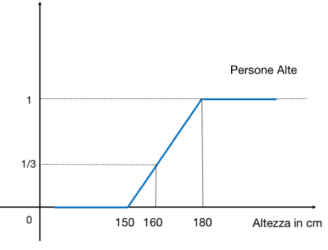
\includegraphics[width=0.5\textwidth]{img/sistemi_incerti/fuzzy.png}
    \caption{Esempio di rappresentazione grafica di un fuzzy set}
    \label{fig:fuzzy_set}
\end{figure}    
\begin{esempio}
    Insieme delle persone alte fino a $150$ si considera bassa,
    da $150$ a $180$ si può considerare medio alto e da $180$ è alto.
    La funzione potrebbe essere definita come 
    $$t(x) = \begin{cases}
        0& x\le 150\\
        \frac{x-150}{30}& 150\le x\le 180\\
        1& x\ge 180\\
    \end{cases}$$
\end{esempio}

I \textbf{fuzzy set}, a livello insiemistico, coincidono con l'insieme delle coppie 
elemento e grado di appartenenza. 

$$FS=\{(u, f(u)): u\in U, f(u)\in [0,1]\}$$

I \textbf{fuzzy set} possono essere \textbf{continui} o \textbf{discreti} se 
$U$ è \textbf{continuo} o \textbf{discreto}. Per gli insiemi continui ci sono alcune forme standard:
\begin{itemize}
    \item \textbf{triangolari}: dato $a<m<b$ allora sarà definito Così
    $$tr(x) = \begin{cases}
        0& x\le a\\
        \frac{x-a}{m-a} & x\in [a,m]\\
        \frac{b-x}{b-m} & x\in [m,b]\\
        0&x>b
    \end{cases}$$
    Usati nei Fuzzy control.
    \item \textbf{trapezioidali}: dati $a<m<n<b$ allora ho che da $[m,n]$ il grado
    di appartenenza che nel caso $m=n$ mi riconduco al triangolare
    \item \textbf{gaussiana}: dove
    $$g(x) = e^{-(\frac{(x-m)^2}{\sigma^2})}$$
    dove $m$ è il valore tipico 
\end{itemize}

\begin{definizione}
    Per un fuzzy set, l'insieme è \textbf{normale} se $\exists x, f(x) = 1$
\end{definizione}
\begin{definizione}
    Per un fuzzy set, il \textbf{support} è l'insieme tale che $\{x: f(x) >0\}$
\end{definizione}
\begin{definizione}
    Per un fuzzy set, il \textbf{core} è l'insieme tale che $\{x: f(x) =1\}$
\end{definizione}
\begin{definizione}
    Per un fuzzy set, $\alpha$-cut è l'insieme tale che $\alpha \in [0,1], \{x: f(x) \ge\alpha\}$
\end{definizione}
\begin{esempio}
    Dato un  $\alpha$-cut con $\alpha =1$ allora coincide con il sore set, mentre 
    quando $\alpha =0$ allora ottengo il support.
\end{esempio}

\begin{definizione}
    \textbf{strong} $\alpha$-cut è l'insieme tale che $\alpha \in [0,1], \{x: f(x) >\alpha\}$
\end{definizione}

I Fs sono degli insiemi e quindi possiamo definire le operazioni su insiemi $\cap, \cup, ^c, \subseteq$ 
partendo dagli insiemi normali quindi sulle funzioni caratteristiche, per poi 
mapparle sulle funzioni dei fuzzy:
\begin{itemize}
    \item \textbf{intersezione}: l'intesezione insiemistica classica 
    coincide con $(f\cap g)(x) = \min\{f(x), g(x)\}$ questo viene generalizzato dalle funzioni
    caratteristiche
    $$\mathcal{X}_A\cap \mathcal{X}_b = \begin{cases}
        1& \mathcal{X}_A(x) = 1\land \mathcal{X}_B(x)=1\\
        0& altrimenti
    \end{cases} \equiv 
    \min\{\mathcal{X}_A(x), \mathcal{X}_B(x)\}$$
    Quando siamo nel caso dei fuzzy set, $f(x), g(x) \in [0,1]$, allora $(f\cap g)(x)\in [0,1]$
    quindi coincide con la $t$-norma $(f\cap g)(x)= f(x) \ast g(x)$
    \item \textbf{unione}: l'unione insiemistica classica 
    coincide con $(f\cup g)(x) = \max\{f(x), g(x)\}$ questo viene generalizzato dalle funzioni
    caratteristiche
    $$\mathcal{X}_A\cup \mathcal{X}_b = \begin{cases}
        1& \mathcal{X}_A(x) = 1\lor \mathcal{X}_B(x)=1\\
        0& altrimenti
    \end{cases} \equiv 
    \max\{\mathcal{X}_A(x), \mathcal{X}_B(x)\}$$
    Quando siamo nel caso in cui $f(x), g(x) \in [0,1]$ allora $(f\cup g)(x)\in [0,1]$
    quindi coincide con la $t$-conorma $(f\cup g)(x)= f(x) + g(x)$ (coincide con $\max$)
    \item \textbf{complemento}: Quando siamo nel caso in cui $f(x), g(x) \in [0,1]$ allora $(f\cup g)(x)\in [0,1]$
    allora il complemento coincide con $1-f(x)$.
    \item \textbf{sottoinsieme}: nel caso delle funzioni caratteristiche 
     $\mathcal{X}_A\subseteq \mathcal{X}_B$
    è quando $\forall \mathcal{X}_A(x) \le \mathcal{X}_B(x)$ allora $f\subseteq g \iff \forall x, f(x)\le g(x)$.
    Questo può essere visto come l'operazione di $\implies$ infatti
    $$a\le b \iff a\implies b = 1$$

\end{itemize}

Abbiamo definito le operazioni in base alle $t$-norme e $t$-conorme, questo significa 
che possiamo definirle usano una delle varianti definite per la logica a valori 
infiniti.

\begin{esempio}
    Le varianti delle operazioni sono:
    \begin{itemize}
        \item $\min/\max$ (generalmente usata nei fuzzy)
        \item \textbf{Lukasiewicz} (l'intersezione nei fuzzy tende a schiacciare verso 0)
        \item \textbf{prodotto/somma probabilistica}
    \end{itemize}
\end{esempio}

Possiamo avere funzioni di aggregazione:
\begin{itemize}
    \item similarità: abbiamo il quasi associato alla proprietà
    \item incertezza: abbiamo il quasi associato al certamente. Teoria della possibilità 
    distribuzioni di possibilità
    \item preferenza:
\end{itemize}


\begin{definizione}[\textbf{Variabile linguistica}]
    In sostanza è una tupla $\langle L, T(L), G, U , M\rangle$ dove:
    \begin{itemize}
        \item $L$ è il nome della Variabile
        \item $T(L)$ insiemi di termini linguistici di $L$ ($L\in T(L)$) composto da 
        termini base e modificatori
        \item $G$ sono le regole con cui vando a mettere insieme i termini di base con i modificatori
        \item $U$ insieme universo, è il range dei valori che può assumere la variabile
        \item $M(x): U \to [0,1], \forall x\in T(L)$ assegna ad ogni termine un fuzzy set (dato un termine associanano un insieme fuzzy)
    \end{itemize} 
\end{definizione}

\begin{esempio}
    Un esempio può essere:
    \begin{itemize}
        \item $L=age$
        \item $G=linguistic_modifier+\{old, young\}$
        \item $T(L)=\{old,young, very_old,very_young, \dots\}$
        \item $U=[1,100]$
        \item $M(x):U\to [0,1], \forall x\in T(L)$, per esempio
        $$M(old)(u)=\begin{cases}
            \left[1+(\frac{u-50}{5})^{-2}\right]^{-1} & u\in [50,100]\\
            0 & u\in [0, 50)
        \end{cases}$$
        In questo caso si definisce $old$ da quando supera i $50$.
    \end{itemize}
\end{esempio}

Per assegnare una semantica numerica ai modificatori del linguaggio come tanto, molto,
poco, utilizziamo delle funzioni \textbf{modifier} che modifica l'incertezza di appartenenza degli 
elementi. La funzione sarà del tipo

$$m_A: [0,1]_A \to [0,1]_A$$

Le funzioni \textbf{modifier} si dividono in:
\begin{itemize}
    \item \textbf{concentration}: $con(f)(x)=[f(x)]^\beta, \beta>1$ da un significato di molto 
    quando il valore $\beta =2$. (concentro il fuzzy)
    \item \textbf{dilation}:  $dil(f)(x)=[f(x)]^\alpha, \alpha <1$ da un significato di abbastanza
    quando il valore $\alpha =\frac{1}{2}$. (allargo il fuzzy)
    \item \textbf{contrast intensifier}: modifica la confidenza degli elementi in modo 
    che si avvicini a $0$ o $1$ se rispettivamente $f(x)< 0.5$ e $f(x) >0.5$.
\end{itemize}

\begin{esempio}
    $vecchio(70)=0.94$ allora $molto_vecchio (70) = vecchio(70)^2$
    mentre $abbastanza_vecchio (70) = \sqrt{vecchio(70)}$
\end{esempio}

\begin{esempio}
    Per esempio un \textbf{contrast intensifier} definisce il modificatore $surely$
    attraverso le seguenti formule:
    $$sur(f)(x)=\begin{cases}
        2f^2(x) & f(x) \le 0.5\\
        1-2[1-f(x)]^2 & f(x) > 0.5
    \end{cases}$$
\end{esempio}

Ecco un immagine che mostra come si modifica la confidenza di un fuzzy utilizzando 
i modificatori (vedi \ref{fig:modificatori_fuzzy_set}).

\begin{figure}[!h]
    \centering
    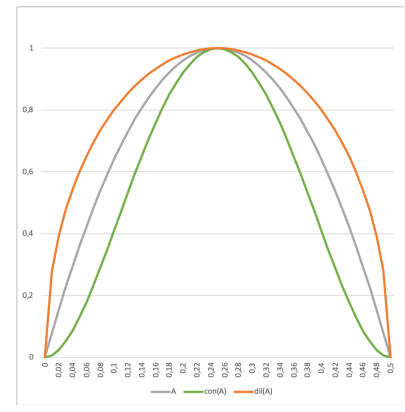
\includegraphics[width=0.5\textwidth]{img/sistemi_incerti/modificatori_fuzzy.png}
    \caption{Esempio di rappresentazione grafica di modificatori applicati ad un fuzzy set}
    \label{fig:modificatori_fuzzy_set}
\end{figure}  

Le variabili linguistiche permettono associare dei fuzzy set a dei concetti e 
mediante dei modificatori linguistici associare dei modificatori fuzzy per modificare 
la confidenza.

\subsection{Sistemi basati su regole}
I rules-based system sono sistemi specifici per dominio che usano delle regole 
per effettuare delle deduzioni o scelte.

I componenti base di questi sistemi sono (\ref{fig:rule-based}):
\begin{itemize}
    \item \textbf{base di conoscienza}: lista di regole di base che esprimono la 
    conoscenza del sistema nel dominio. L'espressione della base di conoscienza 
    si può fare attraverso due metodi:
    \begin{itemize}
        \item \textbf{mamdani}: regole if then con solo clausole formate da congiunzioni
        di espressioni boobleane in cui si testa il valore di alcune variabili linguistiche.
        \begin{center}
            IF ($X_1$ is $LT_1$) and \dots and ($X_n$ is $LT_n$) Then $Y$ is $LT_0$
        \end{center}
        Dove $X_i, Y$ sono variabili linguistiche e $LT_i$ sono i temini linguistici.
        \item  \textbf{sugeno}: cambiano le regole e permette di saltare il passo 
        di fuzzificazione.
        \begin{center}
            IF ($X_1$ is $LT_1$) and \dots and ($X_n$ is $LT_n$) Then $Y =p_0 + p_1X_1+ p_2X_2+\dots+ p_nX_n$
        \end{center}
        con $p=(p_0,\dots,p_n)$ vettore di numeri reali.
    \end{itemize}
    Essendo variabili linguistiche significa lavorare sui fuzzy.
    \item \textbf{inference engine}: effettua inferenza o prende decisioni in base alle interazioni 
    tra input e la base di conoscienza. Il processo di applicazione delle regole 
    si basa sui seguenti passi:
    \begin{itemize}
        \item \textbf{match}: si prende l'input si metcha con le regole, si possono 
        avere match multipli e ogni regola genera un risultato. Alla fine si avrà 
        un insieme di risultati chiamato \textbf{conflict set}.
        \item \textbf{conflict-resolution}: si agrega ciascun risultato del 
        \textbf{conflict set} in modo da ottenure un unico valore.
        \item \textbf{esegue}: ottenuto il valore attuale effettua l'azione 
        desiderata
    \end{itemize}
\end{itemize}

\begin{figure}
    \centering
    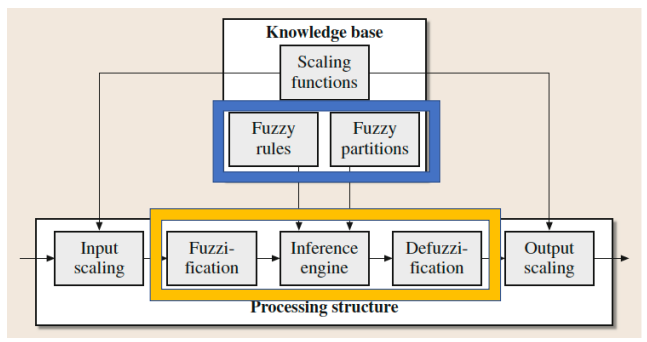
\includegraphics[width=0.5\textwidth]{img/sistemi_incerti/rule-based-system.png}
    \caption{Schema dei rule-based system}
    \label{fig:rule-based}
\end{figure}

Quindi dal mondo reale otteniamo un insieme di valori reali che descrivono 
la situazione, questi devono poi essere mappati sugli insiemi fuzzy associati (fuzzyficazione),
successivamente avendo i fuzzy si applica una regola alla volta, in modo da produrre 
un valore del fuzzy di output per ogni regola. Per produrre un valore di output 
per ogni regola, si applicano le $t$-norme e le $t$-conorme sui fuzzy delle regole 
in base ai connettivi. Quindi se abbiamo $m$ regole, otteniamo $m$ valori del 
fuzzy di output, quindi dovremo aggregarle, per fare ciò si usa la $t$-conorma ($\max$).

In questo modo otteniamo un unico valore di fuzzy in output, infine dobbiamo riconvertire
 il valore in numero reale e questo può essere vatto in due metodi:
\begin{itemize}
    \item \textbf{mean of maxima}: si estrae il valore 
    $$x^\ast = (a+b)/2$$
    dove $a = \inf\{x|B(x) = \max_y B(y)\}$ e  $b = \sup\{x|B(x) = \max_y B(y)\}$,
    ovvero coincide al valore medio dell'intervallo di valori di massima confidenza 
    del fuzzy di output ($B(x)$).
    \item \textbf{center of gravity}: si effettua una media pesata dei valori 
    del fuzzy per la loro confidenza
    $$x^\ast = \frac{\int_x x\cdot B(x)dx}{\int_x \cdot B(x)dx} \equiv x^\ast =\frac{\sum_x x\cdot B(x)dx}{\sum_x \cdot B(x)dx} $$
\end{itemize}

La parte di fuzzyficazione può essere fatta di due modi:
\begin{itemize}
    \item \textbf{FATI}: come spiegato prima, sia $B_i(y)$ il valore del fuzzy di 
    output dell'$i$-esima regola allora si calcola $B(y)= G(B_1(y),\dots, B_m(y))$
    ($G\equiv \max$) e poi inferisco il valore finale $Y_0=D(B(y))$ ($D\equiv$ center of 
    gravity o mean of maxima).
    \item \textbf{FITA}: per ogni regola ottengo $B_i(y)$ il valore del fuzzy di 
    output dell'$i$-esima regola allora effettuo subito l'inferenza per ogni 
    regola ottenendo il valore $y_i=D(B_i(y))$, infine aggrego i valori inferiti 
    pesandoli per la $t$-norma dei fuzzy di input $y=\frac{\sum y_i\cdot h_i}{\sum h_i}$
    dove $h_i=\ast(A_1(x_1),\dots,A_n(x_n))$.
\end{itemize}
\begin{nota}
Le regole possono essere attivate insieme e le posso rappresentare come una tabella 
se le regole sono poche.
\end{nota}

Spesso in output alle regole posso avere un singleton fuzzy ovvero quando abbiamo 
un unico valore a $1$ e tutto il resto a $0$ per ogni regola.

\section{Rough set}

Sono delle varianti di insiemi che permettono di effettuare operazioni di feature 
selection, Rough clustering e trovano applicazione anche ai sistemi dinamici.
I Rough set a livello generale sono degli insiemi di cui conosciamo con certezza 
solo alcuni elementi che appartengono e alcuni elementi che non appartengono, ma 
abbiamo elementi che forse appartengono o forse no.

\begin{definizione} [\textbf{information table} (information system)]
    L'\textbf{information table} $S(U) = \langle U, Att, Val, F\rangle$ dove:
    \begin{itemize}
        \item $U$ è un insieme di Oggetti
        \item $Att$ è un insieme di attributi
        \item $Val$ è un insieme di valori degli attributi
        \item $F:U\times A \to Val$ è una funzione che ad ogni oggetto ritorna il 
        valore dell'attributo scelto
        \item 
    \end{itemize}
\end{definizione}
\begin{esempio}
    Datta la seguente tabella informativa.
    \begin{figure}[!h]
        \centering
        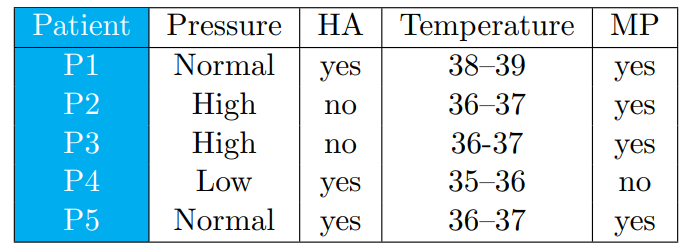
\includegraphics[width=0.5\textwidth]{img/sistemi_incerti/i_t.png}
    \end{figure}
    possiamo identificare:
    \begin{itemize}
        \item l'insieme degli oggetti $\{P_1,\dots,P_5\}$
        \item l'insieme degli attributi $\{Pressure, HA, Temperature,MP\}$
        \item l'insieme dei valori $\{Yes, No, 37-38,\dots\}$
        \item $F(P2, Pressure)=High$
    \end{itemize}
\end{esempio}
\begin{definizione}[\textbf{Decision system}]
    Un \textbf{decision system} $S(U) = \langle U, C\cup \{d\}, Val, F\rangle$ dove:
    \begin{itemize}
        \item $U$ è un insieme di Oggetti
        \item $C$ è un insieme di attributi dette condizioni
        \item $\{d\}$ è l'insieme di attributi di decisione
        \item $Val$ è un insieme di valori degli attributi
        \item $F:U\times C\cup \{d\} \to Val$ è una funzione che ad ogni oggetto ritorna il 
        valore dell'attributo scelto
        \item 
    \end{itemize}
\end{definizione}
In sostanza si aggiunge l'attributo decisione che corrisponde alla classe degli oggetti.
Possiamo raggruppare gli oggetti rispetto all'attributo decisione, questo mi permette 
di definire delle \textbf{classi di decisione} (insiemi $U_d = \{u\in U: F(u, decision) =d\}$) 

Il sistema viene definito:
\begin{itemize}
    \item \textbf{consistente}: se ogni coppia di oggetti che hanno attributi uguali 
    afferiscono alla stessa classe di decisione
    \item \textbf{inconsistente}: se esiste una  coppia di oggetti
    con attributi uguali e classi di decisione diverse
\end{itemize}

\begin{definizione} [\textbf{Relazione di Indiscernibilità}]
    Dato un sottoinsieme di attributi $A\subseteq Att$, due oggetti $x,y\in U$ sono 
    \textbf{indiscernibilità} rispetto a $A$ se 
    $$\forall a \in A, F(a, x) = F(a,y)$$
    Si scriverà $xI_A y$.
\end{definizione}
$I_A$ è una relazione di equivalenza perché è riflessiva, simmetrica e transitiva.
Questo significa che partiziona $U$ in classi di equivalenza chiamate anche \textbf{granularità 
delle informazioni}.
$$[x]_A:=\{y\in U:xI_Ay\}$$

\begin{definizione}[\textbf{Decisione generalizzata}]
    Una decisione generalizzata è una funzione decisione $\delta_A: U \to \mathcal{P}(Val)$
    tale che 
    $$\delta_A(x) = \{i \in Val: \exists y, xI_A y \land F(y,d) = i \}$$
\end{definizione}

La funzione di decisione generalizzata ritorna l'insieme delle decisioni di tutti 
gli oggetti che condividono gli stessi attrbuti dell'oggetto di input.

\begin{nota}
    Un sistema è \textbf{consistente} sse $|\delta_A(x)| = 1,\forall x\in U$.
\end{nota}

Data una partazione degli oggetti mediante l'indiscernibilità $\{P_1\}, \{P_2,P_3\}, 
\{P_4\}, \{P_5\}$, possiamo identificare un insieme normale $H = \{P_1\}\cup\{P_2,P_3\}$, 
che è certo, mentre possiamo definire $K=\{P_1,P_2\}$  che è un insieme \textbf{rough}
perché $P_2$ non conosciamo in che partizione si trova e infatti $K$ può essere approssimato 
tra due insiemi esatti (ovvero partizioni).
$$\{P_1\} \subseteq K \subseteq \{P_1,P_2,P_3\}$$


\begin{definizione}[\textbf{Approssimizzazioni}]
    Sia $S(U) = \langle U, Att, Val, F\rangle$ un information table. Dato un insieme 
    di attributi $A\subseteq Att$, allora per ogni $H\subseteq U$ definiamo:
    \begin{itemize}
        \item \textbf{lower approximation} di $H$:
        $$L(H):= \{x: [x]_A\subseteq H\}$$
        \item \textbf{upper approximation} di $H$:
        $$U(H):= \{x: [x]_A \cap H\ne \emptyset\}$$
    \end{itemize}
\end{definizione}

\begin{definizione}[\textbf{Rough}]
    La coppia $r(H) = \langle L(H), U(H)\rangle$ è chiamato \textbf{rough approximation} o
    \textbf{rough set}.
\end{definizione}
Ecco un esempio di rough set \ref*{fig:rs}.

\begin{figure}[!h]
    \centering
    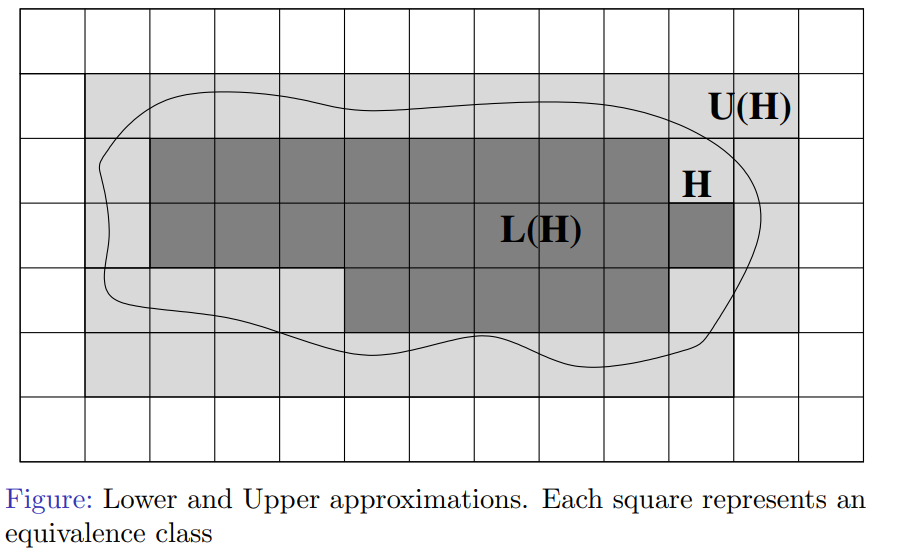
\includegraphics[width=0.5\textwidth]{img/sistemi_incerti/rs.png}
    \caption*{Esempio di Rough set}
    \label{fig:rs}
\end{figure}

Definiremo:
\begin{itemize}
    \item \textbf{esterior}: $E(H) = U^c(H), L(H)\cap E(H) = \emptyset$ ovvero gli 
    le classi che sicuramente non appartengono al rough
    \item \textbf{Boundary}: $Bnd(H) = U(H) - L(H)$ ovvero 
    le classi su cui abbiamo incertezza sull'appartenenza.
\end{itemize}

Possiamo misurare la grandezza del boyndary utilizzando le misure di incertezza:
\begin{itemize}
    \item \textbf{accuracy}: $\alpha(H) = \frac{|L(H)|}{|U(H)|}$
    \item \textbf{roughness}: $1-\alpha(H) = \frac{|Bnd(H)|}{|U(H)|}$
\end{itemize}

Le approssimazioni dall'alto e dal basso rispettano le seguenti proprietà:
\begin{itemize}
    \item $L(\emptyset)= \emptyset$, $L(U)=U$ uguale per l'approx alto
    \item $L(H)\subseteq H$ $H\subseteq U(H)$ 
    \item distributività $L(H\cap K)= L(H) \cap L(K) $, $L(H) \cup L(K) \subseteq L(H\cup K) $ contrario per l'approx alto
    \item monotonia $H\subseteq K\implies L(H)\subseteq L(K)$ uguale
    \item idempotenti $L(L(H)) = L(H)$ e $L(U(H)) = U(H)$
    \item dualità $L(H) = (U(H^c))^c$
\end{itemize}

\begin{nota}
    Queste sono proprietà tipiche di uno spazio topologico e sono operatori dipici
    delle logiche modali.        
\end{nota}

Fino ad ora abbiamo definito tutte i rough set tramite relazioni di equivalenza,
ma questo è troppo restrittivo, quindi possiamo generalizzare il ragionamento a una 
relazione $R$ "qualsiasi" (se $R$ è una relazione di equivalenza allora torno a prima). 
In realtà non possiamo estendere ad una $R$ binaria generica perché perdiamo 
alcune delle prorpietà introdotte prima. 
Definiamo una generica relazione $R\subseteq U\times U$, definiamo la granularità
dell'informazione $g_R(x) = \{y\in U: xR y\}$ allora otteniamo le seguenti approssimazioni
$$l_R(H) = \{x\in U:g_R(x)\subseteq U\}$$
$$u_R(H) = \{x\in U:g_R(x)\cap U = \emptyset\}$$

Si mantengono quindi le seguenti prorpietà per ogni $R$ scelta:
\begin{itemize}
    \item $l_R(U) = U$ 
    \item $u_R(\emptyset) = \emptyset$
    \item $l_R,u_R$ sono monotone
\end{itemize} 
Dobbiamo solo chiedere che $R$ rispetti:
\begin{itemize}
    \item \textbf{serialità} (no punti isolati): che ci aggiunge le proprietà $l_R(H) \subseteq u_R(H)$,
    $u_R(U) =U$ e $l_R(\emptyset) = \emptyset$.
    \item \textbf{riflessività}: che ci aggiunge le proprietà $l_R(H)\subseteq H \subseteq u_R(H)$
\end{itemize}

\begin{nota}
    se una relazione è \textbf{riflessiva} allora è anche \textbf{seriale}
\end{nota}

Se condidero rough set con $\mathcal{R}$ di similarità, sono certo che questa è simmetrica 
e riflessiva quindi perdiamo solo la transitività dalle relazioni di equivalenza.

Possiamo considerare i seguenti esempi:
\begin{itemize}
    \item $\mathcal{R}$ associata alla distanza tra oggetti utilizzabile quando 
    abbiamo piena conoscienza degli attributi degli oggetti
    \item $\mathcal{R}$ gestire valori mancanti
    $$x\mathcal{R}_Dy\iff \forall a_i\in D, F(x, a_i) = F(y,a_i) \lor F(x, a_i)=\ast \lor F(y, a_i)=\ast $$
    \item $\mathcal{R}$ gestire valori incompleti o parziali
    $$x\mathcal{R}_Dy\iff \forall a_i\in D, F(x, a_i) \cap F(y,a_i) \ne \emptyset$$
\end{itemize}

\subsection{Reduct}

I Rough set permettono di calcolare i reduct, ovvero gli insiemi di attributi più 
significativi per prendere una decisione e questi sono utili per definire delle 
regole per effettuare le decisioni a partire dal sottoinsieme di attributi.

Scelta la tabella, per calcolare i reduct posso calcolare la partizione degli oggetti 
eliminando ogni volta uno o più attributi, l'insieme di attributi minimo che preserva 
la partizione iniziale coincide con un \textbf{Reduct}. 

\begin{definizione}[\textbf{Reduct}]
    Sia $A\subseteq B\subseteq Att$, $A$ è un \textbf{reduct} di $B$ se :
    \begin{itemize}
        \item $\Pi_A = \Pi_B$
        \item $\not\exists C \subset A, \Pi_C=\Pi_B$
    \end{itemize}
    insieme minimale di attributi che mi rappresenta la stessa partizione (preservazione 
    della partizione e minimalità)
\end{definizione}
\begin{definizione}[\textbf{attributo indispensabile}]
    Sia $a \in A\subseteq Att$ è un \textbf{attributo indispensabile} in $A$ se $\Pi_A \ne \Pi_{A-\{a\}}$
\end{definizione}
\begin{definizione}[\textbf{Core}]
    Il \textbf{Core} è l'insieme indispensabile di attributi in $Att$ ovvero l'intersezione 
    di tutti i reduct in $Att$.
\end{definizione}

Dati $n$ attributi allora esistono $\mathcal{O} \left(\frac{3^n}{\sqrt{n}}\right)$ reduct.

Trovare il reduct più piccolo è più di NP completo e quindi una soluzione è parallelizzare 
oppure si devono utilizzare delle euristiche.


\subsection{Sistemi basati su regole}
Posso utilizzare i Rough set per i sistemi basati su regole. 

Se siamo nel caso di sistemi consistenti, dato un reduct allora si possono definire
delle regole in base ai valori che assumono gli attributi, in questo modo possiamo 
effettuare delle decisioni.

\begin{figure}[!h]
    \centering
    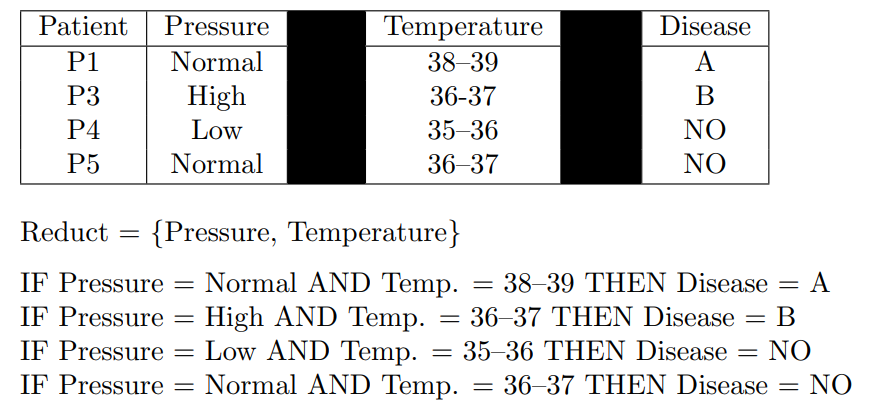
\includegraphics[width=0.5\textwidth]{img/sistemi_incerti/rule-based-system-rough.png}
\end{figure}

In caso di sistemi inconsistenti, il ragionamento cambia e non possiamo più basarci 
sulla \textbf{decisione} esata degli oggetti, bensì dobbiamo basarci sulla 
\textbf{decisione generalizzata}.

\begin{definizione}[\textbf{Estensione reduct alla decisione generalizzata}]
    Sia $A\subseteq B\subseteq Att$, $A$ è un \textbf{reduct} di $B$ se:
    \begin{itemize}
        \item $\delta_A = \delta_B$ (rimuovo inconsistenza)
        \item $\not\exists C \subset A, \delta_C=\delta_B$
    \end{itemize}
\end{definizione}

In questo modo risolvo l'inconsistenza a discapito di un'incertezza nelle regole,
infatti non ho una classificazione corretta, ma è sempre una classificazione ambigua ma senza errori.

\begin{figure}[!h]
    \centering
    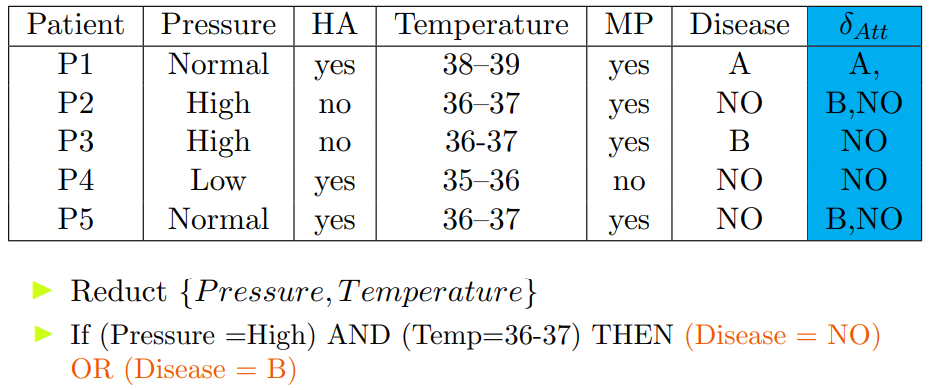
\includegraphics[width=0.5\textwidth]{img/sistemi_incerti/rule-based-system-rough-apr.png}
\end{figure}

Un altra soluzione all'inconsistenza del sistema  è valutare l'\textbf{indipendenza degli attributi}, 

\begin{definizione}[\textbf{Coefficiente di dipendenza}]
    sia $S(U)$ un decision system, sia $A\subseteq Att$ un insieme di attributi,
    $X_i$ le classi di decisione. Il \textbf{coefficiente di dipendenza} di decisione 
    $d$ dagli attributi $A$ è 
    $$Dip(A, d) = \frac{\sum |L_A(X_i)|}{|X|}$$

\end{definizione}

Il coefficiente specifica quanti oggetti riesco a caratterizzare con certezza per 
l'insieme di attributi $A$ sulla decisione $d$ ($Dip(A, d) =1$ è un sistema consistente). 

\begin{definizione}[\textbf{Estensione reduct al coefficiente di dipendenza}]
    sia $S(U)$ un decision system,  $A\subseteq B\subseteq Att$, $A$ è un \textbf{reduct} di $B$ se:
    \begin{itemize}
        \item $Dip(A,d) =Dip(B,d)$ (rimuovo inconsistenza)
        \item $\not\exists C \subset A, Dip(C,d) =Dip(B,d)$
    \end{itemize}
\end{definizione}

\begin{figure}[!h]
    \centering
    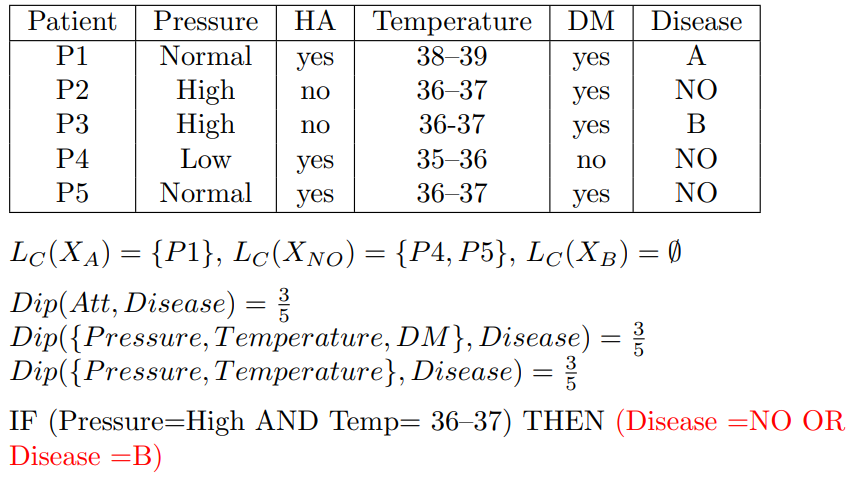
\includegraphics[width=0.5\textwidth]{img/sistemi_incerti/rule-based-system-rough-apr2.png}
\end{figure}

Un modo per alleggerire le varie richieste è quello di considerare reduct approssimati,
quindi non vado più a valutare attributi indispensabili/inutili, valuto quanto 
un attributo è significativo. 

Utilizziamo il coefficiente di dipendenza e valuto quanto 
varia il ocefficiente eliminando una porzione degli attributi.
$$Dip(C,d) = \frac{\sum_{min}^{max}|L_C(U_i)|}{|U|}$$
quindi ogni volta probo a rimuovere $B$ attributi e calcolo quanto varia il coefficiente
di dipendenza, se rimane sotto una soglia allora va bene altrimenti cerco nuovi 
attributi.
$$\frac{Dip(C,d)-Dip(C-B,d)}{Dip(C,d)} = \begin{cases}
    =0 & \text{def prec.}\\
    \le \epsilon 
\end{cases}$$

\begin{nota}
    In caso di attributi continui si fa una discretizzazione.
\end{nota}

Le regole le definiamo in questo modo 
$$r:U \to (d=v)$$
$match(r) = |U|$
$support(r) = |U\cap (d=v)|$
$consistenza = \frac{support(r)}{match(r)}$
$u$ oggetti.$(d= v)$ decisione uguale $v$

$r=(temp = 36-37)\to (D=no)$ in numero di oggetti che metchnano è $match(r)=3$ 
mentre $support(r)= 2$ quanti sono $no$ tra quelli che metchano.


\begin{esempio}
    Data la relazione $xI_Ay$ di discernibilità, abbiamo $n$ oggetti $|U|=n$ allora 
    dobbiamo definire una matrice $n\times n$ 
    $$c_{ij}= \{a\in A: F(a,x_i)\ne F(a,x_j)\}$$
    $A$ attributi.
$$
    \begin{array}{cccccc}
        x_U & a&b&c&d&e\\
        x_1 & 0&1&1&1&1\\
        x_2 & 1&1&0&1&0\\
        x_3 & 1&0&0&1&1\\
        x_4 & 1&0&0&1&0\\
        x_5 & 1&0&0&0&0\\
        x_6 &1&1&0&1&1\\
    \end{array}
    $$  
    La matrice di discernibilità è simmetrica e sulla diagonale $\emptyset$ e 
    $d_{ij}$ contiene di tutti gli attributi comuni a $x_i,x_j$.   
    $$
    \begin{array}{ccccccc}
        x_U & x_1 & x_2 & x_3 & x_4 & x_5 & x_6 \\
        x_1 & &1&1&1&1\\
        x_2 & \{a,d,e\}&1&0&1&0\\
        x_3 & \{a,c,d,e\}&0&0&1&1\\
        x_4 & 1&0&0&1&0\\
        x_5 & 1&0&0&0&0\\
        x_6 &1&1&0&1&1\\
    \end{array}
    $$

    Questa mi permette di ottenere il $core=\{a\in A: c_{ij}= \{a\}\}$

    Per calcolare i reduct: definsco una funzione booleana basandomi sula matrice 
    discernibilità composta da conciuzioni degli elementi $\lor c_{ij}$ 
    $$f(a,b,c,d,e,o)=(a\lor d\lor o)\land (a\lor d\lor c\lor e)$$

    and di tutte le entry della matrice di discernibilità, ogni entri coincide con un 
    or degli attributi. elimino le clasole contenenti elementi minimali

    $$f(a,b,c,d,e,o)= c\land e\land o \land (a\lor d)\land \dots$$
    La devo trasformare in forma normale disgiunta
    $$f(a,b,c,d,e,o)= (c\land e\land o \land a)\lor(c\land e\land o \land d)$$
    e questi sono tutti i reduct $c\land e\land o \land a$ e $c\land e\land o \land d$.
    Quello che abbiamo fatto è calcolcare gli implicanti primi della funzione booleana
    ovvero mi basta conoscere questi valori per decidere la tabella finale.
\end{esempio}

Abbiamo La matrice di discernibilità permette di avere un modo per calcolare i reduct 
attraverso la riduzione.
\subsection{Fuzzy Rough Set}
noi abbiamo fuzzy per rappresentare il vago e poi abbiamo Roughset che mi permette 
di suddividere gli oggetti, ovvero la granularità dell'universo (basati su insiemi e relazioni)
Possiamo unire i concetti usando fuzzy set e relazione fuzzy (quanto un elemento è
in relazione con un elemento). Per definire le approssimazioni si usano le $t$-norme 
e $t$-conorme (approssimo un insieme fuzzy attraverso due insiemi fuzzy).


\section{Orthopairs}
Sono la generalizzazione dei Roughset 
\begin{definizione}[\textbf{Orthopair}]
    L'\textbf{orthopair} è una coppia $(A,B)$ ortogonale o disgiunta di sottoinsiemi
    dell'insieme universo $X$: $A,B\subseteq X$ e $A\cap B=\emptyset$
\end{definizione}
\begin{definizione}[\textbf{Nested pairs}]
    L'\textbf{nested pairs} è una coppia $(A,C)$ equivalente all'ortopair tale che 
    $A\subseteq C \subseteq X$ e $C =B^c$
\end{definizione}

L'interpretazione associata all'orthopair $(P,N)$ è $P$ elementi positivi e $N$ 
elementi negativi.

Identifichiamo per l'orthopair il \textbf{boundary} $Bnd=(P\cup N )^c$ e quindi 
definiamo con un orthopair una \textbf{tripartition} dell'universo.

\begin{nota}
    $(P,Bnd)$ e $(N, Bnd)$ sono a loro volta delle orthopair perché sono insiemi disgiunti.
\end{nota}

\begin{esempio}
    Pari e dispari
    caso booleano insieme di variabili vere e false, in bnd è l'incertezza.
\end{esempio}

\begin{definizione}[\textbf{Consistenza}]
    Un insieme $S$ è \textbf{Consistente} con un'orthopair $O = (P,N)$ se 
    $$s\in P \implies x\in S\land x\in N \implies x\not \in S$$
\end{definizione}

\begin{esempio}
    Data l'ortocoppia $O=(\{1,3\}, \{2,4\})$ allora $S_1=\{1,3\}$ e $S_2=\{1,3,5\}$ 
    sono consistenti con $O$, al contrario $S_3=\{1,2,3,5\}$ e $S_4=\{1,5\}$ non sono 
    consistenti con $O$.
\end{esempio}

\begin{definizione}[\textbf{Disjoint}]
    Due orthopairs $O_1,O_2$ sono \textbf{disjoint} se:
    \begin{itemize}
        \item $P_1\cap P_2=\emptyset$
        \item $P_1\cap Bnd_2=\emptyset\land  Bnd_1\cap P_2=\emptyset$
    \end{itemize}
\end{definizione}

Possiamo ottenere delle orthopair a partire dai Roughset che possiamo vederli come 
$(L(H),U^c(H))$ o $(L(H),Bnd(H))$. Altrimenti possiamo tenerli da \textbf{modelli 
partziali}, ovvero si assegna un valore di verità per ogni elemento dell'insieme 
universo tale che sia consistente con l'orthopair. Questi modelli rispecchiano 
il significato di consistenza.
\begin{esempio}
    Sia $(P = \{x_1,x_4\},N =\{x_3\})$ allora possiamo pensare di avere i seguenti 
    modelli parziali:
    \begin{itemize}
        \item $v_1:= x_1=x_4=x_2 = true, x_3=false$
        \item $v_2:= x_1=x_4= true, x_3=x_2 =false$
    \end{itemize}
    Entrambi i modelli soddisfano l'orthopair, in generale tutti i modelli che 
    soddisfano l'orthopair sono quegli assegnamenti degli elementi tali che tutti 
    gli elementi di un insieme devono avere lo stesso valore ma diverso dagli elementi 
    dell'altro insieme. L'assegnamento agli elementi del boundary può essere fatto 
    come si vuole (incertezza). 
\end{esempio}

Le orthopair possono essere ottenute dai \textbf{Shadow set} che sono approssimazioni 
dei Fuzzy set mediante i valori $\{0, [0,1], 1\}$.

Infine gli orthopair possono essere ottenuti dalle \textbf{informazioni bipolari}
del mondo.

Esistono delle generalizzazioni delle orthopairs chiamate \textbf{Fuzzy orthopair} o \textbf{insiemi
fuzzy intuizionistici}. L'orthopair è una coppia di fuzzy $f_P,f_N:X\to \{0,1\}$
tale che $\forall x\in X, f_P(x)+f_N(x) \le 1$.

Un'altra generalizzazione è la \textbf{teoria della possibilità}, ovvero si ha un insieme 
di valutazioni $E$ arbitrarie, la classe dell'orthopair coincide  con la particolare 
classe \textbf{hyper-rectangular boolean possibility distributions} sullo spazio 
$\{0,1\}^n $.

Alle orthopair possiamo ritornare alle logiche a 3 valori. A partire da un universo 
$X$, si definisce $f: X \to \{0,\frac{1}{2},1\}$ tale che 
$$f(x) = \begin{cases}
    1&x\in A\\
    0&x\in B\\
    \frac{1}{2}&altrimenti\\
\end{cases}$$
Quindi possiamo definire una orthopair $(A_1,A_0)$ tale che 
$$A_1:=\{x:f(x)=1\} \qquad \text{dominio certo}$$
$$A_0:=\{x:f(x)=0\}\qquad \text{dominio impossibile}$$

In questo modo possiamo mappare i connettivi delle logiche a $3$ valori sulle orthopair 
o nestedpair.

\begin{figure}[!h]
    \centering
    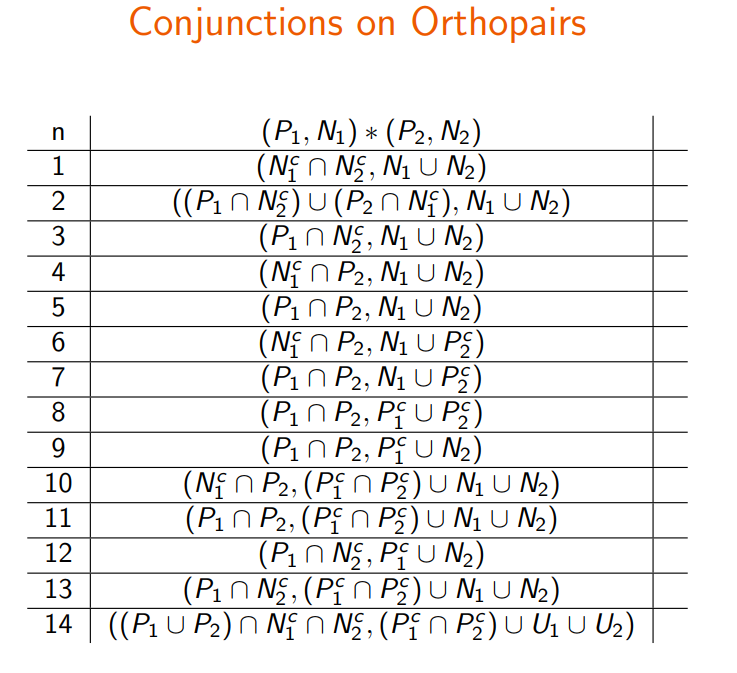
\includegraphics[width=0.5\textwidth]{img/sistemi_incerti/conj_ortho.png}
\end{figure}

\begin{figure}[!h]
    \centering
    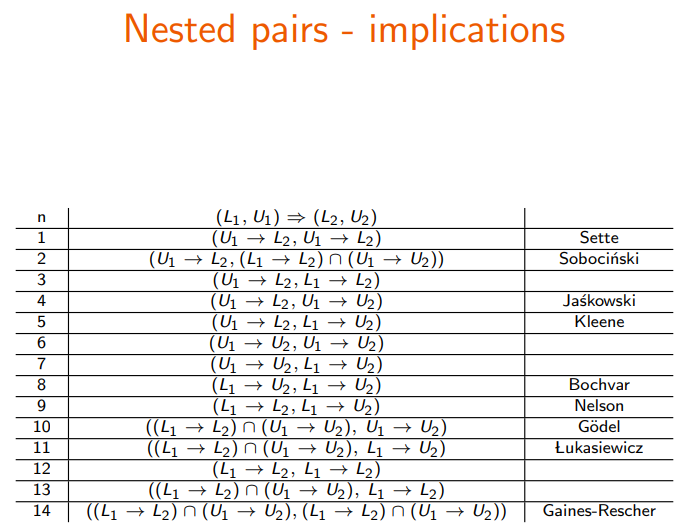
\includegraphics[width=0.5\textwidth]{img/sistemi_incerti/impl_nested_pair.png}
\end{figure}

Possiamo definire delle relazioni di ordinamento rispetto agli elementi dell'insieme 
universo in base ai valori di verità specificati dall'orthopair.

\begin{figure}[!h]
    \centering
    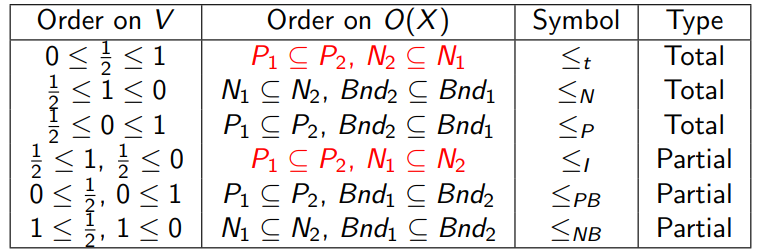
\includegraphics[width=0.5\textwidth]{img/sistemi_incerti/ordering.png}
\end{figure}

Possiamo identificare i seguenti ordinamenti importanti:
\begin{itemize}
    \item \textbf{ordine di verità} $O_1\le_t O_2$: $O_2$ è più vera rispetto $O_1$, ordine totale rispetto al valore di verità
    \item \textbf{ordine di conoscienza} $O_1\le_l O_2$: $O_2$ è più informativa rispetto $O_1$ (boundary più piccolo), ordine parziale rispetto all'incertezza
    in cui $0,1$ non sono confrontabili ma ci interessa solo il confronto tra l'incertezza
    e la certezza.
\end{itemize}

Definendo un ordinamento totale basato sui $3$ valori, possiamo derivare quindi delle operazioni 
di meet e join derivate dalle logiche a $3$ valori.

\begin{figure}[!h]
    \centering
    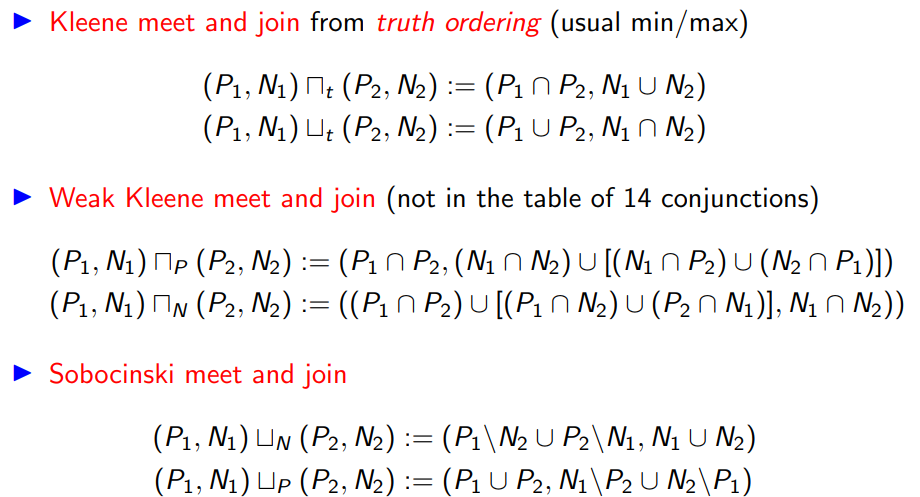
\includegraphics[width=0.5\textwidth]{img/sistemi_incerti/op_ortho.png}
\end{figure}


Definendo un ordinamento parziale basato sui $3$ valori, possiamo derivare quindi delle operazioni 
di meet e join derivate dalle logiche a $3$ valori, hanno senso solo quando si mantiene 
la consistenza delle orthocoppie, ovvero quando non si ocntraddicono.

\begin{figure}[!h]
    \centering
    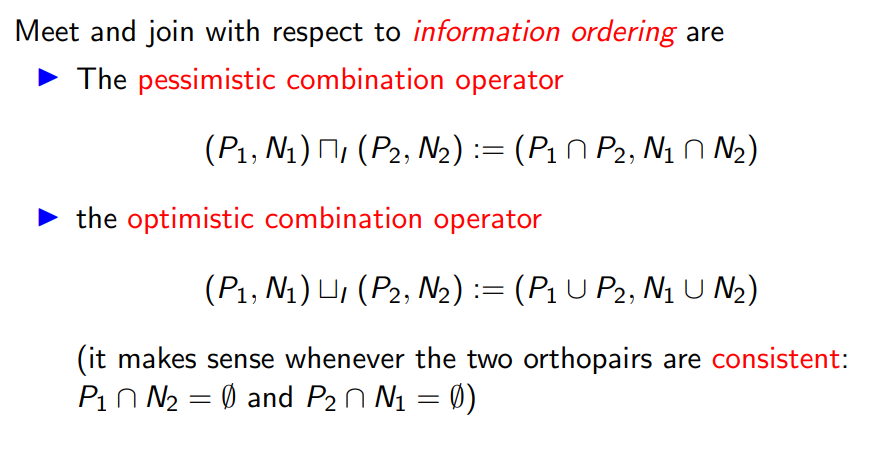
\includegraphics[width=0.5\textwidth]{img/sistemi_incerti/op_orthon_r.png}
\end{figure}

Si chiama operatore pessimistico perché prendo solo la conoscienza comune, mentre 
l'operatore ottimistico è un'operazione solo quando le ortocoppie sono consistenti e 
fa l'unione della conoscienza.

In aggiunta dal significato delle orthopair possiamo definire l'operatore di \textbf{consenso}
$$O_1 \odot O _2 = (O_1 \ominus O _2) \sqcup_l (O_2 \ominus O_1)$$
dove $O_1 \ominus O _2 :=  (P_1-P_2,N_1-N_2)$ è l'operatore di \textbf{differenza}.
L'operatore mi calcola ciò su cui sono d'accordo.
\begin{esempio}
    Sia $O_1=(\{x_1,x_2\},\{x_3,x_4\})$ con $x_1,x_2$ true e $x_3,x_4$ sono falsi.
    Sia $O_1=(\{x_1,x_3,x_4\},\{x_2,x_4,x_6\})$ con $x_1,x_3,x_4$ true e $x_2,x_4,x_6$ sono falsi.

    Allora $O_1 \odot O _2 = (\{x_1,x_5\},\{x_4,x_6\})$. 
\end{esempio}

Date due orthopair che rappresentano l'opinione di due agenti allora possiamo dire:
\begin{itemize}
    \item $\odot$: permette di ottenere l'accordo tra le due opinioni
    \item $\sqcap_l, \sqcup$: permettono di raggruppare le opinioni in modo pessimistico 
    o ottimistico
\end{itemize}

Nel caso di orthopair che rappresentano l'accettazione o il rigetto, le operazioni 
possono essere utilizzate per aggregare differenti decisioni. 

\begin{esempio}
    Queste operazioni permettono di unire risultati di classificazione.
    
\end{esempio}

I Roughset sono un sottoinsieme delle orthopair, infatti un generico $R(X)= (l(X), u(X))$ 
può essere associato ad un nestedpair e quindi un orthopair, perciò possiamo estendere 
tutte le operazioni sulle orthopair ai roughset.
Quindi possiamo combinare due Roughset usando le operazioni sulle orthopair che sono 
chiuse sui roughset. 

\begin{figure}[!h]
    \centering
    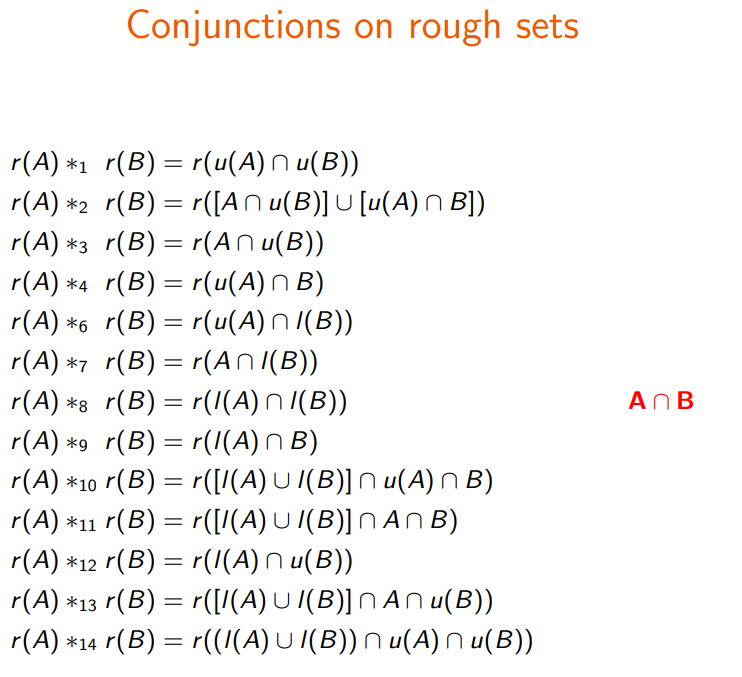
\includegraphics[width=0.5\textwidth]{img/sistemi_incerti/conj_RS.png}
\end{figure}

\begin{figure}[!h]
    \centering
    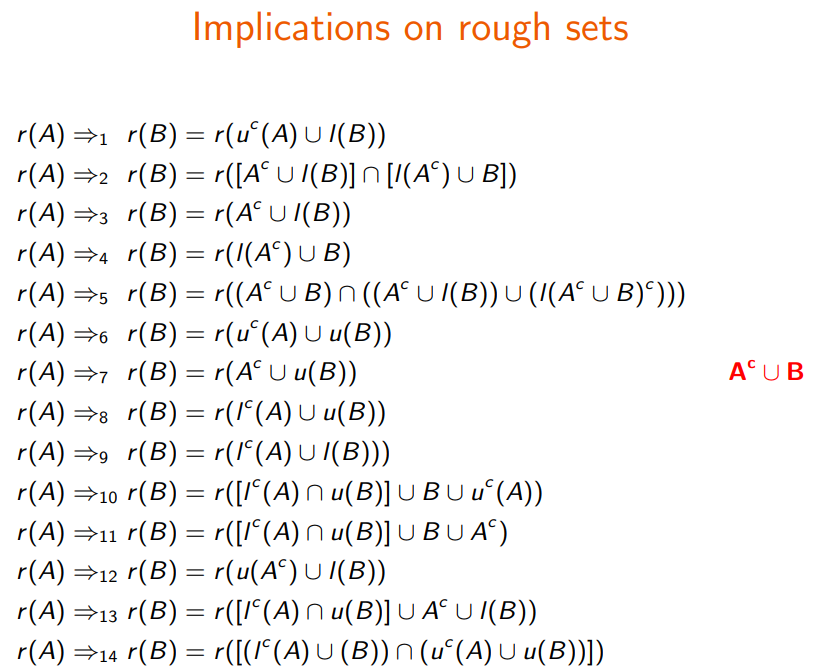
\includegraphics[width=0.5\textwidth]{img/sistemi_incerti/impl_RS.png}
\end{figure}

In generale dati due RS $r(A) = (l(A), u(A))$ e $r(B)=(l(B),u(B))$ allora si 
definisce l'unione e l'intersezione  come 
$$r(A)  \sqcap r(B) = (l(A)\cap l(B),u(A)\cap u(B))$$
$$r(A)  \sqcup r(B) = (l(A)\cup l(B),u(A)\cup u(B))$$

sappiamo che $r(A)  \sqcap r(B)$ e $r(A)  \sqcup r(B)$ sono proprio dei roughset,
supponiamo che siamo rispettivamente $r(C)$ e $r(D)$, in generale $C\ne A\cap B$ e $D\ne A\cup B$.

Per l'unione abbiamo diverse definizioni:
\begin{itemize}
    \item $C= [l(A)\cap l(B)] \cup Y$, $Y$ corrisponde ad un elemento scelto in una 
    classe di equivalenza, quindi si hanno diverse definizioni.
    \item $C=(A\cap B) \cup ((A\cap u(B))\cap(u(A\cap B)^c))$, in questo caso non 
    è simmetrica in $A,B$, quando $B=A^c$ allora $C\ne \emptyset$.
\end{itemize}

approssimazione C' è intersezione delle approssimazioni di A e B. La situazione è 
duale per $D$.

La scelta su come calcolare $C,D$ porta a dei problemi di interpretazione infatti 
abbiamo $2$ livelli di interpretazione:
\begin{itemize}
    \item linguaggio di insiemi (estensione): quando si lavora con le classi di equivalenza
    \item linguaggio di attributi (intensione): quando si lavora a livello di roughset
\end{itemize}
La soluzione dipende fortemente dalla partizione e dalle approssimazioni.

\begin{nota}
    $A\cap A^c \ne \emptyset$ 
\end{nota}

\section{Orthopartions}
Sono la rappresentazione incerta di classi di equivalenza

\begin{definizione}[\textbf{Orthopartition}]
    Una \textbf{orthopartition} è un insieme $\mathcal{O} = \{O_1,\dots, O_n\}$ di 
    orthopair tali che rispettano i seguenti assiomi:
    \begin{itemize}
        \item \textbf{disgiunzione}: $\forall O_i, O_j\in \mathcal{O}$ $O_i,O_j$ sono 
        disgiunte
        \item \textbf{copertura}: $\bigcap _i (P_i\cup Bnd_i) = U$
        \item \textbf{appartenenza a più boundary}: $\forall x\in U, (x\in Bnd_i) \implies (x\in Bnd_j), i\ne j$
    \end{itemize}
\end{definizione}

\begin{esempio}
    Sia $U=\{1,2,\dots,10\}$ la collezione $\{O_1,O_2,O_3\}$ è una orthopartition
    di $U$ solo se $O_1 =(\{1,2\},\{9,10\})$, $O_2=(\{9\}, \{1,2\})$ e $O_3=(\emptyset,\{1,2,9\})$.

    Al contrario $(O_1,O_2)$ non è una orthopartition.
\end{esempio}

\begin{definizione}[\textbf{Consistenza}]
    Sia $\pi$ una partizione, essa è \textbf{consistenze} con una $\mathcal{O}$ orthopartition
    sse 
    $$\forall O_i\in \mathcal{O},\exists !s_i \in \pi: S \text{ consistente }  O_i$$
\end{definizione}

\begin{esempio}
    Sia $U=\{1,2,\dots,10\}$ con l'orthopartition $\{O_1,O_2,O_3\}$ tale che $O_1 =(\{1,2\},\{9,10\})$, $O_2=(\{9\}, \{1,2\})$ e $O_3=(\emptyset,\{1,2,9\})$.
    Allora:
    \begin{itemize}
        \item $\pi = \{\{1,2,3\},\{7,8,9,10\},\{4,5,6\}\}$ è consistente
        \item $\pi = \{\{1,2\},\{9\},\{3,4,5,6,7,8,10\}\}$ è consistente
    \end{itemize}
\end{esempio}

\section{Teoria delle possibilità}
Per modellare l'incertezza avevamo detto che possiamo usare due metodi generali:
\begin{itemize}
    \item probabilità estesa: belief function e probabilità imprecise
    \item diversa dalla probabilità: teoria della possibilità/logica, Fuzzy set/logic,
    modal logic, interval set, rough set.
\end{itemize}
Tutto parte dalla nozione di \textbf{capacità}, in generale è un valore associato 
ad un insieme non per forza associato all'incertezza.

\begin{definizione}[\textbf{Capacità}]
    La \textbf{capacità} sull'universo $X$ è una funzione $\mu:2^X\to \mathcal{R}$:
    \begin{itemize}
        \item \textbf{limitato}: $\mu(\emptyset) = 0$
        \item \textbf{monotona}: $\mu(A) \le \mu(B), A\subseteq B$
    \end{itemize}
    Spesso la capacità è normalizzata con $\mu(X)=1$.
\end{definizione}

La capacità è più generale della misura di probabilità, infatti una misura di probabilità è una capacità
\textbf{additiva}, in generale però la capacità non è additiva.
$$P(A\cup B) = P(A)+ P(B)$$

La capacità è più generale della misura di possibilità, infatti una misura di possibilità 
è la capacità massimitiva
$$\Pi(A\cup B) = \max\{\Pi(A),\Pi(B)\}$$

\begin{definizione} [\textbf{Distribuzione di possibilità}]
    La \textbf{distribuzione di possibilità} è una funzione 
    $$\pi:x\to [0,1]$$
    che rappresenta lo stato di conoscienza dell'agente:
    \begin{itemize}
        \item \textbf{stato impossibile}: $\pi(a)=0$
        \item \textbf{stato totalmente possibile}: $\pi(a)=1$ (più stati possono 
        essere totalmente possibili)
        \item \textbf{completa conoscenza}: $\exists a,\pi(a) = 1,\forall b\ne a,\pi(b)=0$
        \item \textbf{completa ingnoranza}: $\forall a,\pi(a) = 1$
    \end{itemize} 
    Generalemente normalizzata e si assume che $\exists a,\pi(a) = 1$
\end{definizione}


\begin{nota}
    totalmente possibile non vuol dire certo.
\end{nota}

Nella teoria della possibilità introdurremo delle misure di possibilità e necessità7
applicate agli insiemi che si basano sulla distribuzione di possibilità che viene 
applicata sui singoli elementi:
\begin{itemize}
    \item \textbf{misura di possibilità}: 
    $$\Pi(A) = \sup_{a\in A}\pi(a)$$
    \item \textbf{misura di necessità}: 
    $$N(A) = 1- \Pi(A^c) =\inf_{a\not\in A}(1-\pi(a))$$
\end{itemize}

\begin{nota}
    La necessità implica possibilità: $N(A) \le \Pi(A)$
\end{nota}
\begin{nota}
    La misura di necessità è una capacità minitiva, mentre la misura di possibilità è
    una capacità massitiva.
\end{nota}

\begin{figure}[!h]
    \centering
    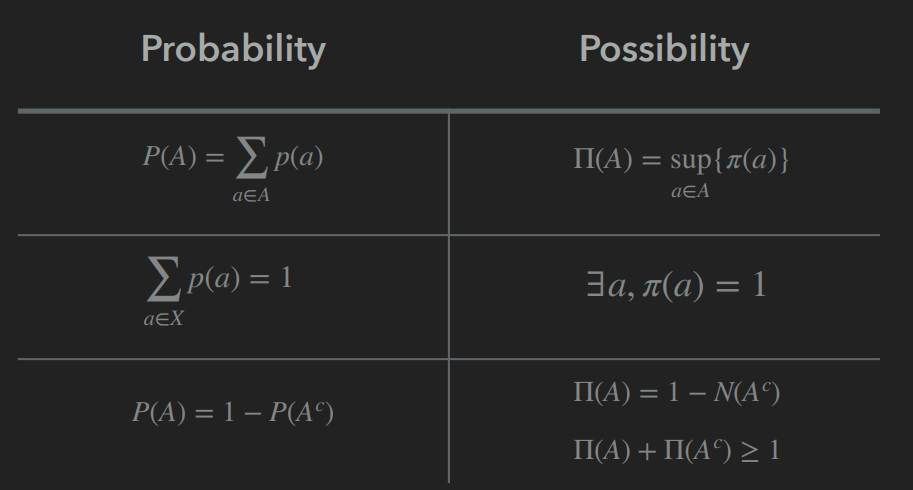
\includegraphics[width=0.5\textwidth]{img/sistemi_incerti/diff_prob_poss.png}
\end{figure}

Un caso particolare sono le funzioni booleane, funzione caratteristica di un insieme
ma che specificaun assegnamento di verità parziale. Quindi posso vedere un assegnamento 
parziale come un ortocoppia.

Posso vedere le belief function come un assegnamento di prob. agli insiemi, invece 
la probabilità è un assegnamento ad un evento.
\subsection{Belief function, Evidence theory and Dempster-Shafer}
Dalla capacità si deriva:
\begin{itemize}
    \item \textbf{probabilità}: capacità additiva
    \item \textbf{belieaf/plausibility function}
    \item \textbf{necessity/possibility}: capacità minitiva/massitiva
\end{itemize}

L'idea è di associare delle probabilità ad osservazioni incomplete e imprecise.
Il valore di verità deriva dall'insieme ma l'elemento esatto non lo si conosce.

\begin{definizione}[\textbf{Mass function}]
    Sia $X$ un insieme di esiti di esperimenti, sia $A\subseteq X$, possiamo associare
    ad un evento una \textbf{distribuzione di massa} $m:2^X\to [0,1]$ tale che:
    \begin{itemize}
        \item $m(\emptyset) = 0$
        \item $\sum_{A\subseteq X}m(A) = 1$
    \end{itemize}
\end{definizione}

Stiamo associando una distribuzione di probabilità agli insiemi

\begin{definizione}
    $A$ si chiama \textbf{focal set} se $m(A)>0$ 
\end{definizione}

\begin{nota}
    l'interpretazione della distribuzione ha un significato di un punto di vista 
    di tipo  epistemico ovvero si basa sulla nostra conoscenza soggettiva. Più precisamente $m(A)$ specifica che l'agente 
    conosce $x$ è in $A$. La massa può non essere monotona $A\subseteq B$ allora 
    $m(B)\le m(A) $ se l'agente è abbastanza sicuro che $x$ è in $A$. Se $m(X)=1$
    allora l'agente non sa niente. 
\end{nota}

Possiamo definire
\begin{definizione}[\textbf{Belief function}]
    La \textbf{belief function} $Bel:2^X\to [0,1]$ indica il totale della massa certa in $A$
    $$Bel(A) = \sum_{B\subseteq A} m(B)$$
\end{definizione}
\begin{definizione}[\textbf{Plausibility function}]
    La \textbf{plausibility function} $Pl:2^X\to [0,1]$ indica il totale della massa possibile in $A$
    $$Pl(A) = \sum_{B\cap A \ne \emptyset} m(B)$$
\end{definizione} 

Abbiamo che $Bel\le Pl$ e sono duali ovvero $Pl(A) = 1- Bel(A^c)$.

\begin{nota}
    Ricorda che $m(\emptyset) = 0$
\end{nota}

Le distribuzioni di massa rappresentano la conoscienza a priori e le possiamo 
unire effettuando \textbf{dempster's rule}
\begin{definizione}
    Date $m1,m2$ distribuzini di massa:
    \begin{itemize}
        \item $m_{1,2}(\emptyset) = 0$
        \item $m_{1,2} (A) = \frac{1}{1-K}\sum_{B\cap C =A}m_1(B)m_2(C)$
        dove $K =\sum_{B\cap C =A}m_1(B)m_2(C)$ è la misura di conflitto.
    \end{itemize}
\end{definizione}

Questa regola va bene solo quando le distribuzioni di massa impongono dei vincoli
sulla situazione, predilige i punti in comune.

Esistono altre regole di aggregazione:
\begin{itemize}
    \item \textbf{non normalizzata}: $m_{1,2}(A) =\sum_{B\cap C =A}m_1(B)m_2(C)$
    \item \textbf{unione}: $m_{1,2} (A)=\sum_{B\cup C =A}m_1(B)m_2(C)$
\end{itemize}

Generalmente:
\begin{itemize}
    \item sotto l'ipotesi di mondo chiuso meglio la normalizzata
    \item sotto l'ipotesi di mondo aperto meglio la non normalizzata.
\end{itemize}

Se la distribuzione di maassa è sul singolo elemento e non sugli insiemi si ottiene 
la probabilità. Otteniamo invece la misura di necessità se i set focali sono uno incluso nell'altro.
Dalle belief si possono ottenere l'approssimazione rough se i focal set sono una partizione.
Quindi catturo rappresentazioni rough basate su relazione di equivalenza.

Per ora abbiamo visto solo misure quantitative, passiamo definire delle \textbf{misure qualitative}, 
in cui si associa quindi un valore da un insieme ordinato (ordine totale).

Dato un universo $X$, definiamo $\mu:2^X\to L$ dove $L$ è un insieme con ordine 
totale in cui gli elementi esprimono credenza.

\section{Misure di incertezza}
La misura principale per misurare l'incertezza è l'entropia e ne esistono di diverse 
tipologie.

$X$ è un insieme di possibili alternative con associate delle probabilità 
e solo una alternativa è possibile. Come possiamo quantificare il fatto che $x$ 
occorre? 
L'idea è di definire una funzione:
\begin{itemize}
    \item \textbf{decrescente}: più è probabile che 
    occorre $x$ allora meno entropia ha
    \item \textbf{additiva}: se $p(x,y) = p(x)\cdot p(y)$ allora 
    $$u(p(x,y)) = u(p(x)) + u(p(y))$$
\end{itemize}

Esistono diverse tipologie di entropia:
\begin{itemize}
    \item \textbf{Shannon}:  
    $$u(p(x)) = K\log_b(p(x))$$
    dove $b = 2$ se si rappresenta in $b$ mentre $-1$ per la normalizazione.
    L'incertezza associata ad un insieme è 
    $$H(X) = - \sum_{x\in X}p(x)\log_2(p(x))$$
    Questo misura il contenuto informativo atteso di $X$.

    \item \textbf{Ellerman}: misura il contenuto informativo di una partizione $\pi$.
    L'entropia è alta tanto quanto l'abilità di distinguere tra due alternative.
    Per esempio quando abbiamo una classe che include tutti gli elementi allora non 
    si ha l'abilità di distinguerli e quindi abbiamo poca informazione. Al contrario 
    quando abbiamo una classe di equivalenza per ogni elemento allora abbiamo 
    massima informazione.

    Il calcolo si basa sui \textbf{dits} (distinction): coppie ordinate $(u_i,u_j)$
    di elementi in blocchi differneti:
    $$dit(\pi) = \{(u_i,u_j)| u_i,u_j \text{ classi che riesco a distinguere }\pi\}$$
    $$H(\pi) = \frac{|dit(\pi)|}{|U\times U|}$$
    utile quando dobbiamo creare delle orthopartition.
\end{itemize}

Possiamo introdurre delle misure di entropia più generalizzate:
\begin{itemize}
    \item \textbf{fuzzy entropy}: dato un fuzzy $f:X\to [0,1]$  
    $$H(f) = -\sum_{x\in X }\left[ f(x)\log_2f(x) + (1-f(x))\log_2(1-f(x))\right]$$
    Misura il grado di fuzzyness, quando $h(f) = 0$ quando è un insieme booleano,
    altrimenti massimo quando $\forall x, f(x) = \frac{1}{2}$. Dati due fuzzy $f_1,f_2$
    allora l'entropia misura anche la relazione di fuzzyness ovvero $f_1\le f_2 \iff H(f_1)\le H(f_2)$
    \item \textbf{conflitto di evidenza}: misura quanto sono in conflitto due distribuzioni 
    di massa $m_1,m_2$. Due distribuzioni sono in conflitto se $m_1(A)\ne 0, m_2(B)\ne 0$ 
    $A\cap B=\emptyset$ allora 
    $$con(m_1,m_2) = -\log_2(1-K)$$
    dove $K=\sum_{A\cap B=\emptyset}^{m_2(A)\cdot m_2(B)}$ e $A,B$ sono insiemi 
    focali. Dove $con$ è monotona crescente rispetto a $K$:
    \begin{itemize}
        \item $con(m_1,m_2) = 0$ sse $m_1,m_2$ non sono totalmente in conflitto ($K=0$)
        \item $con(m_1,m_2) = \infty$ sse $m_1,m_2$ sono totalmente in conflitto ($K=1$)
    \end{itemize}
    Possiamo calcolare il conflitto all'interno di una distribuzione di massa $m$. Per 
    fare ciò dobbiamo specificare una distribuzione fittizia
    $$m_A(B) = \begin{cases}
        1 & B=A\\
        0&altrimenti
    \end{cases}$$
    La quantità di conflitto di un focal set  con tutti gli altri focal set è 
    $$con(m,m_A) = -\log_2(1-\sum_{B\cap A=\emptyset}m(B))=-\log_2Pl(A)$$
    Possiamo calcolare la media su tutti gli insiemi focali:
    $$E[m] = \sum_{A\in F}m(A)conn(m,m_A) = -\sum_{A\in F}m(A)\log_2Pl(A) $$
    con $F$ focal sets.
    Se $m$ è una distribuzione di probabilità quindi assegna una distribuzione 
    ai singoli elementi allora $E[m]$ è l'entropia di shannon.
    Il conflitto è anche chiamato \textbf{dissonance}. Se i focal set sono tutti 
    $$A_1\subseteq A_2 \subseteq \dots \subseteq A_n$$
    Allora $E[m]= 0$, possibilità e necessità è senza conflitto.
    \item \textbf{confusione di evidenza}: dal conflitto possiamo ottenere la confusione 
    usando $Bel$:
    $$C[m]=-\sum_{A\in F}m(A)\log_2Bel(A)$$
    Se $C[m]=0$ sse $m(A)=1$ per un particolare $A$ e $m(B)=0$ tutti gli altri.
    $C[m]$ caratterizza:
    \begin{itemize}
        \item più la distribuzione è uniforme allora più siamo confusi
        \item se conconcentriamo su un insieme focale allora la confusione è $0$.
    \end{itemize}
    \item \textbf{Ellerman} sulle orthopartition: Sia $\mathcal{O}$ una orthopartizione 
    allora $\sqcap_\mathcal{O}$ è l'insieme di tutte le partizioni consistenti con $\mathcal{O}$.
    quindi $\pi \in \sqcap_\mathcal{O}$ possiamo calcolare $H(\pi)$ (con quella di Ellerman) e successivamente 
    calcolare l'entropia della orthopartition:
    \begin{itemize}
        \item lower entropy:
        $$h_\ast(\mathcal{O}) = \min\{H(\pi)|\pi \in \sqcap_\mathcal{O}\}$$
        \item upper entropy:
        $$h^\ast(\mathcal{O}) = \max\{H(\pi)|\pi \in \sqcap_\mathcal{O}\}$$
        \item mean entropy:
        $$\hat{h}(\mathcal{O}) = \frac{h_\ast(\mathcal{O}) + h^\ast(\mathcal{O})}{2}$$
        \item avg entropy:
        $$h_A(\mathcal{O})= \frac{1}{|\sqcap_\mathcal{O}|}\sum_{\pi \in \sqcap_\mathcal{O}}H(\pi)$$
    \end{itemize}
    \item \textbf{Shannon} sulle orthopartition: abbiamo bisogno di una distribuzione 
    $p=\left[p_1,\dots,p_n\right]$ che sia compatibile con l'orthopartizione.
    $$\mathcal{P}_\mathcal{O} = \{\left[p_1,\dots, p_n\right] | p_i\in \left[\frac{|P_i|}{|U|},\frac{|P_i\cup Bnd_i|}{|U|}\right], \sum_{i=1}^{n}p_i=1\}$$
    \begin{itemize}
        \item lower entropy:
        $$h_{S\ast}(\mathcal{O}) = \min\{H_S(\pi)|\pi \in \sqcap_\mathcal{O}\}$$
        \item upper entropy:
        $$h_S^\ast(\mathcal{O}) = \max\{H_S(\pi)|\pi \in \sqcap_\mathcal{O}\}$$
        \item mean entropy:
        $$\hat{h}(\mathcal{O}) = \frac{h_{S\ast}(\mathcal{O}) + h_S^\ast(\mathcal{O})}{2}$$
        \item avg entropy:
        $$h_{SA}(\mathcal{O})= \frac{1}{|\sqcap_\mathcal{O}|}\sum_{\pi \in \sqcap_\mathcal{O}}H_S(\pi)$$
    \end{itemize}
\end{itemize}


Per valutare il soft clustering si usano le ortopartizioni e si applica l'entropia.
L'entropia mi rappresenta le possibili coppie ordinate che possiamo distinguere.

Il problema è che non è efficiente perché si entra nel combinatorio
e quindi spesso si usano delle euristiche. Oppure possiamo usare l'entropia di 
Ellerman che sono polinomiali.

Nelle orthopartizioni spesso si calcola la misura di mutua informazione, ovvero 
l'informazione comune tra due orthopartizioni. 

$$m(\mathcal{O}_1,\mathcal{O}_2) = h(\mathcal{O}_1) + h(\mathcal{O}_2) - h(\mathcal{O}_1\land \mathcal{O}_2) $$
Dove $h$ è una qualsiasi entropia definita e $\mathcal{O}_1\land \mathcal{O}_2$ è 
l'intersezione.

$$\mathcal{O}_1\land \mathcal{O}_2=\{O_{i1}\sqcap_t O_{j2}|O_{i1}\in \mathcal{O}_1 \land O_{j2}\in\mathcal{O}_2\}$$

dove $O_{i1}\sqcap_t O_{j2} = (L_1\cap L_2, U_1\cup U_2)$
L'intersezione si calcola con l'intersezione dell'approssimazione dal basso e l'unione del boundary. Si usa 
questa perché coincide con l'intersezione tra partizioni delle due orthocopie. Menomale che Silvio c'è!

\section{Unione sistemi incerti e sistemi complessi}
sistemi tempo discreto e spazio discreto e pazio finito. L'idea è di capire incertezza 
e complessità in ml.

Nella vita reale in sistemi complessi possiamo osservare solo una parte del mondo 
e tutto il resto è incerto.

\begin{definizione}[\textbf{Sistema dinamico deterministico}]
    Un \textbf{sistema dinamico deterministico} è una coppia $(X,f)$ tale che 
    $f:X\to X$  che seleziona lo stato successivo
\end{definizione}

Quando i sistemi dinamici sono non deterministici allora questo introduce incertezza,
perché la transizione determina diversi stati raggiungibili ma non si conosce
quello preciso.

\begin{definizione}[\textbf{Sistema dinamico non deterministico}]
    Un \textbf{sistema dinamico non deterministico} è una coppia $(X,f)$
    $(X,f)$, $f:X\to 2^X$  che seleziona un insieme di stati possibili successivi.
\end{definizione}

questo coincide col dire che lo stato successivo può essere uno dei tanti successivi,
perché quando abbiamo un'osservazione parziale allora passiamo avere diversi possibili 
stati successivi.

Per ogni sistema deterministico possiamo associare un grafo che mostra il passaggio 
da uno stato all'altro attraverso transizioni, questo mostra se si ha determinismo 
o meno. (formalismo per rappresentare un qualsiasi sistema dinamico a tempo discreto 
e a stato discreto) Per quelli continui si discretizza.


Reaction system modellano i processi chimici. Si formalizzano mediante $3$ insiemi di sostanze:
\begin{itemize}
    \item reagenti
    \item inibitori
    \item prodotti
\end{itemize}
La stessa sostanza può essere prima un reagente, poi un inibitore e poi un prodotto.
Poi abbiamo l'insieme delle reazioni, sono le regole che si chiamano reazioni.
Formalmente si descrivono $(S,A)$ $S$ sostanze $A$ regole. Le regole sono triple 
$(R\subset S, I\subset S, P\subset S)$ dove se $R=S$ e $I=\emptyset$ allora $P=R$.

\begin{esempio}
    $S=\{H,O,H_2O\}$ allora una regola è $R=\{H,O\}$ $I = \{\}$ $P=\{H_2O\}$.
\end{esempio}

\begin{esempio}
    Sia $S=\{A,B,C\}$ le regole possono essere:
    \begin{itemize}
        \item $(\emptyset, ABC,BC)$
        \item $(B, C,AB)$
        \item $(A, C,AB)$
        \item $(C, AB,AC)$
        \item $(AB, \emptyset,ABC)$
    \end{itemize}
    Tutte le regole vengono applicate in parallelo e quindi il risultato è l'unione 
    dei risultati di tutte le regole applicabili
\end{esempio}

Possiamo rappresentare anche le reti di petri.

Vogliamo modellare l'incertezza con un unico linguaggio per tutti i sistemi dinamici.

Un primo modo per modellarli universalmente è attraverso il grafo ma essendo semplice 
perdo informazioni.
\begin{definizione}[\textbf{pattern}]
\end{definizione}
Un pattern rappresenta un pezzo di informazione rispetto allo stato del sistema.
(in questo stato è presente una sostanza)
\begin{definizione}[\textbf{Spazio di pattern}]
    Lo \textbf{spazio di pattern} è una tripla $(P,\le, \sim_m)$ dove:
    \begin{itemize}
        \item $P$ è l'insieme di pattern
        \item $(P,\le)$ è un poset
        \item $\sim_m$ è una relazione di equivallenza sugli insiemi minimali di $P$
    \end{itemize}
    Deve valere che presi $p_1,p_2\in P$ tale che $p_1\sqcup p_2$ esiste sse $\exists
    p_1'\le p_1, p_2'\le p_2$ tale che $p_1'\sim_mp_2\implies p_1' = p_2'$.
\end{definizione}
La relazione d'ordine esprime il concetto di generalità mentre la relazione di equivalenza 
è sui pattern minimali ovvero quello specifico.


\begin{definizione}[\textbf{Pattern dynamical system}]
    \textbf{Pattern dynamical system} è una quindtupla 
    $$(X, f, \mathcal{P},g, h)$$
    dove:
    \begin{itemize}
        \item $(X,f)$ è un sistema dinamico
        \item $\mathcal{P} = (P, \le, \sim_m)$ è un pattern spece
        \item $h:X\to M$ dove $M$ è l'insieme di elementi massimali, la funzione 
        deve essere un isomorfismo (gli elementi massimali di descrivono lo stato)
        \item $g:X\to 2^P$ dove $g(x)$ è l'ideale principale in $h(x)$ (sono tutti 
        gli elementi che stanno sotto $h(x)$, ovverlo tutti elementi $\le h(x)$)
    \end{itemize}
\end{definizione}

Aggiungo più informazioni al sistema dinamico astratto ($(X,f)$)

\begin{esempio}
    Nei sistemi reattivi l'informazione è quale sostanza appartiene e quale no.
    Quindi $P=S\cup \overline{S}$, $S$ sono le sostanze che sono presenti e $\overline{S}$
    le sostanze assenti. Un pattern $p=\{a,b,\overline{c}\}$ non è detto che ci 
    siano tutte le sostanze. La relazione $\le$ è la relazione di specificità. Se 
    $p_1\subseteq p_2$ allora $p_1\le p_2$, ex: $\{a,b\}\le \{a,b,\overline{c}\}$.
    
    La relazione di equivalenza $\sim_m$ associa simboli simili ex: $a\sim_m \overline{a}$
    (ovvero la contraddizione). 

    Esiste un pattern join solo quando esistono 2 elementi minimali che sono esattamente
    uguali.

    $h(x)$ mapperà gli stati nei pattern più specifici, $h(ab) = ab\overline{c}$

    $g(x)$ rappresenta per ogni stato quali informazioni sono vere, ex: $g(ab)=a,b, \overline{c}, a\overline{c}\dots$.
\end{esempio}

Il tipo di incertezza che avremo sui sistemi dinamici coincide con l'applicazione 
di un test che mi da delle informazioni parziali sullo stato attuale e quello che 
ci interessa è trovare le sottoinformazioni dello stato scoperto che ci viene descitto 
dal testo.

\begin{definizione}
    Sia $$APDS= (X,f, \mathcal{P}, g,h,T)$$ ddove $T$ è un insieme di test che ci dicono 
    se dei pattern sono veri oppure no in un certo pattern.
\end{definizione}
\begin{definizione}
    Quuindi $t:\mathcal{P} \to \{T,F\}$ che restituisce true o false se il pattern 
    è presente nello stato oppure no. Il test deve essere:
    \begin{itemize}
        \item monotona crescente: $p_1\le p_2 \implies t(p_1)\le t(p_2)$
        Questo mi dice che $x:t(x)= \sqcup_{p\in g(x)} t(p)$
    \end{itemize}
\end{definizione}

Questi test introducono delle delle approssimazioni perché possono ritornare valori 
uguali per stati differenti. Questo mi porta a modellare l'incertezza come Roughset

Quindi dato un insieme di test $T$, abbiamo uno stato $x$ allora $[x]_T$ è la 
classe di equivalenza $x$ su un insieme di test $T$. Quindi possimao definire 
la routhapproximation di uno stato $x$ è $r(x) =(l(x), u(x))$ tale che 0
$$l(x) = \bigcap_{y\in [x]_T} g(y)$$
$$u(x) = \bigcup_{y\in [x]_T} g(y)$$

PEr un qualsiasi test possiamo calcolare il supporto ovvero l'insieme per cui il 
test è vero.

Dai test si ottengono le classi di equivalenza degli stati, dalle quali si ottiene 
la rough approx delle classi di equivalenza e quindi si può avere del sistema dinamico 
rappresentato come rough approx. Quindi si collassano gli stati nelle classi di 
equivalenza e nella rappresentazione con rough abbiamo la fraccia tra rough solo 
se esiste un arco da un nodo di una classe ad un'altra. Con questa trasformazione 
rischiamo di perdere il determinismo.

Possiamo avere un'altra incertezza dipendente dall'osservazione dell'evoluzione 
di uno stato
\begin{definizione}
    Un osservazione $O$ è una collezioni di cammini massimale (aciclico) 
\end{definizione}
Ogni cammino massimale è un'osservazioene.

Se introduciamo delle opprossimazioni allroa le osservazioni possono cambiare 
le osservazioni a causa dei test che creano un'approssimazione.

Ora ci interessa sapere se i test permettono di riconoscere il comportamento del 
sistema oppure se un test non è infomrativo, per fare ciò si sfruttano i Reduct.

Si rappresenta il sistema dinamico con l'information table, in questo modo Vogliamo
trovare il reduct dei test.

Dato un insieme di test  $T$ allora $F\subseteq T$:
\begin{itemize}
    \item $F$ è un superreduct totale (un super insieme di un reduct) è un reduct 
    senza la minimalità se non mi cambia il grafico della dinamica
    \item $F$ è un superreduct parziale se nel caso due stati appartengono alla calsse 
    di equivalenza allora possono rimanere così, se due stati non sono nella stessa classe 
    allora si preservano le stesse classi.
    \item $F$ è un superreduct locale la dinamica non cambia limitatamente all'osservazione
\end{itemize} 
Trovare un sup-reduct totale allora è polinomiale 

In un reaction sistem è Np-Hard perché è polinomiale nella dimensione del grafo 

In generale il reduct minimale è Np-completo.


\section{MLOps}
Si ha l'algoritmo di apprendimento, diamo in input un insieme di dati e una topologia della rete allora in output 
otterremo il modello con i parametri. Successivamente col modello effettueremo le predizioni.


Possiamo avere 2 tipi di incertezza:
\begin{itemize}
    \item sui dati di training: si effettua un campionamento dei dati reali che può essere schematizzato attraverso un 
    generatore di dati $\mathcal{D}$, questo contiene incertezza sui dati come bias, errori sui dati, missing o imprecisione.
    \item sui dati di predizioni: si vuole comunicare l'incertezza, ovvero dal momento che abbiamo in input incertezza allora vogliamo 
    quantizzare questa incertezza, stima della probabilità che la predizione sia corretta. (uncertanty quantification)
\end{itemize}





\section*{Uncertanty quantification nella classificazione (supervisionato)}

Abbiamo uno spazio $X$ (feature space) rappresentazione degli oggetti che voglio studiare. e poi si ha $Y$ che è il target space. EX:
$X$ insieme di immagini mentre $Y$ sono le etichette associate. Se $Y$ è numerabile allora è classifivazione (binaria) altrimenti se è almento la 
cardinalità del continuo allora si parla di regressione.

$\mathcal{D}(X, Y)$ è il data generation mekanism, ovvero $\mathcal{D}(X, Y)$ è la probabilià di pescare la coppia $X,Y$ se $\forall x \exists !y\mathcal{D}(x,y)=1$
allora è un problema deterministico, altrimenti no (ex: riconoscere una malattia man on bastano i sintomi per riconoscerla). Si assume 
che non valga il determinsmo.

Si denota $\mathcal{D}(X)=\mathcal{D}(y=!|x) = E[y|x]$ perché siamo in una distribuzione di bernulli quindi il valore atteso è la probabilità 
di pescare la classe positiva. $\mathcal{D}(X)$ è l'incertezza aleatorica ed è un'incertezza che non può essere eliminata perché è una caratteristica
del meccanismo di generazione dei dati ed è quella che vogliamo quantificare. 

Il problema è che non conosciamo perché se lo conoscessimo allora possiamo definire il \textbf{classificatore}
perfetto quinid $h(x)=E[y|x]$. noi ci vogliamo avvicinare il più possibile e quindi definiremo una loss $l:H\to \mathbb{R}$.
La più semplice è la zero loss  $z(h)-1$ ovvero $1-accuracy$ il problema di usare l'accuracy è che non c'è un'inica soluzione giusta 
perché non è una funzione convessa. Generalmente si usano altre funzioni di loss come $L_2$ (squared-error).

Noi vogliamo trovare un modello tale che 
$$\arg\max_h E_x[(h(x)-E[y!x])^2]$$
Ma noi possiamo approssimarlo con 

$$\arg\max_h E_{x,y}[(h(x)-y)^2]$$
perché vediamo le etichette dal dataset, inoltre possiamo approssimare il valore atteso con la media campionaria
$$\arg\max_h \frac{1}{2}\sum_{(x,y)}[(h(x)-y)^2]$$

e questo è un upperbound dell'errore vero effettivo.

Se il nostro errore è $\alpha$ allora il modello è $\alpha$-valido, l'obiettivo è trovare $0$-valido che è impossibile perché non 
conosciamo la distribuzione marginale. 

Un modo per calcolare $\alpha$ è approssimarlo, perché non possiamo calcolare correttamente perché ci servono tutti i dati,
$\alpha = |E_x[h(x)]-E_{x,y}[y]|$ che è $\alpha$-mean marginally consistant che mi specifica il la predizione media sulle etichette medie.
Questo non mi dice che il mio classificatore è quello corretto ma se non è $0$-mean marginally consistant allora non lo è sicuramente.
Possiamo ottenere da un modello il suo $0$-mean marginally consistant  allora sia $\Delta = E_{x,y}[y]-E_x[h(x)]$ allora posso 
definire $h'(x) = h(x) +\Delta$ che è $0$-mean marginally consistant perché correggo le predizioni con il suo errore. 

Per calcolarl oeffitivamente userò le medie campionarie al posto dei valori attesi ma è sempre un'approssimazione con errore $\sqrt{\frac{\log(1/\delta)}{2n}}\ge \alpha$ ($\alpha$ reale col valore atteso).
dove $n$ è la dimensione del dataset ma $\delta$ è la confidenza.

Il problema è che sto guardando le singole istanze ma le medie delle istanze.
Un modo migliore è la calibrazione

Supponiamo che per un'istanza $x$ il modello predice $p=h(x)$ noi lo interpretiamo come probabilità ma non sempre questo è vero.

Se $P(y=1|h(x)=p)= p$ allora il modello è calibrato allora possiamo interpretare come probabilità se $P(y=1|h(x)=p)\ne p$ allora 
il modello è scalibrato e $p$ non coicide con la probabilità (maggior parte delle volte). In generale si sovrastima le probabilità della 
classe negativa e si sottostima le probabilità della classe negativa.

Il predittore di bayes è calibrato quindi tutti modelli scalibrati allora non è il predittore corretto.

Dobbiamo capire se è possibile calcolare se il modello è calibrato e nel caso correggere la calibrazione (è possibile). Per farlo facciamo 
l'assunzione che l'insieme di tutti gli score che mi può dare è finito $|V=\{h(x), x\in X\}|<\infty$ e questo non è troppo restrittivo perché
su pc tutto è finito.

Si introducono 2 metriche $ECE$ (expected calibration error) 
$$ECE = \sum_{v\in V}P(h(x)=v)|v-E[y|h(x)=v]|$$
$$K_2 = \sum_{v\in V}P(h(x)=v)(v-E[y|h(x)=v])^2$$
Anche per queste metriche non si possono calcolare perché dobbiamo conoscere la distribuzione generatrice.

Possiamo sempre correggere l'errore di calibrazione attraverso un algo iterativo di $T$ step dove ad ogni step 
riduco l'errore, ad ogni step calcolo 
$$v^\ast = \arg\max_{v\in V}P(h(x)=v)|v-E[y|h(x)=v]|$$ 
e un altro ciclo for tale che $h(x)=v^\ast $ allora $h(x)=E[y|h(x)=v^\ast]$. 
In sostanza istanza per istanza correggo le prredizioni col valore corretto. Al limite si correggono tutti i valori.
LA probabilità e il valore atteso le calocliamo sul dataset per ottenere un upperbound. Il problema è che 
la complessità è molto elevata, esiste una versione senza il for su $T$, alla fine assicura la correttezza 
ma la complessità è sempre elevata per la cardinalità del dataset. Nella pratica si usa la tecnica 
di platt scaling che sfrutta un modello di machine learning che risolve un problema di regressione 
dove le feature sono $h(x)$ e l'output è $y$. Si risolve con la logistic regression,
ma non ha una certezza teorica sul risultato ma è più efficiente.
In questo caso il modello dipende dalle istanze, il problema è che si deve eseguire 
su dati mai visti ovvero su un (Calibration set).

Tornando al problema iniziale i modelli $h:X\to [0,1]$  si ha il problema che non 
è associato alla probabilità. Per risolverlo si può usare l'approccio di 
restituire $h_\tau :X\to 2^Y$ ovvero restituendo un insieme contenente la classe 
corretta con una certa confidenza (simile all'intervallo di confidenza). Si parla 
quindi di conformal prediction. Tutto si basa su test statistici.

Si parte dal modello costruito $h:X\to [0,1]$, si definisce una \textbf{conformity score}
function 
$$S:X\times \mathbb{Z} \to \mathbb{R}$$
\begin{esempio}
    $S(x,h) = |h(x)-y|$
\end{esempio}
Più alto è il valore di $S$ allora maggiore è l'errore sul'istanza. Avremo 
quindi un calibration set separato dal training set per cui calcoliamo per ogni
coppia $(x_1,y_1)\dot(x_n,y_n)$ calcoliamo $S_i$.

Definiamo un nuovo modello 
$$h'_\tau(x)=\{y\in Y, S(x,h)\le \delta\}$$
con $\delta = \tau$-quantile su $C$. 

Quindi in $C$ eisteranno un totale di $(1-\tau)(n-1)$ istanze tale che $S(x,h)\le \delta$.

L'idea è di identificare un insieme di etichette tale che con probabilità maggiore
di $1-\tau$ l'etichetta vera appartiene all'insiem ovvero 
$$P_{x,y}(y\not \in h'_\tau(x))\le \tau + \mathcal{O}(\frac{1}{n})$$
più grande è $\tau$ allora più è inutile.



\section*{Uncertanty quantification nel clustering (non supervisionato)}
\chapter{Sistemi incerti}
Si studieranno sistemi incerti che possono essere:
\begin{itemize}
    \item interpretazione dei testi
    \item incertezza dei mercati
    \item valutare il valore degli oggetti
    \item valutare un rischio
    \item prendere decisioni, l'incertezza può avere un'accezione positiva
    \item etc$\dots$
\end{itemize}

Lo studio dell'incertezza è fondamentale in machine learning, dal momento che 
gli algoritmi hanno bisogno di dati e questi possono avere un certo livello di 
incertezza. Fondamentale sarà capire:
\begin{itemize}
    \item l'\textbf{oggetto} dell'incertezza e la sua fonte
    \item il \textbf{livello} e la \textbf{magnitudine} dell'incertezza
    \item \textbf{come} comunicare l'incertezza, ovvero in che forma ed espressione
    \item \textbf{preché} comunicare l'incertezza, ovvero lo scopo di questa comunicazione
\end{itemize}

\begin{definizione}
    L'\textbf{incertezza}  è l'imperfezione dell'informazione dovuta a diverse cause
\end{definizione}
\begin{definizione}
    \textbf{Agenti} sono i soggetti che esprimono l'incertezza
\end{definizione}
\begin{definizione}
    \textbf{Oggetti} sono gli oggetti su cui un agente esprime incertezza
\end{definizione}
\begin{definizione}
    \textbf{Proprietà} sono le proprietà dell'oggetto su cui un agente ha incertezza
\end{definizione}
Ogni agente ha un'opinione su una proprietà degli oggetti.

L'incertezza può essere dovuta principalemnte da:
\begin{itemize}
    \item \textbf{informazioni incomplete} dovuto a diverse cause:
    \begin{itemize}
        \item \textbf{valori mancanti}: ex: voglio stabilire se l'auto è gialla ma
        non conosco il colore dell'auto
        \item \textbf{valori imprecisi}: ex: l'auto ha tra i 10 e 15 anni ma non 
        conosco l'anno preciso
        \item \textbf{proprietà mancanti}: conosciamo i sintomi del paziente ma non 
        ho abbastanza sintomi per determinare l'incertezza. ex: nel caso prendessimo come oggetti i
        pazienti e come proprietà i sintomi, non possiamo sapere se un paziente 
        ha una particolare malattia se ha dei particolari sintomi.
    \end{itemize}
    \item \textbf{randomicità}: non possiamo stabilire la 
    veridicità di un'informazione, ex: domani piove (non è detto)
    \item  \textbf{vaghezza}/\textbf{gradualità}: ex: l'auto è veloce, cosa significa veloce?
    (dipende dal contesto)
    \item \textbf{informazione inaffidabile}: si possono avere informazioni
    contrastanti dovuti da agenti che hanno opinioni diverse, elementi a favore
    o contro ed esempi e controesempi. In aggiunta, si possono avere informazioni
    inaffidabili perché possiamo non avere la conpleta fiducia nei dati a disposizione.
    Ex: L'auto di Giulia è rossa o nera, sicuramente non è blu.
    \item \textbf{non affidabilità}: non abbiamo completa fiducia nei dati a disposizione.
\end{itemize}

Esistono diverse forme di incertezza e generalmente si classificano all'interno
di una tassonomia. Le classificaizoni si dividino in:
\begin{itemize}
    \item \textbf{scope}: il campo del sapere che copre quella classificazione
    \item \textbf{criteria}: sorgente dell'incertezza
\end{itemize}

Una tassonomia ha lo scopo di essere universale per raccogliere tutti i tipi di
incertezze indipendentemente dal particolare campo. Le tassonomie sono composte
da alberi i quali hanno sempre come radice \textbf{ignorance} (simula la non conoscienza),
nessuna classificazione appare in tutte le tipologie di tassonomie, ma al massimo in alcune e non 
nella stessa posizione, le tassonomie possono essere più specifiche e possono avere delle intersezioni.

Non esiste e non esisterà un unico modo per classificare l'incertezza e l'ignoranza, 
però sono utilili per essere studiati per analizzare le caratteristiche comuni.

Esistono anche tassonomie che sono legate ad un campo, ex: ecologia o ML. Per
queste tassonomie più piccolo è il dominio e più specifica è la terminologia della
classificazione. L'ontologia del dominio (semantica) può essere utile per capire dove l'incertezza
è e come azionarsi per gestirla. Quando costruiamo una classificazione di dominio
deve essere chiara tutte le parti di incertezza.

Le classificazioni sono utili per identificare l'incertezza per poi capire come 
gestirla. Le classificazioni generali tornano utili per specificare una prima classificazione 
specifica dell'incertezza nel mio dominio.

I criteri per definire una classificazione sono i seguenti:
\begin{itemize}
    \item \textbf{source}:  classificano in base alla sorgente (incertezza 
    sui dati e sugli utenti, temporale, spaziale e linguistica$\dots$)
    \item \textbf{manifestazione concrete}: classificano in base a cosa implica l'incertezza
    \item \textbf{personalità in cui risiede l'incertezza}: classifichiamo in base
    al punto di vista che vede l'incertezza
\end{itemize}

Possiamo avere classificazioni a più dimensioni, come matrici, e quindi sono più
complete e complesse. 

Essendoci diversi tipi di incertezza, si hanno diversi tipi di strumenti per 
modellare l'incertezza:
\begin{itemize}
    \item estensione della probabilità:
     \begin{itemize}
        \item Belief functions
        \item Imprecise probabilities
    \end{itemize}
    \item alternative alla probabilità:
    \begin{itemize}
        \item Possibility Theory/Logic
        \item Fuzzy Sets/Logic
        \item Modal Logic
        \item Interval Sets
        \item Rough Sets
    \end{itemize}
\end{itemize}

\section{Logica a tre valori di verità}
Spono logiche che introducono un terzo valore di verità che può assumere diversi 
significati in base a due caratteristiche:
\begin{itemize}
    \item ontologico (riguardano un qualcosa di vero): il valore può essere usato per assegnare sfumature di verità (mezzo vero)
    oppure si può assegnare un significato indefinito oppure per specificare il 
    concetto di irrilevante.
    \item epistemico (riguarda un problema di conoscienza): il valore può essere 
    usato per assegnare il valore unknown oppure può essere usato per specificare 
    inconsistenze  oppure per assegnare ad affermazioni che possono essere possibilmente 
    vere ma si scoprirà sono in futuro.
\end{itemize}


\section{Algebra booleana}
\begin{definizione}
    Una relazione d'ordine parziale $R$ è una relazione binaria:
    \begin{itemize}
        \item riflessiva
        \item antisimmetrica
        \item transitiva
    \end{itemize}
\end{definizione}

\begin{esempio}
    Possiamo definire delle relazioni d'ordine parziale per le funzioni caratteristiche 
    e una funzione è minore dell'altra se la prima mappa un sottoinsieme della seconda 
    funzione caratteristica.
\end{esempio}

Possiamo utilizzare il diagramma di Hasse è un diagramma che permette di rappresentare 
un insieme parzialmente ordinato senza esprimere la riflessività e transitività.

\begin{definizione}
    Dato un poset $ \langle\mathcal{P}, \le \rangle$, due elementi 
    $a,b\in \mathcal{P}$ si dicono \textbf{comparabili} sse $a\le b$ o $b\le a$. Altrimenti 
    si diranno \textbf{incomparabili}.
\end{definizione}

\begin{definizione}
    Data una relazione di ordine parziale $\le$ su un poset $\mathcal{P}$, se $\forall b,a\in \mathcal{P}$
    $a\le b$ o $b\le a$ e $b\ne a$ allora $\le$ è una \textbf{relazione di ordine parziale ristretta} e 
    si segnerà con $<$.
\end{definizione}

\begin{definizione}
    Data una relazione di ordine parziale $\le$ su un poset $\mathcal{P}$, se $\forall b,a\in \mathcal{P}$
    $a\le b$ o $b\le a$ allora $\le$ è una \textbf{relazione di ordine totale} (ovvero quando 
    tutti gli elementi sono comparabili)
\end{definizione}

Per rappresentare un poset possiamo utilizzare dei diagrammi di Hasse, ovvero diagrammi 
che mostrano le relazioni di antisimmetria, riflessività e transitività attraverso 
un ordine topologico e collegamenti non orientati.

\begin{definizione}
    Dato un Poset $\mathcal{P}$, definiremo $0\in \mathcal{P}$ il \textbf{minimo}
    se $\forall p \in \mathcal{P}\implies 0 \le p$ 
\end{definizione}
\begin{definizione}
    Dato un Poset $\mathcal{P}$, definiremo $1\in \mathcal{P}$ il \textbf{massimo}
    se $\forall p \in \mathcal{P}\implies p\le 1$ 
\end{definizione}

\begin{definizione}
    Un poset con un minimo e un massimo è un \textbf{poset limitato} e si scrive 
    $\langle \mathcal{P},\le , 0, 1\rangle$
\end{definizione}

\begin{nota}
    elemento minimo e massimo di un insieme parzialemente ordinato POSET non sempre 
    esistono
\end{nota}

\begin{definizione}
    Sia $S\ne \emptyset$ tale che $S\subseteq \mathcal{P}$, definiremo:
    \begin{itemize}
        \item $x\in \mathcal{P}$ \textbf{least upper bound} ($x=\sup(S)$, $x=\lor S$) sse:
        \begin{itemize}
            \item $\forall s\in S, s\le x$
            \item se $c\in \mathcal{P}$ soddisfa $s\le c,\forall s\in S$ allora $x\le c$
        \end{itemize}
        Se vale solo la prima condizione allora si dirà \textbf{upper bound} di $S$
        \item $y\in \mathcal{P}$ \textbf{greatest lower bound} ($y=\inf(S)$, $y=\land S$) sse:
        \begin{itemize}
            \item $\forall s\in S, y\le s$
            \item se $d\in \mathcal{P}$ soddisfa $d\le s,\forall s\in S$ allora $d\le y$
        \end{itemize}
        Se vale solo la prima condizione allora si dirà \textbf{lower bound} di $S$
    \end{itemize}
\end{definizione}

\begin{osservazione}
    Dato il poset $\langle \mathcal{P},\le\rangle$ allora:
    \begin{itemize}
        \item sia $Y\subseteq\mathcal{P}$ allora $\sup (Y)$ e $\inf (Y)$ se esistono
        sono unici
        \item sia $Y_1,Y_2\subseteq\mathcal{P}$ tale che $Y_1\le Y_2$ (ovvero tutti 
        gli elementi di $Y_1$ sono minori di tutti gli elementi di $Y_2$) allora entrambi
        $\inf(Y_1)$ e $\sup (Y_2)$ esistono, sono unici e $\inf(Y_1)\le \sup(Y_2)$
        \item sia $x\le y\iff x\land y = x \land x\lor y=y$ 
    \end{itemize}
\end{osservazione}

\begin{nota}
    Dato il poset $\langle \mathcal{P},\le\rangle$ che ha un $\lor \mathcal{P}$ e 
    un $\land\mathcal{P}$ e quindi è limitato, allora 
    $$\land\mathcal{P}\le x\le \lor \mathcal{P}, \forall x\in \mathcal{P}$$ 
\end{nota}


\begin{definizione}
    Un \textbf{reticolo} è un poset $\langle \mathcal{L}, \le \rangle$ tale che 
    $\forall x,y\in\mathcal{L}$ esiste il $\sup(\{x,y\})$ e $\inf(\{x,y\})$
\end{definizione}
nei reticoli il $\inf \equiv \text{meet}$ ($x\land y$) e  $\sup \equiv \text{join}$ ($x\lor y$)

Più precisamente si avrà:
\begin{itemize}
    \item $a\land b \le \{a,b\}$ e se $x\le  \{a,b\}\implies x\le a\land b$
    \item $\{a,b\} \le a\lor b$ e se $\{a,b\}\le x \implies a\lor b \le x$
\end{itemize}
\begin{definizione}
    Un \textbf{reticolo} è \textbf{completo} sse $\inf(S)$ e $\sup(S)$ esistono 
    sempre $\forall S \ne \emptyset \subseteq\mathcal{L}$
\end{definizione}

Il $\sup$ e l'$\inf$ nei reticoli possono essere visti come delle operazioni binarie
dal momento che esistono sempre generando la seguente struttura algebrica $\langle \mathcal{L}, \land,\lor \rangle$:
$$\land : \mathcal{L} \times \mathcal{L} \to \mathcal{L}, (x,y) \to x\land y :=\inf(\{x,y\})$$
$$\lor : \mathcal{L} \times \mathcal{L} \to \mathcal{L}, (x,y) \to x\lor y :=\sup(\{x,y\})$$


\begin{teorema}
    Dato il seguente reticolo $\langle \mathcal{L}, \le \rangle$ allora è associata 
    la struttura algebrica $\langle \mathcal{L}, \lor, \land\rangle$ che contiene le 
    operazioni di meet e join sul reticolo, allora le operazioni rispettano 
    le seguenti proprietà $\forall x,y,z\in \mathcal{L}$:
    \begin{itemize}
        \item \textbf{idempotenza}:
        $$x\land x = x \quad x\lor x = x$$ 
        \item \textbf{commutativa}:
        $$x\land y = y\land x \quad x\lor y = y\lor x$$ 
        \item \textbf{associativa}:
        $$x\land (y \land z) = (x \land y)\land z \quad x\lor (y \lor z) =( x\lor y)\lor z$$ 
        \item \textbf{assorbimento}:
        $$x\land (x \lor y) =x\quad x\lor (x \land y) =x$$  
        \item inoltre:
        $$x\le y \equiv x=x\land y\quad x\le y \equiv y=x\lor y$$ 
    \end{itemize} 
\end{teorema}

Possiamo partire da un insieme generico definire due operazioni che sono commutative associative 
e assorbimento, con queste operazioni possiamo definire un reticolo.

\begin{teorema}
    Data la seguente struttura algebrica $\langle \mathcal{L}, \lor, \land\rangle$
    dove:
    \begin{itemize}
        \item $\mathcal{L}\ne \emptyset$
        \item $\land$ e $\lor$ sono due operazioni su $\mathcal{L}$ commutative, 
        associative e con l'assorbimento
    \end{itemize}
    Se definiamo una relazione binaria $\le\subseteq \mathcal{L}\times \mathcal{L}$
    tale che 
    $$x\le y \iff y=x\lor y \equiv x\le y \iff x= x\land y$$
    allora $\langle \mathcal{L},\le\rangle$ è un reticolo tale che 
    $$x\lor y = \sup \{x,y\} \quad x\land y = \inf \{x,y\}$$
\end{teorema}

Quindi a partire da un reticolo poset possiamo formare una struttura algebrica alla quale 
sarà associato un reticolo che è lo stesso di quello di partenza. 

Al contrario da una struttura algebrica di un reticolo possiamo formare un reticolo 
il quale sarà effettivamente lo stesso del reticolo poset associato.

esistono reticoli che non sono distributivi e reticoli che sono distributivi.

\begin{nota}
    Sia $\langle \mathcal{L}, \lor, \land\rangle$ una struttura algebrica che formula 
    un reticolo allora:
    \begin{itemize}
        \item Se l'elemento neutro dell'operazione $\lor$ esiste (quindi $0$), allora 
        questo elemento è unico ed è il minimo elemento rispetto alla relazione $\le$.
        \item Se l'elemento neutro dell'operazione $\land$ esiste (quindi $1$), allora 
        questo elemento è unico ed è il massimo elemento rispetto alla relazione $\le$.
    \end{itemize}
\end{nota}

\begin{teorema}
    Sia $\langle \mathcal{L}, \le, 0\rangle$ un reticolo limitato inferiormente allora 
    $\lor$ rispetta le seguenti proprietà:
    \begin{itemize}
        \item \textbf{idempotenza}:
        $$ x\lor x = x$$ 
        \item \textbf{commutativa}:
        $$x\lor y = y\lor x$$ 
        \item \textbf{associativa}:
        $$x\lor (y \lor z) =( x\lor y)\lor z$$ 
        \item \textbf{elemento neutro}:
        $$x\lor 0 =x$$  
    \end{itemize}
    Quindi $\langle \mathcal{L}, \lor, 0\rangle$ è un monoide commmutativo. Sotto queste 
    ipotesi allora possiamo dire che dal monoide commutativo possiamo ottenere un 
    reticolo dove $0$ è l'elemento minimo.
\end{teorema}

\begin{definizione}
    Dati due reticoli $\mathcal{L}_1, \mathcal{L_2}$ sono detti isomorfi se esiste 
    una mappa biettiva $\phi:\mathcal{L}_1\times \mathcal{L}_2$ tale che 
    per un arbitrario $x,y\in \mathcal{L}_1$
    $$\phi(x\land_1 y) = \phi(x)\land_2\phi(y) \quad \phi(x\lor_1 y) = \phi(x)\lor_2\phi(y)$$
    Se $\phi$ è un isomorfismo di reticoli allora $\phi^{-1}$ è anch'esso un isomorfismo
    di reticoli. L'isomorfismo tra reticoli preserva anche l'ordinamento quindi è anche 
    un isomorfismo di poset.
\end{definizione}

\begin{definizione}
    Se $\mathcal{L}$ è un reticolo distributivo se le operazioni rispettano la proprietà
    distributiva:
    \begin{itemize}
        \item $\forall x,y,z\in \mathcal{L}, x\lor (y\land z)= (x\lor y) \land (x\lor z)$
        \item $\forall x,y,z\in \mathcal{L}, x\land (y\lor z)= (x\land y) \lor (x\land z)$
    \end{itemize}
\end{definizione}

\begin{teorema}
    Sia $\langle \mathcal{L}, \land, \lor \rangle$ una struttura algebrica e si ha:
    \begin{itemize}
        \item $\mathcal{L}\ne \emptyset$
        \item $\land$ e $\lor$ sono due operazioni binarie che soddisfano le seguenti 
        proprietà:
        \begin{itemize}
            \item $x=x\land(x\lor y)$
            \item $x\land (y\lor z) = (z\land x) \lor (y\land x)$
        \end{itemize}
    \end{itemize}
    Allora $\mathcal{L}$ è un reticolo distributivo.
\end{teorema}


\begin{definizione}
    Se $\mathcal{L}$ è un reticolo limitato, allora identifichiamo $y\in\mathcal{L}$
    il complemento di $x\in \mathcal{L}$ tale che 
    $$x\lor y = 1 \quad x\land y = 0$$
\end{definizione}
se $x$ è il complemento di $y$ allora $y$ è il complemento di $x$.
Inoltre $0\lor 1= 1$ e $0\land 1 = 0$.

Nei reticoli distribuiti il complemento di un elemento, se esiste, è unico. Per 
reticoli non distributivi allora la proprietà non è unica. 

\begin{definizione}
    Un reticolo booleano è una struttura $\langle \mathcal{B}, \land,\lor, ',0,1\rangle$ 
    dove:
    \begin{itemize}
        \item $\mathcal{B}$ è un insieme contenente due elementi distinti $1,0$.
        \item $\land$ e $\lor$ sono due operazionin binarie su $\mathcal{B}$ dove 
        la struttura algebrica $\langle \mathcal{B}, \land,\lor, 0,1\rangle$  è 
        un reticolo distribuito limitato dagli elementi $0,1$, quidni $\forall x\in \mathcal{B}$
        $0\le x\le 1$.
        \item $\forall x \in \mathcal{B}, \exists x'\in \mathcal{B}$ tale che 
        $x\land x' = 0$ e $x\lor x' = 1$, quindi $x'$ è il complemento.
    \end{itemize}
\end{definizione}

Quindi un'algebra booleana è un reticolo distribuito, complementabile e limitato.
Avremo quindi l'operazione di complemento ovvero $':\mathcal{B}\to \mathcal{B}$
 tale che restituisce l'elemento complemento che è unico.

\begin{esempio}
    Un reticolo booleano è la famosa tabella di verità dell'and e or, il complemento 
    è rappresentat dall'operazione complemneto.
\end{esempio}

\begin{definizione}
    Un'algebra booleana è una struttura $\langle \mathcal{B}, \land,\lor, ',0,1\rangle$ 
    dove:
    \begin{itemize}
        \item $\mathcal{B} = \{0,1\}$
        \item $\land$ e $\lor$ sono due operazioni binarie su $\mathcal{B}$
        \item $':\mathcal{B}\to \mathcal{B}$ è l'operazione di complemento
    \end{itemize}
    tale che $\forall x,y,z\in \mathcal{B}$ valgono i seguenti assiomi:
    \begin{itemize}
        \item $x\lor y = y\lor x \quad x\land y = y\land x $
        \item $x\land (y\lor z) = (x\land y) \lor (x\land z) \quad x\lor (y\land z) = (x\lor y) \land (x\lor z)$
        \item $x\lor 0 = x\quad x\land 1 = x$ 
        \item $x\lor x' = 1\quad x\land x' = 0$ 
    \end{itemize}
\end{definizione}

\begin{definizione}
    Un'algebra booleana può essere definita da una struttura $\langle \mathcal{B}, \land,\lor, ',0,1\rangle$ 
    tale che $\forall a,b,c\in \mathcal{B}$ valgono i seguenti assiomi:
    \begin{itemize}
        \item $a\land b = (a'\lor b')'$
        \item $a \lor b = b \lor a$
        \item $a\lor (b\lor c) = (a\lor b)\lor c$ 
        \item $(a\land b)\lor (a\land b') = a$ 
    \end{itemize}
\end{definizione}

\begin{teorema}
    Ogni algebra booleanda è possibile prova le  seguenti affermazioni:
    \begin{itemize}
        \item Proprietà del reticolo:
        \begin{itemize}
            \item \textbf{idempotenza}:
            $$x\land x = x \quad x\lor x = x$$ 
            \item \textbf{commutativa}:
            $$x\land y = y\land x \quad x\lor y = y\lor x$$ 
            \item \textbf{associativa}:
            $$x\land (y \land z) = (x \land y)\land z \quad x\lor (y \lor z) =( x\lor y)\lor z$$ 
            \item \textbf{assorbimento}:
            $$x\land (x \lor y) =x\quad x\lor (x \land y) =x$$  
        \end{itemize} 
        \item Proprietà distributive:
        \begin{itemize}
            \item $\forall x,y,z\in \mathcal{L}, x\lor (y\land z)= (x\lor y) \land (x\lor z)$
            \item $\forall x,y,z\in \mathcal{L}, x\land (y\lor z)= (x\land y) \lor (x\land z)$
        \end{itemize}
        \item Elementi neutri e unità:
        \begin{itemize}
            \item $x\lor 0 = x\quad x\lor 1 = 1$
            \item $x\land 0 = 0\quad x\land 1 =x$
        \end{itemize}
        \item condizioni di ortocomplementazione:
        \begin{itemize}
            \item \textbf{involuzione}: $(x')'= x$
            \item \textbf{leggi di De Morgan}: $(x\land y)' = x'\lor y' \quad (x\lor y)' = x'\land y'$
            \item $x\lor x' = 1$
            \item $x\land x' = 0$
        \end{itemize}

    \end{itemize}
\end{teorema}

\begin{definizione}
    Sia $\langle \mathcal{B}, \land,\lor\rangle$ una struttura algebrica dove:
    \begin{itemize}
        \item $\mathcal{L}\ne \emptyset$
        \item $\land$ e $\lor$ sono due operazioni su  $\mathcal{L}$ che soddisfano:
        \begin{itemize}
            \item $x= x\land (x\lor y)$
            \item $x\land (y\lor z) = (z\land x) \lor (y\land x)$
            \item $x\land(y\lor y') = x\lor(y\land y')$
        \end{itemize}
    \end{itemize}
    allora $\mathcal{L}$ è un reticolo booleano.
\end{definizione}


\begin{definizione}
    Date due algebre $\mathcal{B}_1$ e $\mathcal{B}_2$ sono isomorfe se esiste un
    isomorfismo tra reticoli $\phi:\mathcal{B}_1\to \mathcal{B}_2$ che preserva 
    l'elemento complemento, $\forall x\in \mathcal{B}_1, \phi(x') = \phi(x)'$
\end{definizione}

\begin{esempio}
L'esempio classico di algebra booleana è $0, 1$ e gli operatori saranno $\land, \lor,\lnot$.
In questa algebra si può definire $\implies$.
\end{esempio}

\section{Logica proposizionale booleana}
Per definire le logiche bisogna definire singolarmente la \textbf{sintassi} e 
\textbf{semantica}. Successivamente su queste bisogna definire un sistema deduttivo 
per poter effettuare inferenza nella nostra logica.

In generalem per definire la sintassi sobbiamo definire un \textbf{alfabeto} $\mathcal{A}$
e un insieme di formule $\mathcal{F}$ su di esso, più precisamente l'alfabeto sarà
$\mathcal{A} =\{V, L, U\}$ dove:
\begin{itemize}
    \item $V$ è un insieme infinito di variabili proposizionali
    \item $L\ne \emptyset$ è un insieme finito di connettivi logici unari e binari
    \item $U$ è un insieme di simboli ausiliari come le parentesi e la punteggiatura
\end{itemize}

Per una generica logica booleana possiamo pensare di definire l'alfabeto in questo modo
$$\mathcal{A} = \{\{p,q,r,s,\dots\}, \{\lnot, \land, \lor, \supset \}, \{(,),\top, \perp\}\}$$

Dall'alfabeto si definisce l'insieme di formule, spesso chiamate FbF perché definite 
in modo induttivo.

Nel caso generale le formule ben formate $\mathcal{F}$ saranno:
\begin{itemize}
    \item $\forall v\in V, v\in \mathcal{F}$
    \item $p,q\in FbF: \lnot p, p\land q, p\lor q, p \supset q\in \mathcal{F}$
    \item Nient'altro è una FbF
\end{itemize}

Definiremo $L= \langle \mathcal{A},\mathcal{F}\rangle$ il linguaggio della logica classica 
proposizionale booleana.

Per definire una \textbf{semantica} dobbiamo passare prima da una specifica 
su come interpretare una particolare variabile dell'alfabeto.

Per interpretare le variabili definiremo una mappa $v:V\to \mathcal{T}$ una funzione 
che associa una variabile ad un possibile valore di verità. L'interpretazione
verrà esotesa successivamente a tutte le formule $\mathcal{F}$, definendo la mappa 
$v^\ast:\mathcal{F}\to \mathcal{T}$ nel seguente modo:
\begin{itemize}
    \item $v^\ast(p) = v(p), \forall p\in V$
    \item $v^\ast(\lnot p) = v^\ast(p)', \forall p\in \mathcal{F}$
    \item $v^\ast(p\land q) = v^\ast(p) \land v^\ast(q), \forall p,q\in \mathcal{F}$
    \item $v^\ast(p\lor q) = v^\ast(p) \lor v^\ast(q), \forall p,q\in \mathcal{F}$
    \item $v^\ast(p\supset q) = v^\ast(p) \implies v^\ast(q), \forall p,q\in \mathcal{F}$
\end{itemize}

Dove $\lnot, \land, \lor, \supset$ coincidono con gli operatori dell'algebra booleana
$', \land, \lor, \implies$.

\begin{nota}
    Il valore di verità della formula dipende dal valore di verità delle singole componenti
    elementari e questa proprietà si chiama \textbf{truth-functionality}.
\end{nota}

Successivamente si deve definire il concetto di soddisfacibilità.

\begin{definizione} 
    Se $v$ è la funzione di valutazione per un linguaggio formale $L$, se $p\in \mathcal{F}$
    e $v(p) = 1$ allora $v$ \textbf{soddisfa} $p$, $v\vDash p$.
\end{definizione}

Se $v$ non soddisfa $p$ allora $v(p) = 0$ e si scrive $v\not\vDash p$.

Diremo che una formula $p$ è \textbf{soffisfacibile} se $\exists v$ interpretazione 
tale che $v\vDash p$. Diremo che una formula $p$ è una \textbf{tautologia} se $\forall v$ interpretazioni
tale che $v\vDash p$. Diremo che una formula $p$ è una \textbf{contraddizione} se $\forall v$ interpretazioni
tale che $v\not \vDash p$.

\begin{nota}
    Se la formula $p$ è una tautologia allora si può direttamente scrivere $\vDash p$.
\end{nota}

\begin{definizione} [\textbf{Sistema deduttivo}]
    Un \textbf{sistema deduttivo} è una tripla $\langle L, \mathcal{U}, \{r_1,\dots, r_k\}\rangle$
    dove:
    \begin{itemize}
        \item $L$ è il linguaggio formale
        \item $\mathcal{U}$ è l'insieme di assiomi (tautologie)
        \item $\{r_1,\dots, r_k\}$ sono le regole di inferenza.
    \end{itemize}
\end{definizione}

L'insieme di assiomi della logica booleana sono:
\begin{itemize}
    \item $p\supset (q \supset p)$
    \item $(p\supset (q \supset r))\supset ((p\supset q)\supset (p\supset r))$
    \item $\lnot p \supset(p\supset q)$
    \item $(p\supset q) \supset((\lnot p\supset q)\supset q)$
\end{itemize}

L'unica regola di inferenza sarà il \textbf{modus pones}
$$\frac{p,p\supset q}{q}$$

Ovviamente gli assiomi possono essere scritti anche secondo $\land,\lor$ dal momento 
che 
$$p\land q \equiv \lnot(p\supset \lnot q) \qquad p\lor q \equiv (p\supset q )\supset q$$

Inoltre si può utilizzare anche $\iff$ che coincide con
$$p\iff q \equiv (p\supset q) \land (q\supset p)$$


\begin{definizione} [\textbf{Deduzione}]
    Dato un sistema deduttivo, la \textbf{deduzione} di $q$ a partire da un insieme
    di proposizioni $A= (p_1,\dots, p_n)$ (premesse) è quando possiamo arrivare 
    dalle premesse alla formula $q$ utilizzando le regole di inferenza. In qìuesto 
    caso avremo 
    $$p_1,\dots p_n \vdash q \equiv A\vdash q$$
\end{definizione}

Il concetto di soddisfacibilità deriva dalla semantica mentre il concetto di 
deduzione deriva dalla sintassi.

\begin{definizione}
    Due formule $p,q$ sono logicamente equivalenti sse $p\vDash q$ e $q\vDash p$
    e le riscriviamo $p\equiv q$.
    
    $$p\equiv q \iff \forall v \begin{cases}
        v(p)=1 \implies v(q)=1\\
        v(q)=1 \implies v(p)=1\\
    \end{cases}$$
\end{definizione}
\begin{teorema}
    La sequenza $\langle \mathcal{F}, \land, \lor, \lnot, 0, 1\rangle$ è una 
    algebra booleana
\end{teorema}

\begin{teorema}
    Sia una formula $p$ è provabile nella logica bolleana, ex: $\vdash p$ sse 
    $p$ è una tautologia  nella logica, ovvero se $\forall v, v\vDash p$.
\end{teorema}


\section{Logiche a più valori di verità}

Logiche 3 valori di verità spesso assegnano un valore epistemico (sconosciuto) al
terzo valore di verità. Più spesso si l'interpretazione del terzo è una verità 
sfumata (mezzo vero), oppure per identificare un valore sconosciuto, oppure per 
identificare un valore irrilevante.

Il valore epistemico del terzo valore porta ad un problema di vero funzionale,
dove se $p=u$ ma anche $\lnot p =u$ quindi $p\land \lnot p$ dovrebbe essere falso 
e $p\lor p$ dovrebbe essere vero ma in realtà sono entrambi $u$.

\subsection{Logiche a $3$ valori di verità}
Formalmente nella logica booleana, i connettivi sono fissi, nel caso a $3$ valori di verità 
si possono definire diversi modi per specificare i connettivi. Nella logica a 
tre valori, il terzo valore può assumere $3$ diversi significati:
\begin{itemize}
    \item \textbf{mezzo vero} (logiche Fuzzy): dove specifica un livello intermedio di certezza
    \item \textbf{indefinito} (logica di Kleene): dove specifica il livello di 
    indefinito
    \item \textbf{irrilevante} (logica Priest): non è associato al contesto
\end{itemize}

Quando si considera il terzo valore di verità come un significato \textbf{epistemico}
allora assume una semantica:
\begin{itemize}
    \item \textbf{sconosciuto} nella logica di Kleene, nella quale si hanno problemi 
    di vero funzionalità
    \item \textbf{inconsistenza} specifica un valore per una preposizione che può
    non essere consistente (logiche paraconsistenti come logica di Prist)
    \item \textbf{possibile} la proposizione può assumere un valore di verità 
    nel futuro ma lo si determinerà solo successivamente.
\end{itemize}

Avendo $3$ valori possiamo definire per ogni logica dei connettivi in modo che questi 
siano coincidenti con delle operazioni matematice, in questo modo possiamo associare 
ai valori di verità dei numeri $\{0,\frac{1}{2},1\}$.

Quando vogliamo definire la \textbf{congiunzione} dobbiamo vincolare il fatto che 
che si deve comportare come quella booleana e deve essere \textbf{monotona}.

\begin{definizione}
    Una congiunzione a $3$ valori è una mappa $\ast:3\times 3\to 3$ tale che:
    \begin{itemize}
        \item \textbf{monotona a SX}: $x\le y$ allora $x\ast z\le y\ast z$ 
        \item \textbf{monotona a dX}: $x\le y$ allora $z\ast x\le z\ast y$ 
        \item \textbf{stesso comportamento del booleano}: $F\ast F=F\ast T = T\ast F = F$ e $T\ast T = T$
    \end{itemize}
    inoltre $u\ast F = F \ast u = F$
\end{definizione}

Questa definizione copre tutte le combinazioni di valori che si hanno per la congiunzione 
booleana, le uniche combinazioni che mancano sono quelle tra il valore $u$ e 
il valore $T$ che in base a come le scegliamo determiniamo una congiunzione diversa.

\begin{table}[!h]
    \centering
    \begin{tabular}{c|c|c|c}
        $\ast$ & F & u & T \\
        \hline
        F        & F & F & F \\
        u        & F &  &  \\
        T        & F &  & T
    \end{tabular}
\end{table}

In totale possiamo definire $14$ congiunzioni delle quali:
\begin{itemize}
    \item $6$ sono commutative 
    \item $5$ sono commuttative e associative
    \item $2$ sono $t$-norme
    \item $1$ è $u$-norma
\end{itemize}

Alcune congiunzioni hanno un nome e definiscono la logica associata:
\begin{itemize}
    \item \textbf{sette}: dove $u\ast u= T$, $u\ast T = T$ $T\ast u = T$. Inoltre 
    è commutativa e associativa.
    \item \textbf{quasi conjuction}: dove $u\ast u= u$, $u\ast T = T$ $T\ast u = T$. Inoltre 
    è una $u$-norma e rispetta le proprietà di commutatività e associatività.
    \item \textbf{Kleene}: dove $u\ast u= u$, $u\ast T = u$ $T\ast u = u$. Inoltre 
    è una $t$-norma e rispetta le proprietà di commutatività e associatività.
    \item \textbf{Bochvar external}: dove $u\ast u= F$, $u\ast T = F$ $T\ast u = F$.
    Inoltre rispetta le proprietà di commutatività e associatività.
    \item \textbf{Lukasiewicz}: dove $u\ast u= F$, $u\ast T = u$ $T\ast u = u$. Inoltre 
    è una $t$-norma e rispetta le proprietà di commutatività e associatività.
\end{itemize}

Con lo stesso ragionamento si possono definire diverse tipologie di $\implies$,
come al solito si richiede sempre che si comporti come quella booleana e che sia 
monotona.

\begin{definizione}
    Un implicazione è una mappa $\implies: 3\times 3 \to 3$ tale che:
    \begin{itemize}
        \item \textbf{monotona a SX}: $x\le y$ allora $x\implies z\le y\implies z$ 
        \item \textbf{monotona a dX}: $x\le y$ allora $z\implies x\le z\implies y$ 
        \item \textbf{stesso comportamento del booleano}: $F\implies F=T\implies T = T$ e $T\implies F = F$
    \end{itemize}
    inoltre deve rispettare:
    \begin{itemize}
        \item \textbf{left neutrality o border condition}:$T\implies x = x$
        \item \textbf{order property}:$x\implies y = T\iff x\le y$
    \end{itemize}
\end{definizione}

Questa definizione copre tutte le combinazioni di valori che si hanno per la congiunzione 
booleana, ma mancano tutti le altre combinazioni.

\begin{table}[!h]
    \centering
    \begin{tabular}{c|c|c|c}
        $\implies$ & F & u & T \\
        \hline
        F        & T & T & T \\
        u        &  &  & T \\
        T        & F &  & T
    \end{tabular}
\end{table}

Anche qui in base a come definiamo le combinazioni mancanti definiamo dei connettivi 
di una particolare logica a tre valori.

La \textbf{negazione} può essere definita usando l'implicazione, in generale 
$a':= a\implies 0$  e in base a come definiamo la negazione sul valore $u$ 
si definiscono $3$ diverse negazioni:
\begin{itemize}
    \item \textbf{intuistica}: $u' = 0 $
    \item \textbf{involutiva}: $u' = u $
    \item \textbf{paraconsistente}: $u' = 1 $
\end{itemize}

Posso definire gruppi di connettivi e relazioni tra i connettivi ovvero posso ottenere 
un operazione di un gruppo da un operazione di un altro gruppo.

Da $\land,\implies$ della logica di Lukasiewicz posso definire tutti i connettivi 
di tutte le altre logiche, inoltre possiamo tradurre tutte le implicazioni usando 
la logica modale.


\subsection{Logica di Kleene}
La logica di Kleene viene sviluppata dallo studio delle \textbf{funzioni parziali ricorsive},
ovvero $f:\mathbb{N}^n\to \mathbb{N}$ che sono definite su un $D\subseteq \mathbb{N}^n$.
Durante il loro studio Kleene definisce 2 tipologie di logiche:
\begin{itemize}
    \item \textbf{strong}: logica alla base della gestione del valore null in SQL,
    il terzo valore di verità assume la semantica di \textbf{unknown}.
    \item \textbf{weak}
\end{itemize} 

L'insieme dei valori di verità è $\{F,T,u\}$  quindi $T=\{t\}$, $F=\{f\}$
mentre $u=\{t,f\}$ dove $t,f$ sono i valori di verità della logica booleana data 
tutta la conoscienza nota.

Per definire i connettivi possiamo utilizzare le operazioni tra insiemi:
\begin{itemize}
    \item intersezione $\sqcap$ ovvero applica l'operatore booleano $\land$ su 
    tra tutte le coppie di valori di verità
    \item unione $\sqcup$ ovvero applica l'operatore booleano $\lor$ su 
    tra tutte le coppie di valori di verità
    \item negazione $'$ coincide con il complemento degli insiemi di valori di verità.
    \item implica $\implies$ ovvero coincide con la seguente formulazione 
    $A \implies B \equiv (\lnot A) \lor B \equiv A' \sqcup B $
\end{itemize}

\begin{esempio}
    Ecco un paio di esempi:
    \begin{itemize}
        \item $F\sqcap T = \{f\} \sqcap \{t\} = \{f\land t\} = \{f\} = F$ 
        \item $F\sqcap u = \{f\} \sqcap \{f,t\} = \{f\land t, f\land f\} = \{f, f\} =\{f\}= F$
        \item $T\sqcap u = \{t\} \sqcap \{f,t\} = \{t\land t, t\land f\} = \{f,t\} = u$
        \item $T\sqcup u = \{t\} \sqcup \{f,t\} = \{t\lor t, t\lor f\} = \{t,t\}= \{t\}= T$
        \item $F\sqcup u = \{f\} \sqcup \{f,t\} = \{f\lor t, f\lor f\} = \{f,t\}= u$
    \end{itemize}
\end{esempio}

Le tabelle di verità sono le seguenti.

\begin{table}[b]
    \centering
    \begin{subtable}[t]{0.49 \textwidth}
        \begin{tabular}{c|c|c|c}
            $\sqcap$ & F & u & T \\
            \hline
            F        & F & F & F \\
            u        & F & u & u \\
            T        & F & u & T
        \end{tabular}
    \end{subtable}
    \hspace{\fill}
    \begin{subtable}[t]{0.49 \textwidth}
        
        \begin{tabular}{c|c|c|c}
            $\sqcup$ & F & u & T \\
            \hline
            F        & F & u & T \\
            u        & u & u & T \\
            T        & T & T & T
        \end{tabular}
    \end{subtable}
    \bigskip

    \begin{subtable}[t]{0.49 \textwidth}
        \begin{tabular}{c|c}
            $'$& \\
            \hline
            F  & T \\
            u  & u \\
            T  & F 
        \end{tabular}
    \end{subtable}


    \begin{subtable}[t]{0.49 \textwidth}
        
        \begin{tabular}{c|c|c|c}
            $\implies$ & F & u & T \\
            \hline
            F        & T & T & T \\
            u        & u & u & T \\
            T        & F & u & T
        \end{tabular}
    \end{subtable}
    \bigskip
    
\end{table}


Vale il modus ponens ma non esistono tautologie perché se associamo ad ogni variabile 
della formula il valore sconosciuto allora i connettivi restituiscono sconosciuto.

Alla logica di Kleene possiamo sempre associare una struttura algebrica, prima 
però dobbiamo introdurre il \textbf{reticolo di de Morgan}.

\begin{definizione}[\textbf{Reticolo di De Morgan}]
    Il \textbf{reticolo di De Morgan} è $\langle L, \land, \lor,',0,1\rangle$ che è un reticolo limitato $0,1$
    dove $1=0'$ e l'operatore $'$ soddisfa solo:
    \begin{itemize}
        \item $a=a''$
        \item leggi di de Morgan: $a'\land b' = (a\lor b)'\qquad a'\lor b' = (a\land b)'$
    \end{itemize}
    (quindi non $b\lor b' = 1$ che vale per le algebre booleane)
    Se vale la distributività allora si parta di algebra di De Morgan.
\end{definizione}

\begin{nota}
    Nel reticolo di De Morgan i seguenti punti sono equivalenti:
    \begin{itemize}
        \item $a'\land b' = (a\lor b)'$
        \item $a'\lor b'= (a \land b)'$
        \item $a\le b \implies b'\le a'$
        \item $a'\le b' \implies b\le a$
    \end{itemize}
\end{nota}

\begin{definizione}[\textbf{Reticolo/algebra di Kleene}]
    Un \textbf{reticolo/algebra di Kleene} è un reticolo/algebra di De Morgan tale che 
    $$a\land a' \le b\lor b'$$
\end{definizione}
\begin{esempio}
    esistono reticoli di De Morgan che non sono di Kleene.
\end{esempio}

Successivamente dobbiamo definire il sistema deduttivo della logica, per la logica 
di Kleene non esistono più assiomi, ma si hanno solo le regole di inferenza.
Ciascuna regola rappresenta una proprietà della nostra logica:
\begin{itemize}
    \item $\frac{a\land b}{a}, \frac{a\land b}{b}$ e $\frac{a, b}{a\land b}$
    \item $\frac{a}{a\lor b}$
    \item $\frac{a\lor b}{b\lor a}$
    \item $\frac{a\lor a}{ a}$
    \item $\frac{a\lor (b\lor c)}{ (a\lor b)\lor c}$
    \item $\frac{a\lor (b\land c)}{ (a\lor b) \lor (a\lor c)}$
    \item $\frac{ (a\lor b) \lor (a\lor c)}{a\lor (b\land c)}$
    \item $\frac{ a\lor c}{\lnot \lnot a\lor c}$
    \item $\frac{ \lnot(a\lor b)\lor c}{(\lnot a\land \lnot b)\lor c}$
    \item $\frac{ \lnot(a\land b)\lor c}{(\lnot a\lor \lnot b)\lor c}$
    \item $\frac{\lnot \lnot a\lor c}{ a\lor c}$
    \item $\frac{(\lnot a\land \lnot b)\lor c}{ \lnot(a\lor b)\lor c}$
    \item $\frac{(\lnot a\lor \lnot b)\lor c}{ \lnot(a\land b)\lor c}$
    \item $\frac{a\lor (b\land \lnot b)}{ a}$
\end{itemize}
Le regole di inferenza esprimono tutte le proprietà della logica,  ex: distributività, doppia negazione.

Anche qui abbiamo l'inferenza sintattica ovvero $\Gamma \vdash p$ con $\Gamma \subseteq \mathcal{F}$
allora significa che $p$ si può derivare dell'insieme di formule $\Gamma$ mediante 
l'applicazione di regole di inferenza.

Questa algebra permette di modellare le query con null nei dbms relazionali.

Ai valori di verità possiamo associare dei valori reali $F=0, T=1,u=\frac{1}{2}$.
Questo mi permette di definire le operazioni con delle operazioni matematiche:
\begin{itemize}
    \item $a\land b = \min \{a,b\}$
    \item $a\lor b = \max \{a,b\}$
    \item $a' = 1-a$
    \item $a\implies b = \max \{1-a,b\}$
\end{itemize}

Questo è uno dei possibili modi per estendere all'intervallo $[0,1]$ le operazioni.
Il problema del verità funzionale è che si considera $u$ come coflitto tra il vero 
e falso ma non tra quello noto come vero e noto come falso. Altre logiche separano 
queste operazioni.  


\subsection{Logica di Priest}
Logica paraconsistente, permette di associare il valore $u$ quando si hanno inconsistenze.
Quindi in questo caso i valori di verità considerati come veri come $1,\frac{1}{2}$
la conseguenza è che si hanno tautologie, tutte le tautologie booleane vengono preservate 
però perdo il modus ponens.


\subsection{Logiche con valori infiniti}
Quello che abbiamo fino ad ora è prendere le logiche booleane $\{0,1\}$ e le abbiamo 
generalizzate a $\{0,\frac{1}{2},1\}$. Ora definiamo logiche che hanno valori di 
verità in $[0,1]$. I connettivi su queste logiche devono essere:
\begin{itemize}
    \item \textbf{conformi alla logica booleana} (ovvero che $\ast$ su 0,1 si comportano come nella logica)
    \item \textbf{rispettino vero funzionale} ovvero $p\ast q $ basta conoscere il valore di verità
    di $p,q$ quindi diverso dalle logiche modali che non hanno questa proprietà.
    \item congiunzione e disgiunzione \textbf{commutative, associative e monotone}.
    \item implicazione deve soddisfare una forma generalizzata di modus ponens.
\end{itemize}
\begin{definizione}
    definiremo $\land$ come una famiglia di operatori chiamati $t$-norme, sono operatori 
    binari 
    $$\ast : [0,1]\times [0,1]\to [0,1]$$
    Devono soddisfare le seguenti proprietà:
    \begin{itemize}
        \item \textbf{commutatività} $a\ast b = b\ast a$
        \item \textbf{associative} $a\ast (b\ast c) = (a\ast b)\ast c$
        \item \textbf{monotona a SX} $a\le b\implies a\ast c \le b\ast c,\forall c$.
        \item \textbf{elemento neutro}: $a\ast 1 = a$ e $0\ast 1 = 0$
    \end{itemize}        
\end{definizione}

\begin{esempio}
    Esempio di operatori che soddisfano le condizioni e che hanno la semantica di 
    $\land$ sono:
    \begin{itemize}
        \item godel: $min\{a,b\}$
        \item Lukasiewicz: $\max\{0,a+b-1\}$
        \item prodotto: $a\cdot b$ 
        \item prodotto drastico: $\begin{cases}
            0& a,b\in [0,1)\\
            \min\{a,b\}
        \end{cases}$ ($\max, \min$ hanno senso anche nella logica a $3$ valori)
    \end{itemize}
\end{esempio}

\begin{nota}
    ricorda che $\langle [0,1], \ast\rangle$ è un monoide con elemento neutro $1$. 
\end{nota}



\begin{definizione}
    definiremo $\lor$ come una famiglia di operatori chiamati $t$-conorme, sono operatori binari 
    $$+ : [0,1]\times [0,1]\to [0,1]$$
    Devono soddisfare le seguenti proprietà:
    \begin{itemize}
        \item \textbf{commutatività}: $a+ b = b+ a$
        \item \textbf{associative}: $a+ (b+ c) = (a+ b)+ c$
        \item \textbf{monotone a sinistra}: $a\le b\implies a+ c \le b+ c,\forall c$.
        \item \textbf{elemento neutro}: $a+ 0 = a$ e $0+ 1 = 1$
    \end{itemize}
\end{definizione}
\begin{teorema}
Data una $t$-norma $\ast$ possiamo definire $$a+b= 1-[(1-a)\ast (1-b)]$$ Questa è una 
$t$-conorma che è la duale della $t$-norma.
\end{teorema}
\begin{nota}
    Questa è una generalizzazione delle 
    proiorietà di De Morgan perché se definiamo $'$ come $x'= 1-x$ allora $a+b = (a'\ast  b')'$.    
\end{nota}


\begin{esempio}
    Le $t$-conorme duali delle logiche introdotte prima sono:
    \begin{itemize}
        \item \textbf{Godel}: $min\{a,b\} = \max\{a,b\}$
        \item \textbf{Lukasiewicz}: $a+b = \min\{1,a+b\}$
        \item \textbf{Prodotto}: $a+b = a+b-a\cdot b$ (somma probabilistica)
        \item \textbf{Prodotto drastico}: $a+b =\begin{cases}
            1& a,b\in (0,1]\\
            \max\{a,b\} & altrimenti
        \end{cases}$
    \end{itemize} 
\end{esempio}

\begin{definizione}
    Diremo $t$-norme \textbf{continue a sinistra} $\ast$ se $\forall (x_0,y_0)\in [0,1]^2$
    $$\forall \epsilon >0, \exists \delta >0, \forall (x,y)\in (x_0  -\delta, x_0] \times (y_0-\delta, y_0], x\ast y > x_0 \ast y_0 -\epsilon$$
\end{definizione}
\begin{definizione}
    Diremo $t$-norme \textbf{continue a destra} $\ast$ se $\forall (x_0,y_0)\in [0,1]^2$
    $$\forall \epsilon >0, \exists \delta >0, \forall (x,y)\in (x_0  -\delta, x_0] \times (y_0-\delta, y_0], x\ast y < x_0 \ast y_0 -\epsilon$$
\end{definizione}

\begin{esempio}
    Godel, Lukasiewicz, Prodotto sono continue a SX, mentre prdotto drastico no
    \begin{proof}
        $\epsilon =0.2$ $x_0=0.5$ $y_0=1$ $(x,y)=(0.5,1-\frac{\delta}{2})$

        $x\ast y = 0 > 0.5 - 0.2 = 0.3$
        Non è soddisfatta. 
    \end{proof}
\end{esempio}
\begin{definizione}
    Data un $\ast$ $t$-norma continua a SX allora definiremo $a\implies_\ast b$ come 
    $$\sup = \{x\in [0,1]:a\ast x \le b\}$$
\end{definizione}

\begin{esempio}
    Per ogni logica induciamo:
    \begin{itemize}
        \item \textbf{Godel}: $$\implies_G= \implies_\ast \begin{cases}
            1 & a\le b \text{ per a$\ast$ 1 = a}\\
            b & a >b
        \end{cases}$$ 
        \item \textbf{Lukasiewicz}: $$\implies_L = \min\{1,1-a+b\}$$
        \item \textbf{Goguen}: $$\implies_G =  \begin{cases}
            1 & a\le b\\
            b/a & a >b
        \end{cases}$$ 
    \end{itemize}

\end{esempio}

\begin{teorema}
    ogni implicazione definita generalmente coincide con  
    $$x\le (a\implies b ) \iff a\ast x \le b$$
    
\end{teorema}
Quando $x =1$ allora $1\le a\implies b \iff a\ast \le b$ 
allora $a\implies b = 1 \iff a\le b$. 

Il teorema può essere visto come la generalizzazione del modus ponens.
Se $a$ è vera con un certo grado $a$ e $(a\implies b)$ è vera con un grado $\ge x$ allora $b$ è vera almeno $a\ast x$. 

\begin{nota}
    impliczione è anche chiamata residuo della $t$-norma continua a SX
\end{nota}

Se la $t$-norma è continua allora possiamo definire le seguenti operazioni di reticolo
$$a\land b = a\ast (a\implies_\ast b)$$
$$a\lor b = ((a\implies_\ast b )\implies_\ast b)\land ((b\implies_\ast a) \implies_\ast a)$$

\begin{definizione}
    la negazione $'$ si può ottenere con $a\implies 0 \equiv \sup \{c\in [0,1]: a\ast c =0\}$.
    
\end{definizione}


\begin{esempio}
    Se consideriamo $\implies_L$ allora $a'= a\implies_L 0 = \min\{1,1-a\} = 1-a$ 
    coincide con la negazione standard.
\end{esempio}

$t$-conorma di Lukasiewicz $a \oplus b = \min \{1, a+b\}$ quindi $a\implies_L b = a'\oplus b$.

Come nel caso dei tre valori la Lukasiewicz può essere usata per definire gli operatori 
di tutte le logiche.

Vogliamo quindi definire una struttura algebrica che caratterizza le tnorme continue.

\begin{definizione}
    Un \textbf{reticolo residuato} è una struttura $\langle A, \land, \lor, \ast ,\implies,0,1\rangle$
    dove:
    \begin{itemize}
        \item $\langle A, \land, \lor, 0,1\rangle$ è un reticolo dove $0\le x \le 1 $ e 
        $a\le b \iff a\land b =a$
        \item $\langle A,\ast,1\rangle$ è un monoide dove $1$ è elemento neutro che rispetta 
        associatività e commutatività
        \item $a\le (a \implies b) \iff a \ast c \le b$, questa condizione può essere 
        sostituita anche da equazioni
    \end{itemize} 
\end{definizione}

Questa caratterizzazione non basta per caratterizzare tutte le $t$-norme, infatti 
per esempio le $t$-norme soddisfano questa prop. $(a\implies b )\lor (b\implies a) =1 $
non sono ricavabili dal reticolo residuato.

\begin{definizione} [MTL-algebra]
    La \textbf{MTL-algebra} è un reticolo residuato con l'aggiunta della condizione $(a\implies b )\lor (b\implies a) =1 $
\end{definizione}
MTL caratterizza le tnorme continue a sx

\begin{definizione}
    Chiamiamo $t$-algebra una MTL tale che $\langle [0,1], \min,\max,\ast,\implies, 0,1\rangle$
    dove:
    \begin{itemize}
        \item $\ast$ è t-norma conitnua a SX
        \item $\implies$ è il residuo che si ottiene dalla $t$-norma
    \end{itemize} 
\end{definizione}

\begin{teorema}
    Sia  $\phi, \xi$ due termini utilizzando i simboli di $mtl$-algebre.
    $\phi=\xi$ è soddisfatta in generale in una $MTL$-algebra sse è soddisfatta 
    in tutte le $t$-algebre.
\end{teorema}

Dalle MTL-algebre (T-norme continue a sx) posso aggiungere assiomi per definire:
\begin{itemize}
    \item $BL$-algebre dove le $t$-norme continue e devo aggiungere 
    $$a\land b = a\ast (a\implies b)$$
    \begin{itemize}
        \item se aggiungo $(a\implies 0 )\implies 0 = a\equiv [a''=a]$ è la $t$-algebra di Lukasiewicz 
        \item se aggiungo $a\ast a  = a$ è la $t$-algebra di Godel dove $\ast \equiv \land $ infatti $a\ast b = \min \{a,b\}$ 
    \end{itemize}
\end{itemize}

Dal punto di vista delle logiche abbiamo $\{0,1\}$ o $[0,1]$
oppure possiamo ragionare tramite insiemi $A$ e quindi possiamo pensare di usare la funzione
caratteristica di $A$ ($\xi_A: U \to \{0,1\}$).
Possiamo però generalizzare la funzione caratteristica in modo che restituisca un
valore $[0,1]$ che coindice con gli insiemi Fuzzy.

\section{Fuzzy set}
Permette di rappresentare l'appartenenza di un elemento ad un insieme con una 
percentuale di certezza. Per formalizzare questo concetto ci basta basarci sulla 
funzioen caratteristica degli insiemi. Di norma le funzioni caratteristiche sono 
definite in questo modo 
$$\xi_A: U \to \{0,1\}$$

Dove l'appartenenza è certa, sui quali possiamo effettuare delle operazioni insiemistiche 
come $\cup, \cap, ^c, \subseteq$ che si possono mappare sull'algebra booleana e quindi sulla 
logica booleana ($\lor, \land, ', \implies$).

Ora con i Fuzzy cambiamo la funzione caratteristica in questo modo
$$f_A: U \to [0,1]$$
Dove l'appartenenza ha un grado di confidenza, anche per questi insiemi possiamo 
applicare delle operazioni $\cup, \cap, ^c, \subseteq$ che si possono mappare 
sull'algebra MTL derivata dale logiche a più valori. Quindi si mapperanno nelle 
operazioni $t$-norme e $t$-conorme.

I fuzzy si possono rappresentare con dei grafici che esprimono gli elementi sull'asse 
$x$ e il grado di appartenenza agli insiemi sull'asse $y$ (\ref{fig:fuzzy_set}).

\begin{figure}[!h]
    \centering
    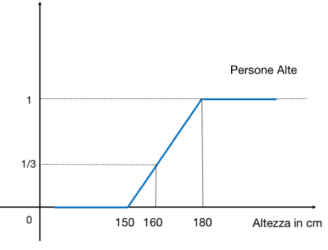
\includegraphics[width=0.5\textwidth]{img/sistemi_incerti/fuzzy.png}
    \caption{Esempio di rappresentazione grafica di un fuzzy set}
    \label{fig:fuzzy_set}
\end{figure}    
\begin{esempio}
    Insieme delle persone alte fino a $150$ si considera bassa,
    da $150$ a $180$ si può considerare medio alto e da $180$ è alto.
    La funzione potrebbe essere definita come 
    $$t(x) = \begin{cases}
        0& x\le 150\\
        \frac{x-150}{30}& 150\le x\le 180\\
        1& x\ge 180\\
    \end{cases}$$
\end{esempio}

I \textbf{fuzzy set}, a livello insiemistico, coincidono con l'insieme delle coppie 
elemento e grado di appartenenza. 

$$FS=\{(u, f(u)): u\in U, f(u)\in [0,1]\}$$

I \textbf{fuzzy set} possono essere \textbf{continui} o \textbf{discreti} se 
$U$ è \textbf{continuo} o \textbf{discreto}. Per gli insiemi continui ci sono alcune forme standard:
\begin{itemize}
    \item \textbf{triangolari}: dato $a<m<b$ allora sarà definito Così
    $$tr(x) = \begin{cases}
        0& x\le a\\
        \frac{x-a}{m-a} & x\in [a,m]\\
        \frac{b-x}{b-m} & x\in [m,b]\\
        0&x>b
    \end{cases}$$
    Usati nei Fuzzy control.
    \item \textbf{trapezioidali}: dati $a<m<n<b$ allora ho che da $[m,n]$ il grado
    di appartenenza che nel caso $m=n$ mi riconduco al triangolare
    \item \textbf{gaussiana}: dove
    $$g(x) = e^{-(\frac{(x-m)^2}{\sigma^2})}$$
    dove $m$ è il valore tipico 
\end{itemize}

\begin{definizione}
    Per un fuzzy set, l'insieme è \textbf{normale} se $\exists x, f(x) = 1$
\end{definizione}
\begin{definizione}
    Per un fuzzy set, il \textbf{support} è l'insieme tale che $\{x: f(x) >0\}$
\end{definizione}
\begin{definizione}
    Per un fuzzy set, il \textbf{core} è l'insieme tale che $\{x: f(x) =1\}$
\end{definizione}
\begin{definizione}
    Per un fuzzy set, $\alpha$-cut è l'insieme tale che $\alpha \in [0,1], \{x: f(x) \ge\alpha\}$
\end{definizione}
\begin{esempio}
    Dato un  $\alpha$-cut con $\alpha =1$ allora coincide con il sore set, mentre 
    quando $\alpha =0$ allora ottengo il support.
\end{esempio}

\begin{definizione}
    \textbf{strong} $\alpha$-cut è l'insieme tale che $\alpha \in [0,1], \{x: f(x) >\alpha\}$
\end{definizione}

I Fs sono degli insiemi e quindi possiamo definire le operazioni su insiemi $\cap, \cup, ^c, \subseteq$ 
partendo dagli insiemi normali quindi sulle funzioni caratteristiche, per poi 
mapparle sulle funzioni dei fuzzy:
\begin{itemize}
    \item \textbf{intersezione}: l'intesezione insiemistica classica 
    coincide con $(f\cap g)(x) = \min\{f(x), g(x)\}$ questo viene generalizzato dalle funzioni
    caratteristiche
    $$\mathcal{X}_A\cap \mathcal{X}_b = \begin{cases}
        1& \mathcal{X}_A(x) = 1\land \mathcal{X}_B(x)=1\\
        0& altrimenti
    \end{cases} \equiv 
    \min\{\mathcal{X}_A(x), \mathcal{X}_B(x)\}$$
    Quando siamo nel caso dei fuzzy set, $f(x), g(x) \in [0,1]$, allora $(f\cap g)(x)\in [0,1]$
    quindi coincide con la $t$-norma $(f\cap g)(x)= f(x) \ast g(x)$
    \item \textbf{unione}: l'unione insiemistica classica 
    coincide con $(f\cup g)(x) = \max\{f(x), g(x)\}$ questo viene generalizzato dalle funzioni
    caratteristiche
    $$\mathcal{X}_A\cup \mathcal{X}_b = \begin{cases}
        1& \mathcal{X}_A(x) = 1\lor \mathcal{X}_B(x)=1\\
        0& altrimenti
    \end{cases} \equiv 
    \max\{\mathcal{X}_A(x), \mathcal{X}_B(x)\}$$
    Quando siamo nel caso in cui $f(x), g(x) \in [0,1]$ allora $(f\cup g)(x)\in [0,1]$
    quindi coincide con la $t$-conorma $(f\cup g)(x)= f(x) + g(x)$ (coincide con $\max$)
    \item \textbf{complemento}: Quando siamo nel caso in cui $f(x), g(x) \in [0,1]$ allora $(f\cup g)(x)\in [0,1]$
    allora il complemento coincide con $1-f(x)$.
    \item \textbf{sottoinsieme}: nel caso delle funzioni caratteristiche 
     $\mathcal{X}_A\subseteq \mathcal{X}_B$
    è quando $\forall \mathcal{X}_A(x) \le \mathcal{X}_B(x)$ allora $f\subseteq g \iff \forall x, f(x)\le g(x)$.
    Questo può essere visto come l'operazione di $\implies$ infatti
    $$a\le b \iff a\implies b = 1$$

\end{itemize}

Abbiamo definito le operazioni in base alle $t$-norme e $t$-conorme, questo significa 
che possiamo definirle usano una delle varianti definite per la logica a valori 
infiniti.

\begin{esempio}
    Le varianti delle operazioni sono:
    \begin{itemize}
        \item $\min/\max$ (generalmente usata nei fuzzy)
        \item \textbf{Lukasiewicz} (l'intersezione nei fuzzy tende a schiacciare verso 0)
        \item \textbf{prodotto/somma probabilistica}
    \end{itemize}
\end{esempio}

Possiamo avere funzioni di aggregazione:
\begin{itemize}
    \item similarità: abbiamo il quasi associato alla proprietà
    \item incertezza: abbiamo il quasi associato al certamente. Teoria della possibilità 
    distribuzioni di possibilità
    \item preferenza:
\end{itemize}


\begin{definizione}[\textbf{Variabile linguistica}]
    In sostanza è una tupla $\langle L, T(L), G, U , M\rangle$ dove:
    \begin{itemize}
        \item $L$ è il nome della Variabile
        \item $T(L)$ insiemi di termini linguistici di $L$ ($L\in T(L)$) composto da 
        termini base e modificatori
        \item $G$ sono le regole con cui vando a mettere insieme i termini di base con i modificatori
        \item $U$ insieme universo, è il range dei valori che può assumere la variabile
        \item $M(x): U \to [0,1], \forall x\in T(L)$ assegna ad ogni termine un fuzzy set (dato un termine associanano un insieme fuzzy)
    \end{itemize} 
\end{definizione}

\begin{esempio}
    Un esempio può essere:
    \begin{itemize}
        \item $L=age$
        \item $G=linguistic_modifier+\{old, young\}$
        \item $T(L)=\{old,young, very_old,very_young, \dots\}$
        \item $U=[1,100]$
        \item $M(x):U\to [0,1], \forall x\in T(L)$, per esempio
        $$M(old)(u)=\begin{cases}
            \left[1+(\frac{u-50}{5})^{-2}\right]^{-1} & u\in [50,100]\\
            0 & u\in [0, 50)
        \end{cases}$$
        In questo caso si definisce $old$ da quando supera i $50$.
    \end{itemize}
\end{esempio}

Per assegnare una semantica numerica ai modificatori del linguaggio come tanto, molto,
poco, utilizziamo delle funzioni \textbf{modifier} che modifica l'incertezza di appartenenza degli 
elementi. La funzione sarà del tipo

$$m_A: [0,1]_A \to [0,1]_A$$

Le funzioni \textbf{modifier} si dividono in:
\begin{itemize}
    \item \textbf{concentration}: $con(f)(x)=[f(x)]^\beta, \beta>1$ da un significato di molto 
    quando il valore $\beta =2$. (concentro il fuzzy)
    \item \textbf{dilation}:  $dil(f)(x)=[f(x)]^\alpha, \alpha <1$ da un significato di abbastanza
    quando il valore $\alpha =\frac{1}{2}$. (allargo il fuzzy)
    \item \textbf{contrast intensifier}: modifica la confidenza degli elementi in modo 
    che si avvicini a $0$ o $1$ se rispettivamente $f(x)< 0.5$ e $f(x) >0.5$.
\end{itemize}

\begin{esempio}
    $vecchio(70)=0.94$ allora $molto_vecchio (70) = vecchio(70)^2$
    mentre $abbastanza_vecchio (70) = \sqrt{vecchio(70)}$
\end{esempio}

\begin{esempio}
    Per esempio un \textbf{contrast intensifier} definisce il modificatore $surely$
    attraverso le seguenti formule:
    $$sur(f)(x)=\begin{cases}
        2f^2(x) & f(x) \le 0.5\\
        1-2[1-f(x)]^2 & f(x) > 0.5
    \end{cases}$$
\end{esempio}

Ecco un immagine che mostra come si modifica la confidenza di un fuzzy utilizzando 
i modificatori (vedi \ref{fig:modificatori_fuzzy_set}).

\begin{figure}[!h]
    \centering
    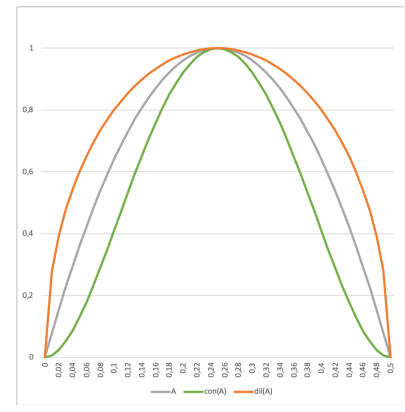
\includegraphics[width=0.5\textwidth]{img/sistemi_incerti/modificatori_fuzzy.png}
    \caption{Esempio di rappresentazione grafica di modificatori applicati ad un fuzzy set}
    \label{fig:modificatori_fuzzy_set}
\end{figure}  

Le variabili linguistiche permettono associare dei fuzzy set a dei concetti e 
mediante dei modificatori linguistici associare dei modificatori fuzzy per modificare 
la confidenza.

\subsection{Sistemi basati su regole}
I rules-based system sono sistemi specifici per dominio che usano delle regole 
per effettuare delle deduzioni o scelte.

I componenti base di questi sistemi sono (\ref{fig:rule-based}):
\begin{itemize}
    \item \textbf{base di conoscienza}: lista di regole di base che esprimono la 
    conoscenza del sistema nel dominio. L'espressione della base di conoscienza 
    si può fare attraverso due metodi:
    \begin{itemize}
        \item \textbf{mamdani}: regole if then con solo clausole formate da congiunzioni
        di espressioni boobleane in cui si testa il valore di alcune variabili linguistiche.
        \begin{center}
            IF ($X_1$ is $LT_1$) and \dots and ($X_n$ is $LT_n$) Then $Y$ is $LT_0$
        \end{center}
        Dove $X_i, Y$ sono variabili linguistiche e $LT_i$ sono i temini linguistici.
        \item  \textbf{sugeno}: cambiano le regole e permette di saltare il passo 
        di fuzzificazione.
        \begin{center}
            IF ($X_1$ is $LT_1$) and \dots and ($X_n$ is $LT_n$) Then $Y =p_0 + p_1X_1+ p_2X_2+\dots+ p_nX_n$
        \end{center}
        con $p=(p_0,\dots,p_n)$ vettore di numeri reali.
    \end{itemize}
    Essendo variabili linguistiche significa lavorare sui fuzzy.
    \item \textbf{inference engine}: effettua inferenza o prende decisioni in base alle interazioni 
    tra input e la base di conoscienza. Il processo di applicazione delle regole 
    si basa sui seguenti passi:
    \begin{itemize}
        \item \textbf{match}: si prende l'input si metcha con le regole, si possono 
        avere match multipli e ogni regola genera un risultato. Alla fine si avrà 
        un insieme di risultati chiamato \textbf{conflict set}.
        \item \textbf{conflict-resolution}: si agrega ciascun risultato del 
        \textbf{conflict set} in modo da ottenure un unico valore.
        \item \textbf{esegue}: ottenuto il valore attuale effettua l'azione 
        desiderata
    \end{itemize}
\end{itemize}

\begin{figure}
    \centering
    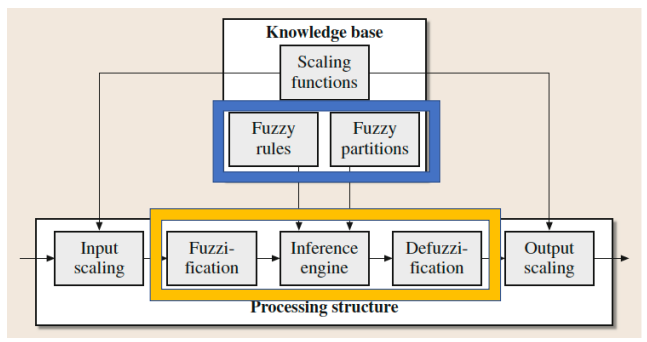
\includegraphics[width=0.5\textwidth]{img/sistemi_incerti/rule-based-system.png}
    \caption{Schema dei rule-based system}
    \label{fig:rule-based}
\end{figure}

Quindi dal mondo reale otteniamo un insieme di valori reali che descrivono 
la situazione, questi devono poi essere mappati sugli insiemi fuzzy associati (fuzzyficazione),
successivamente avendo i fuzzy si applica una regola alla volta, in modo da produrre 
un valore del fuzzy di output per ogni regola. Per produrre un valore di output 
per ogni regola, si applicano le $t$-norme e le $t$-conorme sui fuzzy delle regole 
in base ai connettivi. Quindi se abbiamo $m$ regole, otteniamo $m$ valori del 
fuzzy di output, quindi dovremo aggregarle, per fare ciò si usa la $t$-conorma ($\max$).

In questo modo otteniamo un unico valore di fuzzy in output, infine dobbiamo riconvertire
 il valore in numero reale e questo può essere vatto in due metodi:
\begin{itemize}
    \item \textbf{mean of maxima}: si estrae il valore 
    $$x^\ast = (a+b)/2$$
    dove $a = \inf\{x|B(x) = \max_y B(y)\}$ e  $b = \sup\{x|B(x) = \max_y B(y)\}$,
    ovvero coincide al valore medio dell'intervallo di valori di massima confidenza 
    del fuzzy di output ($B(x)$).
    \item \textbf{center of gravity}: si effettua una media pesata dei valori 
    del fuzzy per la loro confidenza
    $$x^\ast = \frac{\int_x x\cdot B(x)dx}{\int_x \cdot B(x)dx} \equiv x^\ast =\frac{\sum_x x\cdot B(x)dx}{\sum_x \cdot B(x)dx} $$
\end{itemize}

La parte di fuzzyficazione può essere fatta di due modi:
\begin{itemize}
    \item \textbf{FATI}: come spiegato prima, sia $B_i(y)$ il valore del fuzzy di 
    output dell'$i$-esima regola allora si calcola $B(y)= G(B_1(y),\dots, B_m(y))$
    ($G\equiv \max$) e poi inferisco il valore finale $Y_0=D(B(y))$ ($D\equiv$ center of 
    gravity o mean of maxima).
    \item \textbf{FITA}: per ogni regola ottengo $B_i(y)$ il valore del fuzzy di 
    output dell'$i$-esima regola allora effettuo subito l'inferenza per ogni 
    regola ottenendo il valore $y_i=D(B_i(y))$, infine aggrego i valori inferiti 
    pesandoli per la $t$-norma dei fuzzy di input $y=\frac{\sum y_i\cdot h_i}{\sum h_i}$
    dove $h_i=\ast(A_1(x_1),\dots,A_n(x_n))$.
\end{itemize}
\begin{nota}
Le regole possono essere attivate insieme e le posso rappresentare come una tabella 
se le regole sono poche.
\end{nota}

Spesso in output alle regole posso avere un singleton fuzzy ovvero quando abbiamo 
un unico valore a $1$ e tutto il resto a $0$ per ogni regola.

\section{Rough set}

Sono delle varianti di insiemi che permettono di effettuare operazioni di feature 
selection, Rough clustering e trovano applicazione anche ai sistemi dinamici.
I Rough set a livello generale sono degli insiemi di cui conosciamo con certezza 
solo alcuni elementi che appartengono e alcuni elementi che non appartengono, ma 
abbiamo elementi che forse appartengono o forse no.

\begin{definizione} [\textbf{information table} (information system)]
    L'\textbf{information table} $S(U) = \langle U, Att, Val, F\rangle$ dove:
    \begin{itemize}
        \item $U$ è un insieme di Oggetti
        \item $Att$ è un insieme di attributi
        \item $Val$ è un insieme di valori degli attributi
        \item $F:U\times A \to Val$ è una funzione che ad ogni oggetto ritorna il 
        valore dell'attributo scelto
        \item 
    \end{itemize}
\end{definizione}
\begin{esempio}
    Datta la seguente tabella informativa.
    \begin{figure}[!h]
        \centering
        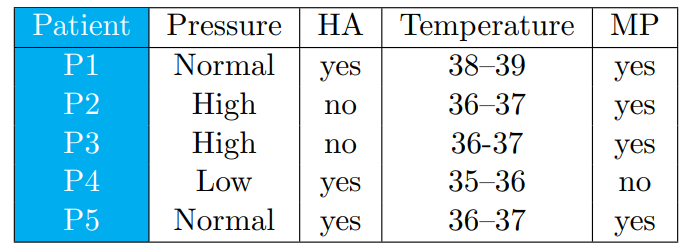
\includegraphics[width=0.5\textwidth]{img/sistemi_incerti/i_t.png}
    \end{figure}
    possiamo identificare:
    \begin{itemize}
        \item l'insieme degli oggetti $\{P_1,\dots,P_5\}$
        \item l'insieme degli attributi $\{Pressure, HA, Temperature,MP\}$
        \item l'insieme dei valori $\{Yes, No, 37-38,\dots\}$
        \item $F(P2, Pressure)=High$
    \end{itemize}
\end{esempio}
\begin{definizione}[\textbf{Decision system}]
    Un \textbf{decision system} $S(U) = \langle U, C\cup \{d\}, Val, F\rangle$ dove:
    \begin{itemize}
        \item $U$ è un insieme di Oggetti
        \item $C$ è un insieme di attributi dette condizioni
        \item $\{d\}$ è l'insieme di attributi di decisione
        \item $Val$ è un insieme di valori degli attributi
        \item $F:U\times C\cup \{d\} \to Val$ è una funzione che ad ogni oggetto ritorna il 
        valore dell'attributo scelto
        \item 
    \end{itemize}
\end{definizione}
In sostanza si aggiunge l'attributo decisione che corrisponde alla classe degli oggetti.
Possiamo raggruppare gli oggetti rispetto all'attributo decisione, questo mi permette 
di definire delle \textbf{classi di decisione} (insiemi $U_d = \{u\in U: F(u, decision) =d\}$) 

Il sistema viene definito:
\begin{itemize}
    \item \textbf{consistente}: se ogni coppia di oggetti che hanno attributi uguali 
    afferiscono alla stessa classe di decisione
    \item \textbf{inconsistente}: se esiste una  coppia di oggetti
    con attributi uguali e classi di decisione diverse
\end{itemize}

\begin{definizione} [\textbf{Relazione di Indiscernibilità}]
    Dato un sottoinsieme di attributi $A\subseteq Att$, due oggetti $x,y\in U$ sono 
    \textbf{indiscernibilità} rispetto a $A$ se 
    $$\forall a \in A, F(a, x) = F(a,y)$$
    Si scriverà $xI_A y$.
\end{definizione}
$I_A$ è una relazione di equivalenza perché è riflessiva, simmetrica e transitiva.
Questo significa che partiziona $U$ in classi di equivalenza chiamate anche \textbf{granularità 
delle informazioni}.
$$[x]_A:=\{y\in U:xI_Ay\}$$

\begin{definizione}[\textbf{Decisione generalizzata}]
    Una decisione generalizzata è una funzione decisione $\delta_A: U \to \mathcal{P}(Val)$
    tale che 
    $$\delta_A(x) = \{i \in Val: \exists y, xI_A y \land F(y,d) = i \}$$
\end{definizione}

La funzione di decisione generalizzata ritorna l'insieme delle decisioni di tutti 
gli oggetti che condividono gli stessi attrbuti dell'oggetto di input.

\begin{nota}
    Un sistema è \textbf{consistente} sse $|\delta_A(x)| = 1,\forall x\in U$.
\end{nota}

Data una partazione degli oggetti mediante l'indiscernibilità $\{P_1\}, \{P_2,P_3\}, 
\{P_4\}, \{P_5\}$, possiamo identificare un insieme normale $H = \{P_1\}\cup\{P_2,P_3\}$, 
che è certo, mentre possiamo definire $K=\{P_1,P_2\}$  che è un insieme \textbf{rough}
perché $P_2$ non conosciamo in che partizione si trova e infatti $K$ può essere approssimato 
tra due insiemi esatti (ovvero partizioni).
$$\{P_1\} \subseteq K \subseteq \{P_1,P_2,P_3\}$$


\begin{definizione}[\textbf{Approssimizzazioni}]
    Sia $S(U) = \langle U, Att, Val, F\rangle$ un information table. Dato un insieme 
    di attributi $A\subseteq Att$, allora per ogni $H\subseteq U$ definiamo:
    \begin{itemize}
        \item \textbf{lower approximation} di $H$:
        $$L(H):= \{x: [x]_A\subseteq H\}$$
        \item \textbf{upper approximation} di $H$:
        $$U(H):= \{x: [x]_A \cap H\ne \emptyset\}$$
    \end{itemize}
\end{definizione}

\begin{definizione}[\textbf{Rough}]
    La coppia $r(H) = \langle L(H), U(H)\rangle$ è chiamato \textbf{rough approximation} o
    \textbf{rough set}.
\end{definizione}
Ecco un esempio di rough set \ref*{fig:rs}.

\begin{figure}[!h]
    \centering
    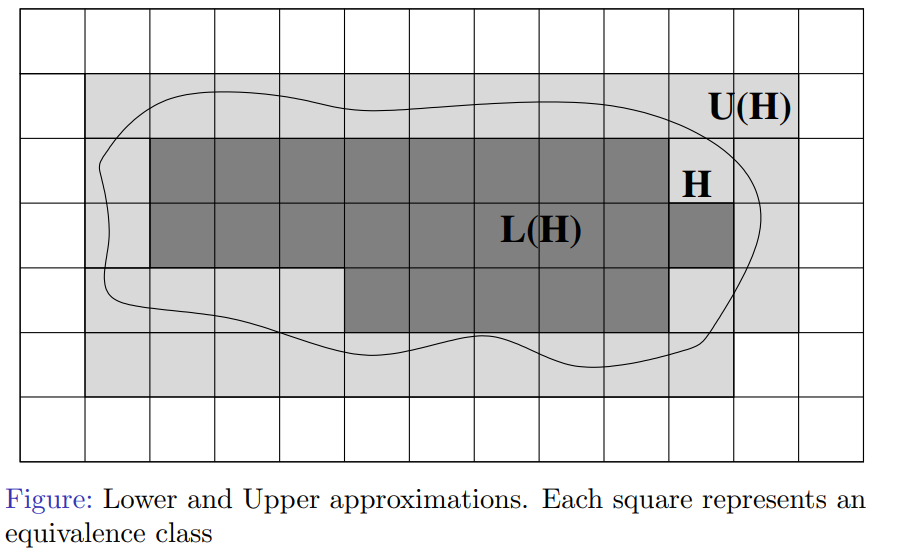
\includegraphics[width=0.5\textwidth]{img/sistemi_incerti/rs.png}
    \caption*{Esempio di Rough set}
    \label{fig:rs}
\end{figure}

Definiremo:
\begin{itemize}
    \item \textbf{esterior}: $E(H) = U^c(H), L(H)\cap E(H) = \emptyset$ ovvero gli 
    le classi che sicuramente non appartengono al rough
    \item \textbf{Boundary}: $Bnd(H) = U(H) - L(H)$ ovvero 
    le classi su cui abbiamo incertezza sull'appartenenza.
\end{itemize}

Possiamo misurare la grandezza del boyndary utilizzando le misure di incertezza:
\begin{itemize}
    \item \textbf{accuracy}: $\alpha(H) = \frac{|L(H)|}{|U(H)|}$
    \item \textbf{roughness}: $1-\alpha(H) = \frac{|Bnd(H)|}{|U(H)|}$
\end{itemize}

Le approssimazioni dall'alto e dal basso rispettano le seguenti proprietà:
\begin{itemize}
    \item $L(\emptyset)= \emptyset$, $L(U)=U$ uguale per l'approx alto
    \item $L(H)\subseteq H$ $H\subseteq U(H)$ 
    \item distributività $L(H\cap K)= L(H) \cap L(K) $, $L(H) \cup L(K) \subseteq L(H\cup K) $ contrario per l'approx alto
    \item monotonia $H\subseteq K\implies L(H)\subseteq L(K)$ uguale
    \item idempotenti $L(L(H)) = L(H)$ e $L(U(H)) = U(H)$
    \item dualità $L(H) = (U(H^c))^c$
\end{itemize}

\begin{nota}
    Queste sono proprietà tipiche di uno spazio topologico e sono operatori dipici
    delle logiche modali.        
\end{nota}

Fino ad ora abbiamo definito tutte i rough set tramite relazioni di equivalenza,
ma questo è troppo restrittivo, quindi possiamo generalizzare il ragionamento a una 
relazione $R$ "qualsiasi" (se $R$ è una relazione di equivalenza allora torno a prima). 
In realtà non possiamo estendere ad una $R$ binaria generica perché perdiamo 
alcune delle prorpietà introdotte prima. 
Definiamo una generica relazione $R\subseteq U\times U$, definiamo la granularità
dell'informazione $g_R(x) = \{y\in U: xR y\}$ allora otteniamo le seguenti approssimazioni
$$l_R(H) = \{x\in U:g_R(x)\subseteq U\}$$
$$u_R(H) = \{x\in U:g_R(x)\cap U = \emptyset\}$$

Si mantengono quindi le seguenti prorpietà per ogni $R$ scelta:
\begin{itemize}
    \item $l_R(U) = U$ 
    \item $u_R(\emptyset) = \emptyset$
    \item $l_R,u_R$ sono monotone
\end{itemize} 
Dobbiamo solo chiedere che $R$ rispetti:
\begin{itemize}
    \item \textbf{serialità} (no punti isolati): che ci aggiunge le proprietà $l_R(H) \subseteq u_R(H)$,
    $u_R(U) =U$ e $l_R(\emptyset) = \emptyset$.
    \item \textbf{riflessività}: che ci aggiunge le proprietà $l_R(H)\subseteq H \subseteq u_R(H)$
\end{itemize}

\begin{nota}
    se una relazione è \textbf{riflessiva} allora è anche \textbf{seriale}
\end{nota}

Se condidero rough set con $\mathcal{R}$ di similarità, sono certo che questa è simmetrica 
e riflessiva quindi perdiamo solo la transitività dalle relazioni di equivalenza.

Possiamo considerare i seguenti esempi:
\begin{itemize}
    \item $\mathcal{R}$ associata alla distanza tra oggetti utilizzabile quando 
    abbiamo piena conoscienza degli attributi degli oggetti
    \item $\mathcal{R}$ gestire valori mancanti
    $$x\mathcal{R}_Dy\iff \forall a_i\in D, F(x, a_i) = F(y,a_i) \lor F(x, a_i)=\ast \lor F(y, a_i)=\ast $$
    \item $\mathcal{R}$ gestire valori incompleti o parziali
    $$x\mathcal{R}_Dy\iff \forall a_i\in D, F(x, a_i) \cap F(y,a_i) \ne \emptyset$$
\end{itemize}

\subsection{Reduct}

I Rough set permettono di calcolare i reduct, ovvero gli insiemi di attributi più 
significativi per prendere una decisione e questi sono utili per definire delle 
regole per effettuare le decisioni a partire dal sottoinsieme di attributi.

Scelta la tabella, per calcolare i reduct posso calcolare la partizione degli oggetti 
eliminando ogni volta uno o più attributi, l'insieme di attributi minimo che preserva 
la partizione iniziale coincide con un \textbf{Reduct}. 

\begin{definizione}[\textbf{Reduct}]
    Sia $A\subseteq B\subseteq Att$, $A$ è un \textbf{reduct} di $B$ se :
    \begin{itemize}
        \item $\Pi_A = \Pi_B$
        \item $\not\exists C \subset A, \Pi_C=\Pi_B$
    \end{itemize}
    insieme minimale di attributi che mi rappresenta la stessa partizione (preservazione 
    della partizione e minimalità)
\end{definizione}
\begin{definizione}[\textbf{attributo indispensabile}]
    Sia $a \in A\subseteq Att$ è un \textbf{attributo indispensabile} in $A$ se $\Pi_A \ne \Pi_{A-\{a\}}$
\end{definizione}
\begin{definizione}[\textbf{Core}]
    Il \textbf{Core} è l'insieme indispensabile di attributi in $Att$ ovvero l'intersezione 
    di tutti i reduct in $Att$.
\end{definizione}

Dati $n$ attributi allora esistono $\mathcal{O} \left(\frac{3^n}{\sqrt{n}}\right)$ reduct.

Trovare il reduct più piccolo è più di NP completo e quindi una soluzione è parallelizzare 
oppure si devono utilizzare delle euristiche.


\subsection{Sistemi basati su regole}
Posso utilizzare i Rough set per i sistemi basati su regole. 

Se siamo nel caso di sistemi consistenti, dato un reduct allora si possono definire
delle regole in base ai valori che assumono gli attributi, in questo modo possiamo 
effettuare delle decisioni.

\begin{figure}[!h]
    \centering
    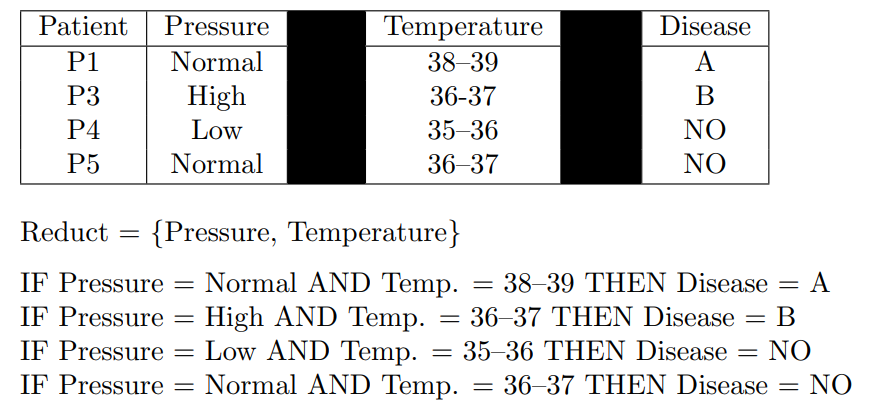
\includegraphics[width=0.5\textwidth]{img/sistemi_incerti/rule-based-system-rough.png}
\end{figure}

In caso di sistemi inconsistenti, il ragionamento cambia e non possiamo più basarci 
sulla \textbf{decisione} esata degli oggetti, bensì dobbiamo basarci sulla 
\textbf{decisione generalizzata}.

\begin{definizione}[\textbf{Estensione reduct alla decisione generalizzata}]
    Sia $A\subseteq B\subseteq Att$, $A$ è un \textbf{reduct} di $B$ se:
    \begin{itemize}
        \item $\delta_A = \delta_B$ (rimuovo inconsistenza)
        \item $\not\exists C \subset A, \delta_C=\delta_B$
    \end{itemize}
\end{definizione}

In questo modo risolvo l'inconsistenza a discapito di un'incertezza nelle regole,
infatti non ho una classificazione corretta, ma è sempre una classificazione ambigua ma senza errori.

\begin{figure}[!h]
    \centering
    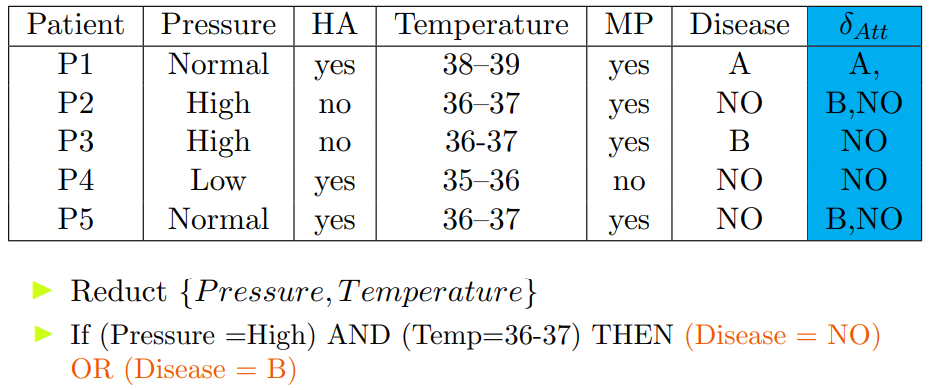
\includegraphics[width=0.5\textwidth]{img/sistemi_incerti/rule-based-system-rough-apr.png}
\end{figure}

Un altra soluzione all'inconsistenza del sistema  è valutare l'\textbf{indipendenza degli attributi}, 

\begin{definizione}[\textbf{Coefficiente di dipendenza}]
    sia $S(U)$ un decision system, sia $A\subseteq Att$ un insieme di attributi,
    $X_i$ le classi di decisione. Il \textbf{coefficiente di dipendenza} di decisione 
    $d$ dagli attributi $A$ è 
    $$Dip(A, d) = \frac{\sum |L_A(X_i)|}{|X|}$$

\end{definizione}

Il coefficiente specifica quanti oggetti riesco a caratterizzare con certezza per 
l'insieme di attributi $A$ sulla decisione $d$ ($Dip(A, d) =1$ è un sistema consistente). 

\begin{definizione}[\textbf{Estensione reduct al coefficiente di dipendenza}]
    sia $S(U)$ un decision system,  $A\subseteq B\subseteq Att$, $A$ è un \textbf{reduct} di $B$ se:
    \begin{itemize}
        \item $Dip(A,d) =Dip(B,d)$ (rimuovo inconsistenza)
        \item $\not\exists C \subset A, Dip(C,d) =Dip(B,d)$
    \end{itemize}
\end{definizione}

\begin{figure}[!h]
    \centering
    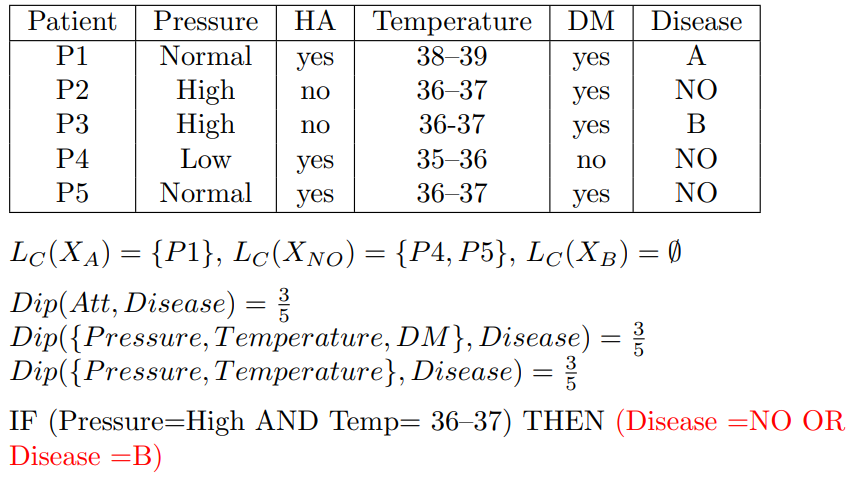
\includegraphics[width=0.5\textwidth]{img/sistemi_incerti/rule-based-system-rough-apr2.png}
\end{figure}

Un modo per alleggerire le varie richieste è quello di considerare reduct approssimati,
quindi non vado più a valutare attributi indispensabili/inutili, valuto quanto 
un attributo è significativo. 

Utilizziamo il coefficiente di dipendenza e valuto quanto 
varia il ocefficiente eliminando una porzione degli attributi.
$$Dip(C,d) = \frac{\sum_{min}^{max}|L_C(U_i)|}{|U|}$$
quindi ogni volta probo a rimuovere $B$ attributi e calcolo quanto varia il coefficiente
di dipendenza, se rimane sotto una soglia allora va bene altrimenti cerco nuovi 
attributi.
$$\frac{Dip(C,d)-Dip(C-B,d)}{Dip(C,d)} = \begin{cases}
    =0 & \text{def prec.}\\
    \le \epsilon 
\end{cases}$$

\begin{nota}
    In caso di attributi continui si fa una discretizzazione.
\end{nota}

Le regole le definiamo in questo modo 
$$r:U \to (d=v)$$
$match(r) = |U|$
$support(r) = |U\cap (d=v)|$
$consistenza = \frac{support(r)}{match(r)}$
$u$ oggetti.$(d= v)$ decisione uguale $v$

$r=(temp = 36-37)\to (D=no)$ in numero di oggetti che metchnano è $match(r)=3$ 
mentre $support(r)= 2$ quanti sono $no$ tra quelli che metchano.


\begin{esempio}
    Data la relazione $xI_Ay$ di discernibilità, abbiamo $n$ oggetti $|U|=n$ allora 
    dobbiamo definire una matrice $n\times n$ 
    $$c_{ij}= \{a\in A: F(a,x_i)\ne F(a,x_j)\}$$
    $A$ attributi.
$$
    \begin{array}{cccccc}
        x_U & a&b&c&d&e\\
        x_1 & 0&1&1&1&1\\
        x_2 & 1&1&0&1&0\\
        x_3 & 1&0&0&1&1\\
        x_4 & 1&0&0&1&0\\
        x_5 & 1&0&0&0&0\\
        x_6 &1&1&0&1&1\\
    \end{array}
    $$  
    La matrice di discernibilità è simmetrica e sulla diagonale $\emptyset$ e 
    $d_{ij}$ contiene di tutti gli attributi comuni a $x_i,x_j$.   
    $$
    \begin{array}{ccccccc}
        x_U & x_1 & x_2 & x_3 & x_4 & x_5 & x_6 \\
        x_1 & &1&1&1&1\\
        x_2 & \{a,d,e\}&1&0&1&0\\
        x_3 & \{a,c,d,e\}&0&0&1&1\\
        x_4 & 1&0&0&1&0\\
        x_5 & 1&0&0&0&0\\
        x_6 &1&1&0&1&1\\
    \end{array}
    $$

    Questa mi permette di ottenere il $core=\{a\in A: c_{ij}= \{a\}\}$

    Per calcolare i reduct: definsco una funzione booleana basandomi sula matrice 
    discernibilità composta da conciuzioni degli elementi $\lor c_{ij}$ 
    $$f(a,b,c,d,e,o)=(a\lor d\lor o)\land (a\lor d\lor c\lor e)$$

    and di tutte le entry della matrice di discernibilità, ogni entri coincide con un 
    or degli attributi. elimino le clasole contenenti elementi minimali

    $$f(a,b,c,d,e,o)= c\land e\land o \land (a\lor d)\land \dots$$
    La devo trasformare in forma normale disgiunta
    $$f(a,b,c,d,e,o)= (c\land e\land o \land a)\lor(c\land e\land o \land d)$$
    e questi sono tutti i reduct $c\land e\land o \land a$ e $c\land e\land o \land d$.
    Quello che abbiamo fatto è calcolcare gli implicanti primi della funzione booleana
    ovvero mi basta conoscere questi valori per decidere la tabella finale.
\end{esempio}

Abbiamo La matrice di discernibilità permette di avere un modo per calcolare i reduct 
attraverso la riduzione.
\subsection{Fuzzy Rough Set}
noi abbiamo fuzzy per rappresentare il vago e poi abbiamo Roughset che mi permette 
di suddividere gli oggetti, ovvero la granularità dell'universo (basati su insiemi e relazioni)
Possiamo unire i concetti usando fuzzy set e relazione fuzzy (quanto un elemento è
in relazione con un elemento). Per definire le approssimazioni si usano le $t$-norme 
e $t$-conorme (approssimo un insieme fuzzy attraverso due insiemi fuzzy).


\section{Orthopairs}
Sono la generalizzazione dei Roughset 
\begin{definizione}[\textbf{Orthopair}]
    L'\textbf{orthopair} è una coppia $(A,B)$ ortogonale o disgiunta di sottoinsiemi
    dell'insieme universo $X$: $A,B\subseteq X$ e $A\cap B=\emptyset$
\end{definizione}
\begin{definizione}[\textbf{Nested pairs}]
    L'\textbf{nested pairs} è una coppia $(A,C)$ equivalente all'ortopair tale che 
    $A\subseteq C \subseteq X$ e $C =B^c$
\end{definizione}

L'interpretazione associata all'orthopair $(P,N)$ è $P$ elementi positivi e $N$ 
elementi negativi.

Identifichiamo per l'orthopair il \textbf{boundary} $Bnd=(P\cup N )^c$ e quindi 
definiamo con un orthopair una \textbf{tripartition} dell'universo.

\begin{nota}
    $(P,Bnd)$ e $(N, Bnd)$ sono a loro volta delle orthopair perché sono insiemi disgiunti.
\end{nota}

\begin{esempio}
    Pari e dispari
    caso booleano insieme di variabili vere e false, in bnd è l'incertezza.
\end{esempio}

\begin{definizione}[\textbf{Consistenza}]
    Un insieme $S$ è \textbf{Consistente} con un'orthopair $O = (P,N)$ se 
    $$s\in P \implies x\in S\land x\in N \implies x\not \in S$$
\end{definizione}

\begin{esempio}
    Data l'ortocoppia $O=(\{1,3\}, \{2,4\})$ allora $S_1=\{1,3\}$ e $S_2=\{1,3,5\}$ 
    sono consistenti con $O$, al contrario $S_3=\{1,2,3,5\}$ e $S_4=\{1,5\}$ non sono 
    consistenti con $O$.
\end{esempio}

\begin{definizione}[\textbf{Disjoint}]
    Due orthopairs $O_1,O_2$ sono \textbf{disjoint} se:
    \begin{itemize}
        \item $P_1\cap P_2=\emptyset$
        \item $P_1\cap Bnd_2=\emptyset\land  Bnd_1\cap P_2=\emptyset$
    \end{itemize}
\end{definizione}

Possiamo ottenere delle orthopair a partire dai Roughset che possiamo vederli come 
$(L(H),U^c(H))$ o $(L(H),Bnd(H))$. Altrimenti possiamo tenerli da \textbf{modelli 
partziali}, ovvero si assegna un valore di verità per ogni elemento dell'insieme 
universo tale che sia consistente con l'orthopair. Questi modelli rispecchiano 
il significato di consistenza.
\begin{esempio}
    Sia $(P = \{x_1,x_4\},N =\{x_3\})$ allora possiamo pensare di avere i seguenti 
    modelli parziali:
    \begin{itemize}
        \item $v_1:= x_1=x_4=x_2 = true, x_3=false$
        \item $v_2:= x_1=x_4= true, x_3=x_2 =false$
    \end{itemize}
    Entrambi i modelli soddisfano l'orthopair, in generale tutti i modelli che 
    soddisfano l'orthopair sono quegli assegnamenti degli elementi tali che tutti 
    gli elementi di un insieme devono avere lo stesso valore ma diverso dagli elementi 
    dell'altro insieme. L'assegnamento agli elementi del boundary può essere fatto 
    come si vuole (incertezza). 
\end{esempio}

Le orthopair possono essere ottenute dai \textbf{Shadow set} che sono approssimazioni 
dei Fuzzy set mediante i valori $\{0, [0,1], 1\}$.

Infine gli orthopair possono essere ottenuti dalle \textbf{informazioni bipolari}
del mondo.

Esistono delle generalizzazioni delle orthopairs chiamate \textbf{Fuzzy orthopair} o \textbf{insiemi
fuzzy intuizionistici}. L'orthopair è una coppia di fuzzy $f_P,f_N:X\to \{0,1\}$
tale che $\forall x\in X, f_P(x)+f_N(x) \le 1$.

Un'altra generalizzazione è la \textbf{teoria della possibilità}, ovvero si ha un insieme 
di valutazioni $E$ arbitrarie, la classe dell'orthopair coincide  con la particolare 
classe \textbf{hyper-rectangular boolean possibility distributions} sullo spazio 
$\{0,1\}^n $.

Alle orthopair possiamo ritornare alle logiche a 3 valori. A partire da un universo 
$X$, si definisce $f: X \to \{0,\frac{1}{2},1\}$ tale che 
$$f(x) = \begin{cases}
    1&x\in A\\
    0&x\in B\\
    \frac{1}{2}&altrimenti\\
\end{cases}$$
Quindi possiamo definire una orthopair $(A_1,A_0)$ tale che 
$$A_1:=\{x:f(x)=1\} \qquad \text{dominio certo}$$
$$A_0:=\{x:f(x)=0\}\qquad \text{dominio impossibile}$$

In questo modo possiamo mappare i connettivi delle logiche a $3$ valori sulle orthopair 
o nestedpair.

\begin{figure}[!h]
    \centering
    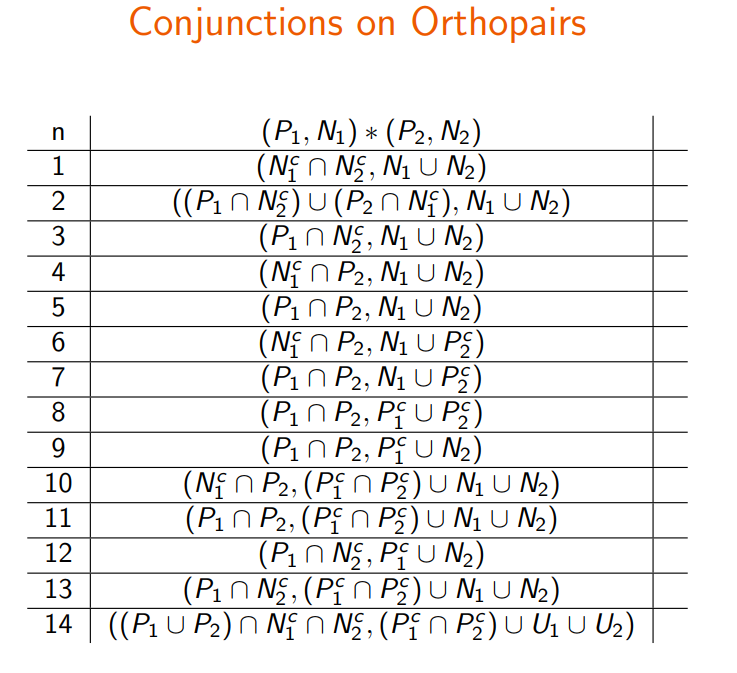
\includegraphics[width=0.5\textwidth]{img/sistemi_incerti/conj_ortho.png}
\end{figure}

\begin{figure}[!h]
    \centering
    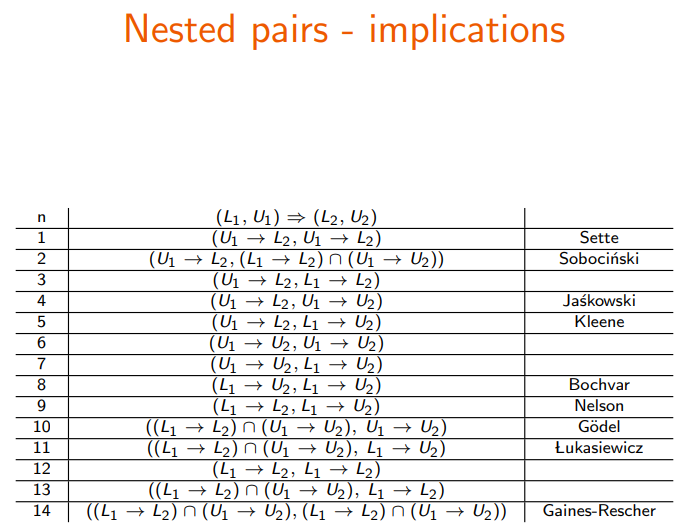
\includegraphics[width=0.5\textwidth]{img/sistemi_incerti/impl_nested_pair.png}
\end{figure}

Possiamo definire delle relazioni di ordinamento rispetto agli elementi dell'insieme 
universo in base ai valori di verità specificati dall'orthopair.

\begin{figure}[!h]
    \centering
    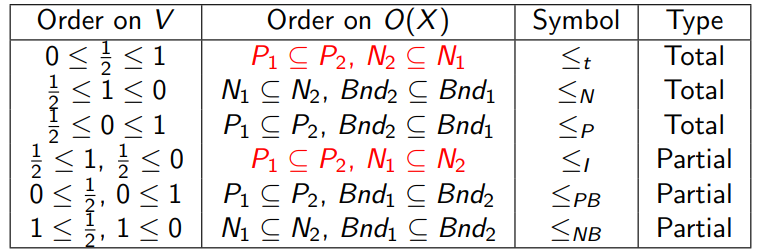
\includegraphics[width=0.5\textwidth]{img/sistemi_incerti/ordering.png}
\end{figure}

Possiamo identificare i seguenti ordinamenti importanti:
\begin{itemize}
    \item \textbf{ordine di verità} $O_1\le_t O_2$: $O_2$ è più vera rispetto $O_1$, ordine totale rispetto al valore di verità
    \item \textbf{ordine di conoscienza} $O_1\le_l O_2$: $O_2$ è più informativa rispetto $O_1$ (boundary più piccolo), ordine parziale rispetto all'incertezza
    in cui $0,1$ non sono confrontabili ma ci interessa solo il confronto tra l'incertezza
    e la certezza.
\end{itemize}

Definendo un ordinamento totale basato sui $3$ valori, possiamo derivare quindi delle operazioni 
di meet e join derivate dalle logiche a $3$ valori.

\begin{figure}[!h]
    \centering
    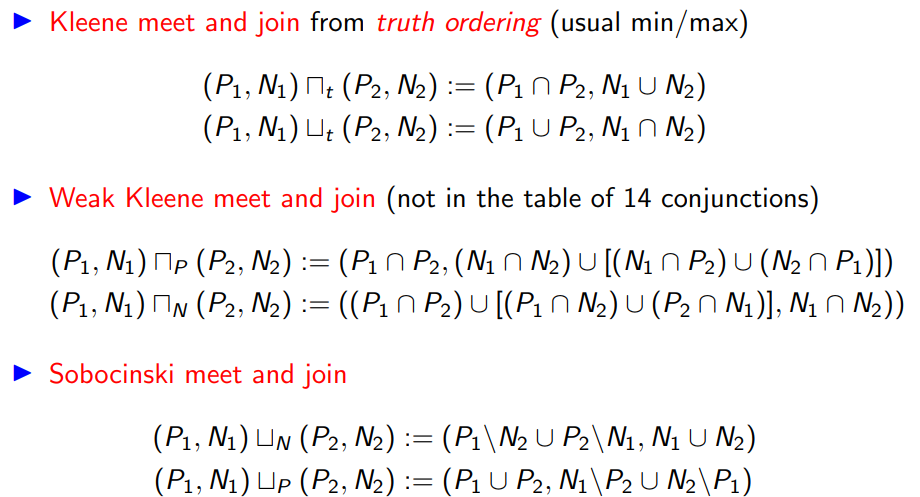
\includegraphics[width=0.5\textwidth]{img/sistemi_incerti/op_ortho.png}
\end{figure}


Definendo un ordinamento parziale basato sui $3$ valori, possiamo derivare quindi delle operazioni 
di meet e join derivate dalle logiche a $3$ valori, hanno senso solo quando si mantiene 
la consistenza delle orthocoppie, ovvero quando non si ocntraddicono.

\begin{figure}[!h]
    \centering
    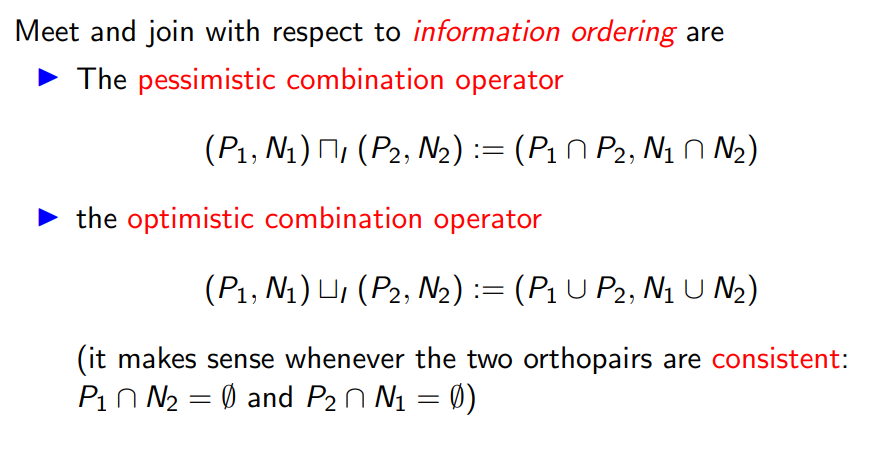
\includegraphics[width=0.5\textwidth]{img/sistemi_incerti/op_orthon_r.png}
\end{figure}

Si chiama operatore pessimistico perché prendo solo la conoscienza comune, mentre 
l'operatore ottimistico è un'operazione solo quando le ortocoppie sono consistenti e 
fa l'unione della conoscienza.

In aggiunta dal significato delle orthopair possiamo definire l'operatore di \textbf{consenso}
$$O_1 \odot O _2 = (O_1 \ominus O _2) \sqcup_l (O_2 \ominus O_1)$$
dove $O_1 \ominus O _2 :=  (P_1-P_2,N_1-N_2)$ è l'operatore di \textbf{differenza}.
L'operatore mi calcola ciò su cui sono d'accordo.
\begin{esempio}
    Sia $O_1=(\{x_1,x_2\},\{x_3,x_4\})$ con $x_1,x_2$ true e $x_3,x_4$ sono falsi.
    Sia $O_1=(\{x_1,x_3,x_4\},\{x_2,x_4,x_6\})$ con $x_1,x_3,x_4$ true e $x_2,x_4,x_6$ sono falsi.

    Allora $O_1 \odot O _2 = (\{x_1,x_5\},\{x_4,x_6\})$. 
\end{esempio}

Date due orthopair che rappresentano l'opinione di due agenti allora possiamo dire:
\begin{itemize}
    \item $\odot$: permette di ottenere l'accordo tra le due opinioni
    \item $\sqcap_l, \sqcup$: permettono di raggruppare le opinioni in modo pessimistico 
    o ottimistico
\end{itemize}

Nel caso di orthopair che rappresentano l'accettazione o il rigetto, le operazioni 
possono essere utilizzate per aggregare differenti decisioni. 

\begin{esempio}
    Queste operazioni permettono di unire risultati di classificazione.
    
\end{esempio}

I Roughset sono un sottoinsieme delle orthopair, infatti un generico $R(X)= (l(X), u(X))$ 
può essere associato ad un nestedpair e quindi un orthopair, perciò possiamo estendere 
tutte le operazioni sulle orthopair ai roughset.
Quindi possiamo combinare due Roughset usando le operazioni sulle orthopair che sono 
chiuse sui roughset. 

\begin{figure}[!h]
    \centering
    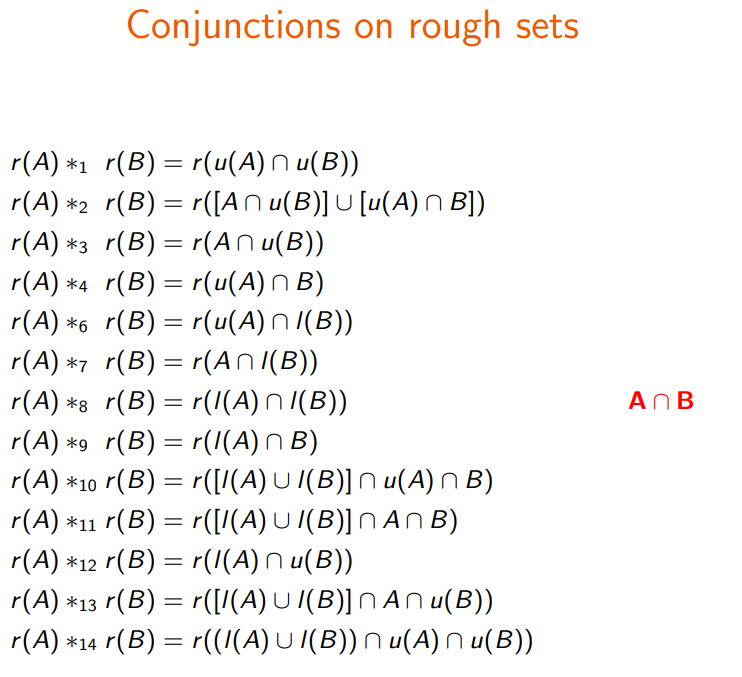
\includegraphics[width=0.5\textwidth]{img/sistemi_incerti/conj_RS.png}
\end{figure}

\begin{figure}[!h]
    \centering
    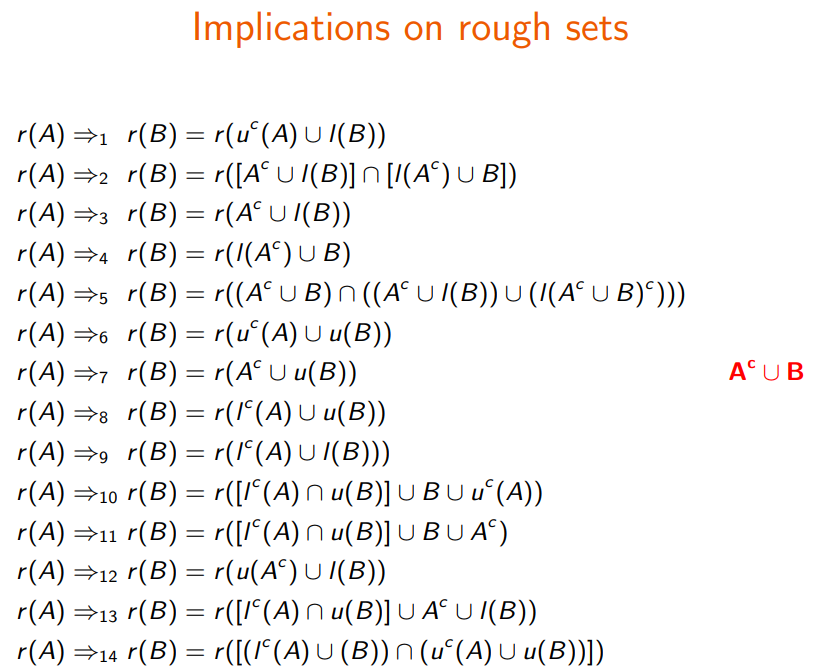
\includegraphics[width=0.5\textwidth]{img/sistemi_incerti/impl_RS.png}
\end{figure}

In generale dati due RS $r(A) = (l(A), u(A))$ e $r(B)=(l(B),u(B))$ allora si 
definisce l'unione e l'intersezione  come 
$$r(A)  \sqcap r(B) = (l(A)\cap l(B),u(A)\cap u(B))$$
$$r(A)  \sqcup r(B) = (l(A)\cup l(B),u(A)\cup u(B))$$

sappiamo che $r(A)  \sqcap r(B)$ e $r(A)  \sqcup r(B)$ sono proprio dei roughset,
supponiamo che siamo rispettivamente $r(C)$ e $r(D)$, in generale $C\ne A\cap B$ e $D\ne A\cup B$.

Per l'unione abbiamo diverse definizioni:
\begin{itemize}
    \item $C= [l(A)\cap l(B)] \cup Y$, $Y$ corrisponde ad un elemento scelto in una 
    classe di equivalenza, quindi si hanno diverse definizioni.
    \item $C=(A\cap B) \cup ((A\cap u(B))\cap(u(A\cap B)^c))$, in questo caso non 
    è simmetrica in $A,B$, quando $B=A^c$ allora $C\ne \emptyset$.
\end{itemize}

approssimazione C' è intersezione delle approssimazioni di A e B. La situazione è 
duale per $D$.

La scelta su come calcolare $C,D$ porta a dei problemi di interpretazione infatti 
abbiamo $2$ livelli di interpretazione:
\begin{itemize}
    \item linguaggio di insiemi (estensione): quando si lavora con le classi di equivalenza
    \item linguaggio di attributi (intensione): quando si lavora a livello di roughset
\end{itemize}
La soluzione dipende fortemente dalla partizione e dalle approssimazioni.

\begin{nota}
    $A\cap A^c \ne \emptyset$ 
\end{nota}

\section{Orthopartions}
Sono la rappresentazione incerta di classi di equivalenza

\begin{definizione}[\textbf{Orthopartition}]
    Una \textbf{orthopartition} è un insieme $\mathcal{O} = \{O_1,\dots, O_n\}$ di 
    orthopair tali che rispettano i seguenti assiomi:
    \begin{itemize}
        \item \textbf{disgiunzione}: $\forall O_i, O_j\in \mathcal{O}$ $O_i,O_j$ sono 
        disgiunte
        \item \textbf{copertura}: $\bigcap _i (P_i\cup Bnd_i) = U$
        \item \textbf{appartenenza a più boundary}: $\forall x\in U, (x\in Bnd_i) \implies (x\in Bnd_j), i\ne j$
    \end{itemize}
\end{definizione}

\begin{esempio}
    Sia $U=\{1,2,\dots,10\}$ la collezione $\{O_1,O_2,O_3\}$ è una orthopartition
    di $U$ solo se $O_1 =(\{1,2\},\{9,10\})$, $O_2=(\{9\}, \{1,2\})$ e $O_3=(\emptyset,\{1,2,9\})$.

    Al contrario $(O_1,O_2)$ non è una orthopartition.
\end{esempio}

\begin{definizione}[\textbf{Consistenza}]
    Sia $\pi$ una partizione, essa è \textbf{consistenze} con una $\mathcal{O}$ orthopartition
    sse 
    $$\forall O_i\in \mathcal{O},\exists !s_i \in \pi: S \text{ consistente }  O_i$$
\end{definizione}

\begin{esempio}
    Sia $U=\{1,2,\dots,10\}$ con l'orthopartition $\{O_1,O_2,O_3\}$ tale che $O_1 =(\{1,2\},\{9,10\})$, $O_2=(\{9\}, \{1,2\})$ e $O_3=(\emptyset,\{1,2,9\})$.
    Allora:
    \begin{itemize}
        \item $\pi = \{\{1,2,3\},\{7,8,9,10\},\{4,5,6\}\}$ è consistente
        \item $\pi = \{\{1,2\},\{9\},\{3,4,5,6,7,8,10\}\}$ è consistente
    \end{itemize}
\end{esempio}

\section{Teoria delle possibilità}
Per modellare l'incertezza avevamo detto che possiamo usare due metodi generali:
\begin{itemize}
    \item probabilità estesa: belief function e probabilità imprecise
    \item diversa dalla probabilità: teoria della possibilità/logica, Fuzzy set/logic,
    modal logic, interval set, rough set.
\end{itemize}
Tutto parte dalla nozione di \textbf{capacità}, in generale è un valore associato 
ad un insieme non per forza associato all'incertezza.

\begin{definizione}[\textbf{Capacità}]
    La \textbf{capacità} sull'universo $X$ è una funzione $\mu:2^X\to \mathcal{R}$:
    \begin{itemize}
        \item \textbf{limitato}: $\mu(\emptyset) = 0$
        \item \textbf{monotona}: $\mu(A) \le \mu(B), A\subseteq B$
    \end{itemize}
    Spesso la capacità è normalizzata con $\mu(X)=1$.
\end{definizione}

La capacità è più generale della misura di probabilità, infatti una misura di probabilità è una capacità
\textbf{additiva}, in generale però la capacità non è additiva.
$$P(A\cup B) = P(A)+ P(B)$$

La capacità è più generale della misura di possibilità, infatti una misura di possibilità 
è la capacità massimitiva
$$\Pi(A\cup B) = \max\{\Pi(A),\Pi(B)\}$$

\begin{definizione} [\textbf{Distribuzione di possibilità}]
    La \textbf{distribuzione di possibilità} è una funzione 
    $$\pi:x\to [0,1]$$
    che rappresenta lo stato di conoscienza dell'agente:
    \begin{itemize}
        \item \textbf{stato impossibile}: $\pi(a)=0$
        \item \textbf{stato totalmente possibile}: $\pi(a)=1$ (più stati possono 
        essere totalmente possibili)
        \item \textbf{completa conoscenza}: $\exists a,\pi(a) = 1,\forall b\ne a,\pi(b)=0$
        \item \textbf{completa ingnoranza}: $\forall a,\pi(a) = 1$
    \end{itemize} 
    Generalemente normalizzata e si assume che $\exists a,\pi(a) = 1$
\end{definizione}


\begin{nota}
    totalmente possibile non vuol dire certo.
\end{nota}

Nella teoria della possibilità introdurremo delle misure di possibilità e necessità7
applicate agli insiemi che si basano sulla distribuzione di possibilità che viene 
applicata sui singoli elementi:
\begin{itemize}
    \item \textbf{misura di possibilità}: 
    $$\Pi(A) = \sup_{a\in A}\pi(a)$$
    \item \textbf{misura di necessità}: 
    $$N(A) = 1- \Pi(A^c) =\inf_{a\not\in A}(1-\pi(a))$$
\end{itemize}

\begin{nota}
    La necessità implica possibilità: $N(A) \le \Pi(A)$
\end{nota}
\begin{nota}
    La misura di necessità è una capacità minitiva, mentre la misura di possibilità è
    una capacità massitiva.
\end{nota}

\begin{figure}[!h]
    \centering
    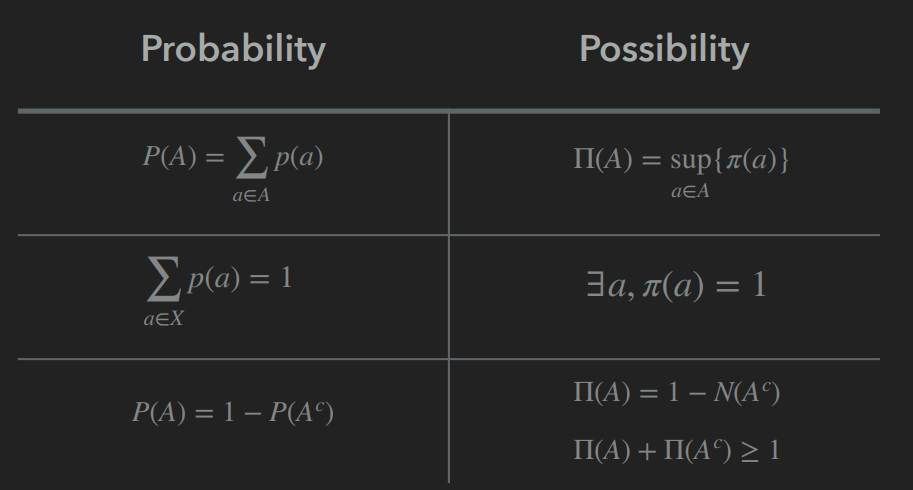
\includegraphics[width=0.5\textwidth]{img/sistemi_incerti/diff_prob_poss.png}
\end{figure}

Un caso particolare sono le funzioni booleane, funzione caratteristica di un insieme
ma che specificaun assegnamento di verità parziale. Quindi posso vedere un assegnamento 
parziale come un ortocoppia.

Posso vedere le belief function come un assegnamento di prob. agli insiemi, invece 
la probabilità è un assegnamento ad un evento.
\subsection{Belief function, Evidence theory and Dempster-Shafer}
Dalla capacità si deriva:
\begin{itemize}
    \item \textbf{probabilità}: capacità additiva
    \item \textbf{belieaf/plausibility function}
    \item \textbf{necessity/possibility}: capacità minitiva/massitiva
\end{itemize}

L'idea è di associare delle probabilità ad osservazioni incomplete e imprecise.
Il valore di verità deriva dall'insieme ma l'elemento esatto non lo si conosce.

\begin{definizione}[\textbf{Mass function}]
    Sia $X$ un insieme di esiti di esperimenti, sia $A\subseteq X$, possiamo associare
    ad un evento una \textbf{distribuzione di massa} $m:2^X\to [0,1]$ tale che:
    \begin{itemize}
        \item $m(\emptyset) = 0$
        \item $\sum_{A\subseteq X}m(A) = 1$
    \end{itemize}
\end{definizione}

Stiamo associando una distribuzione di probabilità agli insiemi

\begin{definizione}
    $A$ si chiama \textbf{focal set} se $m(A)>0$ 
\end{definizione}

\begin{nota}
    l'interpretazione della distribuzione ha un significato di un punto di vista 
    di tipo  epistemico ovvero si basa sulla nostra conoscenza soggettiva. Più precisamente $m(A)$ specifica che l'agente 
    conosce $x$ è in $A$. La massa può non essere monotona $A\subseteq B$ allora 
    $m(B)\le m(A) $ se l'agente è abbastanza sicuro che $x$ è in $A$. Se $m(X)=1$
    allora l'agente non sa niente. 
\end{nota}

Possiamo definire
\begin{definizione}[\textbf{Belief function}]
    La \textbf{belief function} $Bel:2^X\to [0,1]$ indica il totale della massa certa in $A$
    $$Bel(A) = \sum_{B\subseteq A} m(B)$$
\end{definizione}
\begin{definizione}[\textbf{Plausibility function}]
    La \textbf{plausibility function} $Pl:2^X\to [0,1]$ indica il totale della massa possibile in $A$
    $$Pl(A) = \sum_{B\cap A \ne \emptyset} m(B)$$
\end{definizione} 

Abbiamo che $Bel\le Pl$ e sono duali ovvero $Pl(A) = 1- Bel(A^c)$.

\begin{nota}
    Ricorda che $m(\emptyset) = 0$
\end{nota}

Le distribuzioni di massa rappresentano la conoscienza a priori e le possiamo 
unire effettuando \textbf{dempster's rule}
\begin{definizione}
    Date $m1,m2$ distribuzini di massa:
    \begin{itemize}
        \item $m_{1,2}(\emptyset) = 0$
        \item $m_{1,2} (A) = \frac{1}{1-K}\sum_{B\cap C =A}m_1(B)m_2(C)$
        dove $K =\sum_{B\cap C =A}m_1(B)m_2(C)$ è la misura di conflitto.
    \end{itemize}
\end{definizione}

Questa regola va bene solo quando le distribuzioni di massa impongono dei vincoli
sulla situazione, predilige i punti in comune.

Esistono altre regole di aggregazione:
\begin{itemize}
    \item \textbf{non normalizzata}: $m_{1,2}(A) =\sum_{B\cap C =A}m_1(B)m_2(C)$
    \item \textbf{unione}: $m_{1,2} (A)=\sum_{B\cup C =A}m_1(B)m_2(C)$
\end{itemize}

Generalmente:
\begin{itemize}
    \item sotto l'ipotesi di mondo chiuso meglio la normalizzata
    \item sotto l'ipotesi di mondo aperto meglio la non normalizzata.
\end{itemize}

Se la distribuzione di maassa è sul singolo elemento e non sugli insiemi si ottiene 
la probabilità. Otteniamo invece la misura di necessità se i set focali sono uno incluso nell'altro.
Dalle belief si possono ottenere l'approssimazione rough se i focal set sono una partizione.
Quindi catturo rappresentazioni rough basate su relazione di equivalenza.

Per ora abbiamo visto solo misure quantitative, passiamo definire delle \textbf{misure qualitative}, 
in cui si associa quindi un valore da un insieme ordinato (ordine totale).

Dato un universo $X$, definiamo $\mu:2^X\to L$ dove $L$ è un insieme con ordine 
totale in cui gli elementi esprimono credenza.

\section{Misure di incertezza}
La misura principale per misurare l'incertezza è l'entropia e ne esistono di diverse 
tipologie.

$X$ è un insieme di possibili alternative con associate delle probabilità 
e solo una alternativa è possibile. Come possiamo quantificare il fatto che $x$ 
occorre? 
L'idea è di definire una funzione:
\begin{itemize}
    \item \textbf{decrescente}: più è probabile che 
    occorre $x$ allora meno entropia ha
    \item \textbf{additiva}: se $p(x,y) = p(x)\cdot p(y)$ allora 
    $$u(p(x,y)) = u(p(x)) + u(p(y))$$
\end{itemize}

Esistono diverse tipologie di entropia:
\begin{itemize}
    \item \textbf{Shannon}:  
    $$u(p(x)) = K\log_b(p(x))$$
    dove $b = 2$ se si rappresenta in $b$ mentre $-1$ per la normalizazione.
    L'incertezza associata ad un insieme è 
    $$H(X) = - \sum_{x\in X}p(x)\log_2(p(x))$$
    Questo misura il contenuto informativo atteso di $X$.

    \item \textbf{Ellerman}: misura il contenuto informativo di una partizione $\pi$.
    L'entropia è alta tanto quanto l'abilità di distinguere tra due alternative.
    Per esempio quando abbiamo una classe che include tutti gli elementi allora non 
    si ha l'abilità di distinguerli e quindi abbiamo poca informazione. Al contrario 
    quando abbiamo una classe di equivalenza per ogni elemento allora abbiamo 
    massima informazione.

    Il calcolo si basa sui \textbf{dits} (distinction): coppie ordinate $(u_i,u_j)$
    di elementi in blocchi differneti:
    $$dit(\pi) = \{(u_i,u_j)| u_i,u_j \text{ classi che riesco a distinguere }\pi\}$$
    $$H(\pi) = \frac{|dit(\pi)|}{|U\times U|}$$
    utile quando dobbiamo creare delle orthopartition.
\end{itemize}

Possiamo introdurre delle misure di entropia più generalizzate:
\begin{itemize}
    \item \textbf{fuzzy entropy}: dato un fuzzy $f:X\to [0,1]$  
    $$H(f) = -\sum_{x\in X }\left[ f(x)\log_2f(x) + (1-f(x))\log_2(1-f(x))\right]$$
    Misura il grado di fuzzyness, quando $h(f) = 0$ quando è un insieme booleano,
    altrimenti massimo quando $\forall x, f(x) = \frac{1}{2}$. Dati due fuzzy $f_1,f_2$
    allora l'entropia misura anche la relazione di fuzzyness ovvero $f_1\le f_2 \iff H(f_1)\le H(f_2)$
    \item \textbf{conflitto di evidenza}: misura quanto sono in conflitto due distribuzioni 
    di massa $m_1,m_2$. Due distribuzioni sono in conflitto se $m_1(A)\ne 0, m_2(B)\ne 0$ 
    $A\cap B=\emptyset$ allora 
    $$con(m_1,m_2) = -\log_2(1-K)$$
    dove $K=\sum_{A\cap B=\emptyset}^{m_2(A)\cdot m_2(B)}$ e $A,B$ sono insiemi 
    focali. Dove $con$ è monotona crescente rispetto a $K$:
    \begin{itemize}
        \item $con(m_1,m_2) = 0$ sse $m_1,m_2$ non sono totalmente in conflitto ($K=0$)
        \item $con(m_1,m_2) = \infty$ sse $m_1,m_2$ sono totalmente in conflitto ($K=1$)
    \end{itemize}
    Possiamo calcolare il conflitto all'interno di una distribuzione di massa $m$. Per 
    fare ciò dobbiamo specificare una distribuzione fittizia
    $$m_A(B) = \begin{cases}
        1 & B=A\\
        0&altrimenti
    \end{cases}$$
    La quantità di conflitto di un focal set  con tutti gli altri focal set è 
    $$con(m,m_A) = -\log_2(1-\sum_{B\cap A=\emptyset}m(B))=-\log_2Pl(A)$$
    Possiamo calcolare la media su tutti gli insiemi focali:
    $$E[m] = \sum_{A\in F}m(A)conn(m,m_A) = -\sum_{A\in F}m(A)\log_2Pl(A) $$
    con $F$ focal sets.
    Se $m$ è una distribuzione di probabilità quindi assegna una distribuzione 
    ai singoli elementi allora $E[m]$ è l'entropia di shannon.
    Il conflitto è anche chiamato \textbf{dissonance}. Se i focal set sono tutti 
    $$A_1\subseteq A_2 \subseteq \dots \subseteq A_n$$
    Allora $E[m]= 0$, possibilità e necessità è senza conflitto.
    \item \textbf{confusione di evidenza}: dal conflitto possiamo ottenere la confusione 
    usando $Bel$:
    $$C[m]=-\sum_{A\in F}m(A)\log_2Bel(A)$$
    Se $C[m]=0$ sse $m(A)=1$ per un particolare $A$ e $m(B)=0$ tutti gli altri.
    $C[m]$ caratterizza:
    \begin{itemize}
        \item più la distribuzione è uniforme allora più siamo confusi
        \item se conconcentriamo su un insieme focale allora la confusione è $0$.
    \end{itemize}
    \item \textbf{Ellerman} sulle orthopartition: Sia $\mathcal{O}$ una orthopartizione 
    allora $\sqcap_\mathcal{O}$ è l'insieme di tutte le partizioni consistenti con $\mathcal{O}$.
    quindi $\pi \in \sqcap_\mathcal{O}$ possiamo calcolare $H(\pi)$ (con quella di Ellerman) e successivamente 
    calcolare l'entropia della orthopartition:
    \begin{itemize}
        \item lower entropy:
        $$h_\ast(\mathcal{O}) = \min\{H(\pi)|\pi \in \sqcap_\mathcal{O}\}$$
        \item upper entropy:
        $$h^\ast(\mathcal{O}) = \max\{H(\pi)|\pi \in \sqcap_\mathcal{O}\}$$
        \item mean entropy:
        $$\hat{h}(\mathcal{O}) = \frac{h_\ast(\mathcal{O}) + h^\ast(\mathcal{O})}{2}$$
        \item avg entropy:
        $$h_A(\mathcal{O})= \frac{1}{|\sqcap_\mathcal{O}|}\sum_{\pi \in \sqcap_\mathcal{O}}H(\pi)$$
    \end{itemize}
    \item \textbf{Shannon} sulle orthopartition: abbiamo bisogno di una distribuzione 
    $p=\left[p_1,\dots,p_n\right]$ che sia compatibile con l'orthopartizione.
    $$\mathcal{P}_\mathcal{O} = \{\left[p_1,\dots, p_n\right] | p_i\in \left[\frac{|P_i|}{|U|},\frac{|P_i\cup Bnd_i|}{|U|}\right], \sum_{i=1}^{n}p_i=1\}$$
    \begin{itemize}
        \item lower entropy:
        $$h_{S\ast}(\mathcal{O}) = \min\{H_S(\pi)|\pi \in \sqcap_\mathcal{O}\}$$
        \item upper entropy:
        $$h_S^\ast(\mathcal{O}) = \max\{H_S(\pi)|\pi \in \sqcap_\mathcal{O}\}$$
        \item mean entropy:
        $$\hat{h}(\mathcal{O}) = \frac{h_{S\ast}(\mathcal{O}) + h_S^\ast(\mathcal{O})}{2}$$
        \item avg entropy:
        $$h_{SA}(\mathcal{O})= \frac{1}{|\sqcap_\mathcal{O}|}\sum_{\pi \in \sqcap_\mathcal{O}}H_S(\pi)$$
    \end{itemize}
\end{itemize}


Per valutare il soft clustering si usano le ortopartizioni e si applica l'entropia.
L'entropia mi rappresenta le possibili coppie ordinate che possiamo distinguere.

Il problema è che non è efficiente perché si entra nel combinatorio
e quindi spesso si usano delle euristiche. Oppure possiamo usare l'entropia di 
Ellerman che sono polinomiali.

Nelle orthopartizioni spesso si calcola la misura di mutua informazione, ovvero 
l'informazione comune tra due orthopartizioni. 

$$m(\mathcal{O}_1,\mathcal{O}_2) = h(\mathcal{O}_1) + h(\mathcal{O}_2) - h(\mathcal{O}_1\land \mathcal{O}_2) $$
Dove $h$ è una qualsiasi entropia definita e $\mathcal{O}_1\land \mathcal{O}_2$ è 
l'intersezione.

$$\mathcal{O}_1\land \mathcal{O}_2=\{O_{i1}\sqcap_t O_{j2}|O_{i1}\in \mathcal{O}_1 \land O_{j2}\in\mathcal{O}_2\}$$

dove $O_{i1}\sqcap_t O_{j2} = (L_1\cap L_2, U_1\cup U_2)$
L'intersezione si calcola con l'intersezione dell'approssimazione dal basso e l'unione del boundary. Si usa 
questa perché coincide con l'intersezione tra partizioni delle due orthocopie. Menomale che Silvio c'è!

\section{Unione sistemi incerti e sistemi complessi}
sistemi tempo discreto e spazio discreto e pazio finito. L'idea è di capire incertezza 
e complessità in ml.

Nella vita reale in sistemi complessi possiamo osservare solo una parte del mondo 
e tutto il resto è incerto.

\begin{definizione}[\textbf{Sistema dinamico deterministico}]
    Un \textbf{sistema dinamico deterministico} è una coppia $(X,f)$ tale che 
    $f:X\to X$  che seleziona lo stato successivo
\end{definizione}

Quando i sistemi dinamici sono non deterministici allora questo introduce incertezza,
perché la transizione determina diversi stati raggiungibili ma non si conosce
quello preciso.

\begin{definizione}[\textbf{Sistema dinamico non deterministico}]
    Un \textbf{sistema dinamico non deterministico} è una coppia $(X,f)$
    $(X,f)$, $f:X\to 2^X$  che seleziona un insieme di stati possibili successivi.
\end{definizione}

questo coincide col dire che lo stato successivo può essere uno dei tanti successivi,
perché quando abbiamo un'osservazione parziale allora passiamo avere diversi possibili 
stati successivi.

Per ogni sistema deterministico possiamo associare un grafo che mostra il passaggio 
da uno stato all'altro attraverso transizioni, questo mostra se si ha determinismo 
o meno. (formalismo per rappresentare un qualsiasi sistema dinamico a tempo discreto 
e a stato discreto) Per quelli continui si discretizza.


Reaction system modellano i processi chimici. Si formalizzano mediante $3$ insiemi di sostanze:
\begin{itemize}
    \item reagenti
    \item inibitori
    \item prodotti
\end{itemize}
La stessa sostanza può essere prima un reagente, poi un inibitore e poi un prodotto.
Poi abbiamo l'insieme delle reazioni, sono le regole che si chiamano reazioni.
Formalmente si descrivono $(S,A)$ $S$ sostanze $A$ regole. Le regole sono triple 
$(R\subset S, I\subset S, P\subset S)$ dove se $R=S$ e $I=\emptyset$ allora $P=R$.

\begin{esempio}
    $S=\{H,O,H_2O\}$ allora una regola è $R=\{H,O\}$ $I = \{\}$ $P=\{H_2O\}$.
\end{esempio}

\begin{esempio}
    Sia $S=\{A,B,C\}$ le regole possono essere:
    \begin{itemize}
        \item $(\emptyset, ABC,BC)$
        \item $(B, C,AB)$
        \item $(A, C,AB)$
        \item $(C, AB,AC)$
        \item $(AB, \emptyset,ABC)$
    \end{itemize}
    Tutte le regole vengono applicate in parallelo e quindi il risultato è l'unione 
    dei risultati di tutte le regole applicabili
\end{esempio}

Possiamo rappresentare anche le reti di petri.

Vogliamo modellare l'incertezza con un unico linguaggio per tutti i sistemi dinamici.

Un primo modo per modellarli universalmente è attraverso il grafo ma essendo semplice 
perdo informazioni.
\begin{definizione}[\textbf{pattern}]
\end{definizione}
Un pattern rappresenta un pezzo di informazione rispetto allo stato del sistema.
(in questo stato è presente una sostanza)
\begin{definizione}[\textbf{Spazio di pattern}]
    Lo \textbf{spazio di pattern} è una tripla $(P,\le, \sim_m)$ dove:
    \begin{itemize}
        \item $P$ è l'insieme di pattern
        \item $(P,\le)$ è un poset
        \item $\sim_m$ è una relazione di equivallenza sugli insiemi minimali di $P$
    \end{itemize}
    Deve valere che presi $p_1,p_2\in P$ tale che $p_1\sqcup p_2$ esiste sse $\exists
    p_1'\le p_1, p_2'\le p_2$ tale che $p_1'\sim_mp_2\implies p_1' = p_2'$.
\end{definizione}
La relazione d'ordine esprime il concetto di generalità mentre la relazione di equivalenza 
è sui pattern minimali ovvero quello specifico.


\begin{definizione}[\textbf{Pattern dynamical system}]
    \textbf{Pattern dynamical system} è una quindtupla 
    $$(X, f, \mathcal{P},g, h)$$
    dove:
    \begin{itemize}
        \item $(X,f)$ è un sistema dinamico
        \item $\mathcal{P} = (P, \le, \sim_m)$ è un pattern spece
        \item $h:X\to M$ dove $M$ è l'insieme di elementi massimali, la funzione 
        deve essere un isomorfismo (gli elementi massimali di descrivono lo stato)
        \item $g:X\to 2^P$ dove $g(x)$ è l'ideale principale in $h(x)$ (sono tutti 
        gli elementi che stanno sotto $h(x)$, ovverlo tutti elementi $\le h(x)$)
    \end{itemize}
\end{definizione}

Aggiungo più informazioni al sistema dinamico astratto ($(X,f)$)

\begin{esempio}
    Nei sistemi reattivi l'informazione è quale sostanza appartiene e quale no.
    Quindi $P=S\cup \overline{S}$, $S$ sono le sostanze che sono presenti e $\overline{S}$
    le sostanze assenti. Un pattern $p=\{a,b,\overline{c}\}$ non è detto che ci 
    siano tutte le sostanze. La relazione $\le$ è la relazione di specificità. Se 
    $p_1\subseteq p_2$ allora $p_1\le p_2$, ex: $\{a,b\}\le \{a,b,\overline{c}\}$.
    
    La relazione di equivalenza $\sim_m$ associa simboli simili ex: $a\sim_m \overline{a}$
    (ovvero la contraddizione). 

    Esiste un pattern join solo quando esistono 2 elementi minimali che sono esattamente
    uguali.

    $h(x)$ mapperà gli stati nei pattern più specifici, $h(ab) = ab\overline{c}$

    $g(x)$ rappresenta per ogni stato quali informazioni sono vere, ex: $g(ab)=a,b, \overline{c}, a\overline{c}\dots$.
\end{esempio}

Il tipo di incertezza che avremo sui sistemi dinamici coincide con l'applicazione 
di un test che mi da delle informazioni parziali sullo stato attuale e quello che 
ci interessa è trovare le sottoinformazioni dello stato scoperto che ci viene descitto 
dal testo.

\begin{definizione}
    Sia $$APDS= (X,f, \mathcal{P}, g,h,T)$$ ddove $T$ è un insieme di test che ci dicono 
    se dei pattern sono veri oppure no in un certo pattern.
\end{definizione}
\begin{definizione}
    Quuindi $t:\mathcal{P} \to \{T,F\}$ che restituisce true o false se il pattern 
    è presente nello stato oppure no. Il test deve essere:
    \begin{itemize}
        \item monotona crescente: $p_1\le p_2 \implies t(p_1)\le t(p_2)$
        Questo mi dice che $x:t(x)= \sqcup_{p\in g(x)} t(p)$
    \end{itemize}
\end{definizione}

Questi test introducono delle delle approssimazioni perché possono ritornare valori 
uguali per stati differenti. Questo mi porta a modellare l'incertezza come Roughset

Quindi dato un insieme di test $T$, abbiamo uno stato $x$ allora $[x]_T$ è la 
classe di equivalenza $x$ su un insieme di test $T$. Quindi possimao definire 
la routhapproximation di uno stato $x$ è $r(x) =(l(x), u(x))$ tale che 0
$$l(x) = \bigcap_{y\in [x]_T} g(y)$$
$$u(x) = \bigcup_{y\in [x]_T} g(y)$$

PEr un qualsiasi test possiamo calcolare il supporto ovvero l'insieme per cui il 
test è vero.

Dai test si ottengono le classi di equivalenza degli stati, dalle quali si ottiene 
la rough approx delle classi di equivalenza e quindi si può avere del sistema dinamico 
rappresentato come rough approx. Quindi si collassano gli stati nelle classi di 
equivalenza e nella rappresentazione con rough abbiamo la fraccia tra rough solo 
se esiste un arco da un nodo di una classe ad un'altra. Con questa trasformazione 
rischiamo di perdere il determinismo.

Possiamo avere un'altra incertezza dipendente dall'osservazione dell'evoluzione 
di uno stato
\begin{definizione}
    Un osservazione $O$ è una collezioni di cammini massimale (aciclico) 
\end{definizione}
Ogni cammino massimale è un'osservazioene.

Se introduciamo delle opprossimazioni allroa le osservazioni possono cambiare 
le osservazioni a causa dei test che creano un'approssimazione.

Ora ci interessa sapere se i test permettono di riconoscere il comportamento del 
sistema oppure se un test non è infomrativo, per fare ciò si sfruttano i Reduct.

Si rappresenta il sistema dinamico con l'information table, in questo modo Vogliamo
trovare il reduct dei test.

Dato un insieme di test  $T$ allora $F\subseteq T$:
\begin{itemize}
    \item $F$ è un superreduct totale (un super insieme di un reduct) è un reduct 
    senza la minimalità se non mi cambia il grafico della dinamica
    \item $F$ è un superreduct parziale se nel caso due stati appartengono alla calsse 
    di equivalenza allora possono rimanere così, se due stati non sono nella stessa classe 
    allora si preservano le stesse classi.
    \item $F$ è un superreduct locale la dinamica non cambia limitatamente all'osservazione
\end{itemize} 
Trovare un sup-reduct totale allora è polinomiale 

In un reaction sistem è Np-Hard perché è polinomiale nella dimensione del grafo 

In generale il reduct minimale è Np-completo.


\section{MLOps}
Si ha l'algoritmo di apprendimento, diamo in input un insieme di dati e una topologia della rete allora in output 
otterremo il modello con i parametri. Successivamente col modello effettueremo le predizioni.


Possiamo avere 2 tipi di incertezza:
\begin{itemize}
    \item sui dati di training: si effettua un campionamento dei dati reali che può essere schematizzato attraverso un 
    generatore di dati $\mathcal{D}$, questo contiene incertezza sui dati come bias, errori sui dati, missing o imprecisione.
    \item sui dati di predizioni: si vuole comunicare l'incertezza, ovvero dal momento che abbiamo in input incertezza allora vogliamo 
    quantizzare questa incertezza, stima della probabilità che la predizione sia corretta. (uncertanty quantification)
\end{itemize}





\section*{Uncertanty quantification nella classificazione (supervisionato)}

Abbiamo uno spazio $X$ (feature space) rappresentazione degli oggetti che voglio studiare. e poi si ha $Y$ che è il target space. EX:
$X$ insieme di immagini mentre $Y$ sono le etichette associate. Se $Y$ è numerabile allora è classifivazione (binaria) altrimenti se è almento la 
cardinalità del continuo allora si parla di regressione.

$\mathcal{D}(X, Y)$ è il data generation mekanism, ovvero $\mathcal{D}(X, Y)$ è la probabilià di pescare la coppia $X,Y$ se $\forall x \exists !y\mathcal{D}(x,y)=1$
allora è un problema deterministico, altrimenti no (ex: riconoscere una malattia man on bastano i sintomi per riconoscerla). Si assume 
che non valga il determinsmo.

Si denota $\mathcal{D}(X)=\mathcal{D}(y=!|x) = E[y|x]$ perché siamo in una distribuzione di bernulli quindi il valore atteso è la probabilità 
di pescare la classe positiva. $\mathcal{D}(X)$ è l'incertezza aleatorica ed è un'incertezza che non può essere eliminata perché è una caratteristica
del meccanismo di generazione dei dati ed è quella che vogliamo quantificare. 

Il problema è che non conosciamo perché se lo conoscessimo allora possiamo definire il \textbf{classificatore}
perfetto quinid $h(x)=E[y|x]$. noi ci vogliamo avvicinare il più possibile e quindi definiremo una loss $l:H\to \mathbb{R}$.
La più semplice è la zero loss  $z(h)-1$ ovvero $1-accuracy$ il problema di usare l'accuracy è che non c'è un'inica soluzione giusta 
perché non è una funzione convessa. Generalmente si usano altre funzioni di loss come $L_2$ (squared-error).

Noi vogliamo trovare un modello tale che 
$$\arg\max_h E_x[(h(x)-E[y!x])^2]$$
Ma noi possiamo approssimarlo con 

$$\arg\max_h E_{x,y}[(h(x)-y)^2]$$
perché vediamo le etichette dal dataset, inoltre possiamo approssimare il valore atteso con la media campionaria
$$\arg\max_h \frac{1}{2}\sum_{(x,y)}[(h(x)-y)^2]$$

e questo è un upperbound dell'errore vero effettivo.

Se il nostro errore è $\alpha$ allora il modello è $\alpha$-valido, l'obiettivo è trovare $0$-valido che è impossibile perché non 
conosciamo la distribuzione marginale. 

Un modo per calcolare $\alpha$ è approssimarlo, perché non possiamo calcolare correttamente perché ci servono tutti i dati,
$\alpha = |E_x[h(x)]-E_{x,y}[y]|$ che è $\alpha$-mean marginally consistant che mi specifica il la predizione media sulle etichette medie.
Questo non mi dice che il mio classificatore è quello corretto ma se non è $0$-mean marginally consistant allora non lo è sicuramente.
Possiamo ottenere da un modello il suo $0$-mean marginally consistant  allora sia $\Delta = E_{x,y}[y]-E_x[h(x)]$ allora posso 
definire $h'(x) = h(x) +\Delta$ che è $0$-mean marginally consistant perché correggo le predizioni con il suo errore. 

Per calcolarl oeffitivamente userò le medie campionarie al posto dei valori attesi ma è sempre un'approssimazione con errore $\sqrt{\frac{\log(1/\delta)}{2n}}\ge \alpha$ ($\alpha$ reale col valore atteso).
dove $n$ è la dimensione del dataset ma $\delta$ è la confidenza.

Il problema è che sto guardando le singole istanze ma le medie delle istanze.
Un modo migliore è la calibrazione

Supponiamo che per un'istanza $x$ il modello predice $p=h(x)$ noi lo interpretiamo come probabilità ma non sempre questo è vero.

Se $P(y=1|h(x)=p)= p$ allora il modello è calibrato allora possiamo interpretare come probabilità se $P(y=1|h(x)=p)\ne p$ allora 
il modello è scalibrato e $p$ non coicide con la probabilità (maggior parte delle volte). In generale si sovrastima le probabilità della 
classe negativa e si sottostima le probabilità della classe negativa.

Il predittore di bayes è calibrato quindi tutti modelli scalibrati allora non è il predittore corretto.

Dobbiamo capire se è possibile calcolare se il modello è calibrato e nel caso correggere la calibrazione (è possibile). Per farlo facciamo 
l'assunzione che l'insieme di tutti gli score che mi può dare è finito $|V=\{h(x), x\in X\}|<\infty$ e questo non è troppo restrittivo perché
su pc tutto è finito.

Si introducono 2 metriche $ECE$ (expected calibration error) 
$$ECE = \sum_{v\in V}P(h(x)=v)|v-E[y|h(x)=v]|$$
$$K_2 = \sum_{v\in V}P(h(x)=v)(v-E[y|h(x)=v])^2$$
Anche per queste metriche non si possono calcolare perché dobbiamo conoscere la distribuzione generatrice.

Possiamo sempre correggere l'errore di calibrazione attraverso un algo iterativo di $T$ step dove ad ogni step 
riduco l'errore, ad ogni step calcolo 
$$v^\ast = \arg\max_{v\in V}P(h(x)=v)|v-E[y|h(x)=v]|$$ 
e un altro ciclo for tale che $h(x)=v^\ast $ allora $h(x)=E[y|h(x)=v^\ast]$. 
In sostanza istanza per istanza correggo le prredizioni col valore corretto. Al limite si correggono tutti i valori.
LA probabilità e il valore atteso le calocliamo sul dataset per ottenere un upperbound. Il problema è che 
la complessità è molto elevata, esiste una versione senza il for su $T$, alla fine assicura la correttezza 
ma la complessità è sempre elevata per la cardinalità del dataset. Nella pratica si usa la tecnica 
di platt scaling che sfrutta un modello di machine learning che risolve un problema di regressione 
dove le feature sono $h(x)$ e l'output è $y$. Si risolve con la logistic regression,
ma non ha una certezza teorica sul risultato ma è più efficiente.
In questo caso il modello dipende dalle istanze, il problema è che si deve eseguire 
su dati mai visti ovvero su un (Calibration set).

Tornando al problema iniziale i modelli $h:X\to [0,1]$  si ha il problema che non 
è associato alla probabilità. Per risolverlo si può usare l'approccio di 
restituire $h_\tau :X\to 2^Y$ ovvero restituendo un insieme contenente la classe 
corretta con una certa confidenza (simile all'intervallo di confidenza). Si parla 
quindi di conformal prediction. Tutto si basa su test statistici.

Si parte dal modello costruito $h:X\to [0,1]$, si definisce una \textbf{conformity score}
function 
$$S:X\times \mathbb{Z} \to \mathbb{R}$$
\begin{esempio}
    $S(x,h) = |h(x)-y|$
\end{esempio}
Più alto è il valore di $S$ allora maggiore è l'errore sul'istanza. Avremo 
quindi un calibration set separato dal training set per cui calcoliamo per ogni
coppia $(x_1,y_1)\dot(x_n,y_n)$ calcoliamo $S_i$.

Definiamo un nuovo modello 
$$h'_\tau(x)=\{y\in Y, S(x,h)\le \delta\}$$
con $\delta = \tau$-quantile su $C$. 

Quindi in $C$ eisteranno un totale di $(1-\tau)(n-1)$ istanze tale che $S(x,h)\le \delta$.

L'idea è di identificare un insieme di etichette tale che con probabilità maggiore
di $1-\tau$ l'etichetta vera appartiene all'insiem ovvero 
$$P_{x,y}(y\not \in h'_\tau(x))\le \tau + \mathcal{O}(\frac{1}{n})$$
più grande è $\tau$ allora più è inutile.



\section*{Uncertanty quantification nel clustering (non supervisionato)}
